%! suppress = Ellipsis
%! suppress = Quote
%! suppress = LineBreak
%! suppress = Makeatletter
%! suppress = TooLargeSection
%! suppress = MissingLabel
\documentclass[12pt]{article}

% Fields
\usepackage{geometry}
\geometry{top=25mm}
\geometry{bottom=35mm}
\geometry{left=20mm}
\geometry{right=20mm}
% ------------------------------------------------

% Graphics
\usepackage{color}
\usepackage{tabularx}
\usepackage{tikz}
% https://tikz.dev/tikz-graphs
\usetikzlibrary{positioning, shapes.geometric, arrows, automata, graphs}
\tikzset{
    expr/.style={ellipse, draw=gray!60, fill=gray!5, very thick, minimum size=7mm, yshift=0.7cm},
    hexpr/.style={ellipse, draw=gray!60, fill=blue!15, very thick, minimum size=7mm, yshift=0.7cm},
    stmt/.style={rectangle, draw=gray!60, fill=gray!5, very thick, minimum size=5mm, yshift=0.7cm},
    decl/.style={rectangle, draw=blue!60, fill=gray!5, very thick, minimum size=5mm, yshift=0.7cm},
    hdecl/.style={rectangle, draw=blue!60, fill=blue!15, very thick, minimum size=5mm, yshift=0.7cm},
    subtree/.style={shape border rotate=90, isosceles triangle, draw=gray!60, fill=gray!5, very thick, minimum size=5mm, yshift=0.0cm},
}
\usepackage{blkarray}
\usepackage{graphicx}
\usepackage{forest} % https://tex.stackexchange.com/questions/198405/how-to-change-the-color-of-subtrees-in-tikz-qtree
% ------------------------------------------------

% Math
\usepackage{amsmath, amsfonts}
\usepackage{amssymb}
\usepackage{proof}
\usepackage{mathrsfs}
% Crossed-out symbols
% https://tex.stackexchange.com/questions/75525/how-to-write-crossed-out-math-in-latex
\usepackage[makeroom]{cancel}
\usepackage{mathtools}
% ------------------------------------------------

% Additional font sizes
% https://www.overleaf.com/learn/latex/Questions/How_do_I_adjust_the_font_size%3F
\usepackage{moresize}
% Additional colors
% https://www.overleaf.com/learn/latex/Using_colours_in_LaTeX
\usepackage{xcolor}
% \texttimes
\usepackage{textcomp}
% ------------------------------------------------

% Language
\usepackage[utf8] {inputenc}
\usepackage[T2A] {fontenc}
\usepackage[english, russian] {babel}
\usepackage{indentfirst, verbatim}
\usetikzlibrary{cd, babel}
% ------------------------------------------------

% Fonts
\usepackage{stmaryrd}
\usepackage{cmbright}
\usepackage{wasysym}
% ------------------------------------------------

% Code
% https://tex.stackexchange.com/questions/99475/how-to-invoke-latex-with-the-shell-escape-flag-in-texstudio-former-texmakerx
% Colored, requires --shell-escape compiling option
\usepackage{minted}
\setminted{xleftmargin=\parindent, autogobble, escapeinside=??, linenos, numberblanklines=false}
\usepackage{listings}
% ------------------------------------------------

% Custom commands
\newcommand{\vocab}[1]{\textbf{#1}} % new word for vocabulary
\newcommand{\point}[1]{{\color{blue}\textit{#1}}} % point out something in text
\newcommand{\sembr}[1]{\llbracket{#1}\rrbracket} % semantic brackets
\newcommand{\positive}{$+$} % item: pros
\newcommand{\negative}{{\color{red} $-$}} % item: cons
\newcommand{\comb}[1]{\mathbf{#1}}
\newcommand{\step}{\rightsquigarrow}
\newcommand{\term}[1]{\mathbf{#1}}
\newcommand{\ap}{~}
\newcommand{\termdef}{\coloneqq}
\newcommand{\subst}[3]{\left[#2 \mapsto #3 \right] #1}
\newcommand{\eqbeta}{=_\beta}
\newcommand{\eqeta}{=_\eta}
\newcommand{\iso}{\cong}
\newtheorem{task}{Упражнение}
% ------------------------------------------------

% Head
\usepackage{hyperref}
\usepackage{fancyhdr}
% ------------------------------------------------

% Bibliography
\usepackage{csquotes}
% https://tex.stackexchange.com/questions/3802/how-to-get-doi-links-in-bibliography
\usepackage{natbib}
\bibliographystyle{unsrtnat}
%\bibliographystyle{apalike}
%\bibliography{bib}
%\usepackage[backend=bibtex]{biblatex}
%\addbibresource{bib.bib}
%\addbibresource{bib}
% ------------------------------------------------

% Line numbers
% https://tex.stackexchange.com/questions/16010/number-every-line-of-pages
\usepackage{lineno}
\linenumbers
% ------------------------------------------------

% Enumerations
% https://tex.stackexchange.com/questions/10684/vertical-space-in-lists
\usepackage{enumitem}
\setlist{noitemsep} % nosep
%\renewcommand{\labelitemi}{$\triangleright$}
%\renewcommand{\labelitemii}{$\triangleright$}
%\renewcommand{\labelitemiii}{$\triangleright$}
%\renewcommand{\labelitemiv}{$\triangleright$}
% ------------------------------------------------

% Formatting
\usepackage{multicol}
% https://tex.stackexchange.com/questions/282869/putting-two-figures-side-by-side
\usepackage{subcaption}
% https://tex.stackexchange.com/questions/109467/footnote-in-tabular-environment
\usepackage{footnote}
\makesavenoteenv{tabular}
% ------------------------------------------------



\begin{document}

    \begin{center}
    {\LARGE ФП 2.0}
        \footnote{Автор Андрей Стоян (\texttt{andrey.stoyan.csam@gmail.com}).}
        \\
        осень 2025
    \end{center}

    \tableofcontents

    \newpage

    \section*{Введение}

    Данный курс посвящен основам теории языков программирования.
    Многие сложные концепции могут быть поняты как частные случаи некоторых простых фундаментальных принципов, которые, как правило, считаются общеизвестным фольклором, не требующим дополнительных пояснений.
    Однако, сложность в том, что эти знания рассеяны по книгам, статьям и ``культовым'' блог-постам, и требуется довольно много времени и сил для восстановления целостной картины.

    Цель данного курса --- собрать в одном месте такие фольклорные знания и организовать их в некоторую систему.
    Курс будет явным образом опираться на классические работы, исследующие принципы построения языков, и помогать в их изучении.
    Просмотр упоминаемых статей является важной частью самостоятельной работы в рамках курса.

    Под функциональным программированием, вынесенным даже в заголовок курса, понимается трепетное отношение к понятию эффекта, которое в ФП, в отличие от других школ мысли, не считается аксиоматической данностью, но предметом для изучения, сознательного конструирования и аккуратного обращения.
    Этот подход оказывается очень продуктивным как для изучения языков, так и для построения могущественных языковых конструкций. % todo стиль программирования с эффектами
    Кроме того, функциональные языки сравнительно просты, в результате чего новые идеи и подходы, как правило, зарождаются в них и распространяются далее.

    В качестве основного языка курса выбран Haskell, так как он, с одной стороны, воплощает в себе многие концепции, часто доведенные до некоторого логического завершения, и достаточно могуществен для кодирования других.
    С другой стороны, всё ещё является прикладным промышленным языком программирования.

    В связи с широтой контекста, данный курс не всегда является глубоким.
    Так, детали реализации в GHC или теор-категорные основания вещей могут даваться в общем виде и без конкретики.
    В то же время, в плоскости языкового дизайна через оптику функционального программирования курс пытается быть максимально подробным.

    Таким образом, данный курс может быть полезен тем, кто интересуется дизайном языков и красивыми обобщениями программистских концепций, хочет улучшить свои навыки проектирования API, или планирует вести практическую деятельность на функциональных языках.

    Пререквизитом к прохождению курса является знание основ функционального программирования: алгебраических типов данных, паттерн-матчинга, свёрток, параметрического полиморфизма, классов типов, базовых монад.
    Дополнительно будет полезным умение читать типовые дроби, знакомство с полиморфным $\lambda$-исчислением и кодированием Чёрча.


    \clearpage


    \section{Воспоминания о ФП}

    В этом разделе мы вспомним основные концепции функционального программирования и языка Haskell.

\subsection{Термы и редукция} \label{subsec:terms-reduction}

В ФП программы представляют собой выражения.
Выполнение программ --- редукция таких выражений до более простых.
Выражения можно представлять как в виде линейной записи символов, так и в виде дерева, для понимания которого не требуется знания вспомогательных правил ассоциативности и проч.

Основная идея функционального программирования --- $\lambda$-абстракция.
Она позволяет взять произвольное выражение и заменить его фрагмент на формальный параметр.
Формальный параметр должен быть задекларирован выше по дереву с помощью специальной $\lambda$-вершины.
Вместо формального параметра можно в дальнейшем подставлять различные конкретные параметры, то есть использовать одно выражение для различных целей.

\begin{figure}[h]
    \centering
    \begin{tikzpicture}
        \node [expr] (div) {$\div$};
        \node [expr] (x) [below left=of div] {$x$};
        \node [expr] (plus) [below right = of div] {$+$};
        \node [expr] (two) [below right = of plus] {$2$};
        \node [hexpr] (mult) [below left = of plus] {$\times$};
        \node [hexpr] (ten) [below left = of mult] {$10$};
        \node [hexpr] (four) [below right = of mult] {$4$};
        \draw[->] (plus) -- (div);
        \draw[->] (x) -- (div);
        \draw[->] (mult) -- (plus);
        \draw[->] (ten) -- (mult);
        \draw[->] (four) -- (mult);
        \draw[->] (two) -- (plus);
    \end{tikzpicture}
    \begin{tikzpicture}
        \node [hdecl] (f) {$f$};
        \node [hexpr] (lam) [below=of f] {$\lambda$};
        \node [hdecl] (y) [below right =of lam] {$y$};
        \node [expr] (div) [below=of lam] {$\div$};
        \node [expr] (x) [below left=of div] {$x$};
        \node [expr] (plus) [below right = of div] {$+$};
        \node [hexpr] (param) [below left=of plus] {$y$};
        \node [expr] (two) [below right = of plus] {$2$};
        \draw[->] (lam) -- (f);
        \draw[->] (div) -- (lam);
        \draw[->] (plus) -- (div);
        \draw[->] (x) -- (div);
        \draw[->] (two) -- (plus);
        \draw[->] (param) -- (plus);
        \draw[->] (y) -- (lam);
    \end{tikzpicture}
    \begin{tikzpicture}
        \node [hexpr] (app) {$@$};
        \node [hexpr] (f) [below left =of app] {$f$};
        \node [expr] (mult) [below right= of app] {$\times$};
        \node [expr] (ten) [below left= of mult] {$10$};
        \node [expr] (four) [below right= of mult] {$4$};
        \draw[->] (mult) -- (app);
        \draw[->] (f) -- (app);
        \draw[->] (ten) -- (mult);
        \draw[->] (four) -- (mult);
    \end{tikzpicture}
\end{figure}

Простейший функциональный язык --- $\lambda$-исчисление.
Выражения в нём называются $\lambda$-термами.
Термы можно сконструировать тремя способами:
\begin{description}
    \item[Переменные] $x \in \Lambda$, если $x \in V$ \hspace{2em}
    \begin{tikzpicture}
        \node [expr] (x) {x};
    \end{tikzpicture}
    \item[Абстракция] $(\lambda x\ldotp M) \in \Lambda$, если $x \in V, M \in \Lambda$ \hspace{2em}
    \begin{tikzpicture}
        \node [expr] (lam) {$\lambda$};
        \node [decl] (x) [below right = of lam] {$x$};
        \node [subtree] (m) [below = of lam] {$M$};
        \draw[->] (m.north) -- (lam);
        \draw[->] (x) -- (lam);
    \end{tikzpicture}
    \item[Аппликация] $(M~N) \in \Lambda$, если $M \in \Lambda, N \in \Lambda$ \hspace{2em}
    \begin{tikzpicture}
        \node [expr] (dog) {$@$};
        \node [subtree] (m) [below left= of lam] {$M$};
        \node [subtree] (n) [below right= of lam] {$N$};
        \draw[->] (m.north) -- (lam);
        \draw[->] (n.north) -- (lam);
    \end{tikzpicture}
\end{description}

Редукция определяется следующим правилом переписывания: ищется применение $\lambda$-функции к аргументу и в её тело осуществляется подстановка аргумента во все свободные вхождения переменной, связанной лямбдой.

\begin{figure}[h]
    \centering
    \begin{tikzpicture}
        \node [expr] (top) {$\cdots$};
        \node [hexpr] (ap) [below = of top] {$@$};
        \node [hexpr] (lam) [below left = of ap] {$\lambda$};
        \node [decl] (x) [below right = of lam] {$x$};
        \node [subtree] (l) [below = of lam] {$M$};
        \node [subtree] (r) [below right = of ap] {$N$};
        \draw[->] (ap) -- (top);
        \draw[->] (lam) -- (ap);
        \draw[->] (l) -- (lam);
        \draw[->] (r.north) -- (ap);
        \draw[->] (x) -- (lam);
    \end{tikzpicture}
    \begin{tikzpicture}
        \node [expr] (top) {$\cdots$};
        \node [subtree] (bot) [below = of top] {$\subst{M}{x}{N}$};
        \draw[->] (bot) -- (top);
    \end{tikzpicture}
\end{figure}

\subsection{Типы}

Программное обеспечение --- это сложно.
Поэтому постоянно и неизбежно в программах возникают ошибки.
Их можно искать, в том числе, статически, то есть без запуска программы.
Одним из видов статического анализа является анализ типов.

Как известно, выражение можно представить в виде дерева.
Для примера рассмотрим $(\lambda y\ldotp x \div (y + 2)) \ap 3$:
\\
\begin{figure}[h]
    \centering
    \begin{tikzpicture}
        \node [expr] (ap) {$@$};
        \node [expr] (three) [below right = of ap]{$3$};
        \node [hexpr] (lam) [below left =of ap] {$\lambda$};
        \node [hdecl] (y) [below right =of lam] {$y$};
        \node [expr] (div) [below=of lam] {$\div$};
        \node [expr] (x) [below left=of div] {$x$};
        \node [expr] (plus) [below right = of div] {$+$};
        \node [hexpr] (param) [below left=of plus] {$y$};
        \node [expr] (two) [below right = of plus] {$2$};
        \draw[->] (three) -- (ap);
        \draw[->] (lam) -- (ap);
        \draw[->] (div) -- (lam);
        \draw[->] (plus) -- (div);
        \draw[->] (x) -- (div);
        \draw[->] (two) -- (plus);
        \draw[->] (param) -- (plus);
        \draw[->] (y) -- (lam);
    \end{tikzpicture}
\end{figure}

Идея анализа типов состоит в том, что мы каждой вершине дерева программы пытаемся присвоить некоторую синтаксическую метку по определённым правилам.
Если каждой вершине метку присвоить можно, то мы считаем, что программа проходит проверку типов, и она ``хорошая''.

Пример выше проходит проверку типов в некоторой разумной системе типов:
\begin{figure}[h]
    \centering
    \begin{tikzpicture}
        \node [expr] (ap) {$@ : int$};
        \node [expr] (three) [below right = of ap]{$3 : int$};
        \node [hexpr] (lam) [below left=of ap] {$\lambda : int \to int$};
        \node [decl] (y) [below right = of lam] {$y {\color{red}~: int}$};
        \node [expr] (div) [below=of lam] {$\div : int$};
        \node [expr] (x) [below left=of div] {$x : int$};
        \node [expr] (plus) [below right = of div] {$+ : int$};
        \node [hexpr] (param) [below left=of plus] {$y : int$};
        \node [expr] (two) [below right = of plus] {$2 : int$};
        \draw[->] (lam) -- (ap);
        \draw[->] (three) -- (ap);
        \draw[->] (div) -- (lam);
        \draw[->] (plus) -- (div);
        \draw[->] (x) -- (div);
        \draw[->] (two) -- (plus);
        \draw[->] (param) -- (plus);
        \draw[->] (y) -- (lam);
    \end{tikzpicture}
\end{figure}

Система типов определяет синтаксис типовых меток и правила, по которым их можно приписывать.
Синтаксис обычно описывается в классических нотациях а ля BNF, а правила в виде типовых дробей.
Например, так выглядят дроби для просто-типизированного $\lambda$-исчисления:
\[
    \begin{array}{l c r}
        \infer[ctx]{\Gamma \vdash x: \sigma}{(x: \sigma) \in \Gamma}
        &
        \infer[elim\to]{\Gamma \vdash M\;N : \tau}{\Gamma \vdash M : \sigma \to \tau & \Gamma \vdash N : \sigma}
        &
        \infer[intro\to]{\Gamma \vdash \lambda x^{\color{red} \sigma}\ldotp M : \sigma \to \tau}{\{x : \sigma\} \cup \Gamma \vdash M : \tau}
    \end{array}
\]

Типовые метки имеют чисто-синтаксическую природу, однако их можно проинтерпретировать.
Самая популярная интерпретация~--- воспринимать типовую метку как множество.
Так, метке $int \to int$ можно поставить в соответствие множество функций между множествами ограниченных целых чисел.

\subsection{Функции в Haskell}

В своей основе Haskell представляет собой расширенное типизированное $\lambda$-исчисление, дополненное примитивными типами, возможностью декларировать новые имена, структурами данных и классами типов.

Примеры $\lambda$-абстракций в REPL окружении GHCi:

\begin{minted}{haskell}
    ghci> (\x -> x + 1) 4
    5
\end{minted}

Можно узнать тип функции в интерпретаторе (в реальности числа полиморфные, но об этом далее):
\begin{minted}{haskell}
    ghci> :t \x -> x + 1
    \x -> x + 1 :: Int -> Int
\end{minted}

Функциям можно давать имена.
Именам можно приписывать типы, это рекомендуется делать явно для деклараций на верхнем уровне файлов исходного кода.
\begin{minted}{haskell}
    f :: Int -> Int
    f x = x + 1
\end{minted}

Если имя типа начинается с маленькой буквы, то это не конкретный заранее заданный тип, а типовая переменная, способная принимать различные значения в зависимости от контекста.
Такая возможность называется \point{параметрическим полиморфизмом}.
Так, функция, которая просто возвращает свой аргумент, никак не ограничивает тип аргумента.
Но в то же время тип результата должен совпадать с типом аргумента.
\begin{minted}{haskell}
    id :: a -> a
    id x = x

    ghci> :t id 5
    id 5 :: Int
\end{minted}

Функции могут принимать другие функции в качестве аргументов.
Имя функции может состоять из специальных символов, тогда она считается оператором и может применяться к своим операндам в инфиксном стиле:
\begin{minted}{haskell}
    ($) :: (a -> b) -> a -> b
    f $ x = f x
\end{minted}

Пример рекурсивной функции, использующей охранные выражения для отличения базового случая рекурсии:
\begin{minted}{haskell}
    factorial :: Int -> Int
    factorial n
      | n < 1 = 1
      | otherwise = n * factorial (n - 1)
\end{minted}

\begin{task}
    Что выведет запрос \mintinline{haskell}|ghci> :t uncurry (flip const)|?
\end{task}

\begin{task}
    Что выведет запрос \mintinline{haskell}|ghci> :t first . first| при
    \begin{minted}{haskell}
        first :: (a -> a') -> (a, b) -> (a', b)
    \end{minted}
\end{task}

\begin{task}
    Реализуйте факториал с помощью техники аккумулирующего параметра.
\end{task}

\subsection{Данные в Haskell}

В Haskell есть встроенная возможность объявлять свои типы данных, а так же создавать их экземпляры.

Зададим тип данных, описывающий животных:
\begin{minted}{haskell}
    data Animal
      = Cat String Int
      | Dog String
\end{minted}

Мы задали тип данных \texttt{Animal} и два способа создать значения этого типа: для кошек и собак.
\texttt{Cat} и \texttt{Dog}~--- это \point{конструкторы данных}.
Они представляют собой функции, реализация которых находится на стороне языка.
Они выделяют память под экземпляры данного типа и возвращают их.
Кошек мы описываем именем и оставшимся количеством жизней, а собак~--- только именем.
\begin{minted}{haskell}
    Cat :: String -> Int -> Animal
    Dog :: String -> Animal
\end{minted}

Чтобы воспользоваться информацией, сохранённой в структуре данных, требуется деконструировать её с помощью паттерн-матчинга.
Мы сопоставляем значение типа с образцом.
Если образец похож на то, как было сконструировано значение, то он выбирается среди других образцов и переменные, задекларированные в нём, начинают ссылаться на соответствующее содержимое структуры данных:
\begin{minted}{haskell}
    show :: Animal -> String
    show animal = case animal of
      Cat name nLifes -> "This is cat " ++ name ++ show nLifes
      Dog name -> "This is dog " ++ name
\end{minted}

В Haskell есть специальный синтаксис для объявления полей с именованными метками.
\begin{minted}{haskell}
    data Penguin = Penguin { getName :: String, getAge :: Int }
    penguin = Penguin { getName = "Andrey", getAge = 500 }
\end{minted}
Haskell генерирует функции-аксессоры для доступа к полям объекта:
\begin{minted}{haskell}
    ghci> :t getName :: Penguin -> String
\end{minted}

Часто функции в программировании частичные --- при некоторых значениях аргументов они могут вернуть результат, а при некоторых~--- нет.
Давайте моделировать это с помощью специального типа данных.
Если есть целочисленный результат, будем возвращать его.
Если нет, будем возвращать специальное значение этого типа~--- \texttt{Nothing}.
\begin{minted}{haskell}
    data MaybeD = NothingD | JustD Double
    sqrt :: Double -> MaybeD
    sqrt x = if x < 0 then NothingD else JustD (calcSqrt x)
\end{minted}

Можно заметить, что так нам придётся объявлять по типу \texttt{MaybeT} для каждого типа \texttt{T}.
Поэтому Haskell позволяет абстрагироваться в типе, аналогично тому как можно абстрагироваться по значениям в терме.
\begin{minted}{haskell}
    data Maybe a = Nothing | Just a
    sqrt :: Double -> Maybe Double
    sqrt x = if x < 0 then Nothing else Just (calcSqrt x)
\end{minted}

Заметьте, что сейчас \texttt{Maybe} --- это не совсем тип, так как теперь нужно передать типовой параметр, чтобы получить конкретный тип.
\texttt{Maybe} называют \point{типовым конструктором}.
Однако нам не всегда будет принципиально и мы для краткости будем типовые конструкторы называть типами.

Вместе с абстракцией на уровне типов появилась и аппликация типа к типу.
А что если дать меньше параметров типовому конструктору, чем ожидается?
А что если больше?
Контроль за корректностью типовых аппликаций обеспечивает система кайндов.
Это простейшие ``типы для типов'', то есть синтаксические метки, контролирующие корректность построенных типов.
Так, обычные типы имеют метку (кайнд) \texttt{*}.
Типовые конструкторы имеют стрелочные кайнды.
Например, \texttt{Maybe :: * -> *}.
Аппликация типового конструктора к типу подходящего кайнда убирает одну стрелку:
\begin{minted}{haskell}
    ghci> :k Int
    Int :: *
    ghci> :k Maybe
    Maybe :: * -> *
    ghci> :k Maybe Int
    Maybe Int :: *
\end{minted}

Кроме совершенно новых типов данных в Haskell можно объявлять типовые синонимы.
Это имена, которые можно использовать вместо других типов, если, например, запись оригинального типа слишком длинная для повсеместного написания.
\begin{minted}{haskell}
    type T a = VeryLongType Int (a -> AnotherLongType a)
\end{minted}

Если тип данных содержит только один конструктор и только одно поле, то отсутствует необходимость в аллокации новой памяти, содержащей тег конструктора и набор ссылок на поля.
В таком случае, в качестве значения такого типа можно всегда просто использовать значение оборачиваемого типа, оставляя новый тип присутствовать исключительно во время компиляции, снижая нагрузку на время исполнения.
Для объявления таких типов-обёрток нужно воспользоваться ключевым словом \texttt{newtype} вместо \texttt{data}:
\begin{minted}{haskell}
    newtype CourseId = CourseId Int64
    newtype ModuleId = ModuleId Int64
\end{minted}

\begin{task}
    Определите кайнд конструктора типа
    \begin{minted}{haskell}
        data Free f a = Pure a | Free (f (Free f a))
    \end{minted}
\end{task}

\subsection{Классы типов в Haskell}

Рассмотренные ранее полиморфные функции ничего не могли делать со своими аргументами, кроме как возвращать их в качестве результата или передавать в другие полиморфные функции.
Чтобы уметь делать что-то ещё, нужна какая-то дополнительная информация про тип, потому что иначе нет никакой гарантии, что над объектом данного типа можно делать все необходимые операции.
Так, функция \texttt{suc n = n + 1} не будет работать для строчек, потому что для них, очевидно, не определена операция сложения.
Поэтому некорректно будет приписать полиморфный тип \texttt{suc :: a -> a}.

В Haskell есть механизм ограничения полиморфности функций~--- \texttt{классы типов}.
Мы можем явно задать, что функция требует не произвольный тип на вход, а произвольный тип, для которого определены обязательно нужные нам операции.
Так, для типа \texttt{suc} достаточно ограничить тип условием наличия плюса для него: \texttt{suc :: Num a => a -> a}.
Теперь типовая переменная \texttt{a} может быть специализирована только на типы, на которых определена операция сложения.

Пример объявления класса типов \texttt{Eq}:
\begin{minted}{haskell}
    class Eq a where
      (==) :: a -> a -> Bool
\end{minted}

Для каждого типа можно объявить свою собственную реализацию \texttt{Eq}.
Возможность использования такой индивидуальной реализации для каждого типа называется ad-hoc полиморфизмом.
\begin{minted}{haskell}
    instance Eq CourseId where
      CourseId x == CourseID y = x == y

    instance Eq a => Eq [a] where
      [] == [] = True
      x:xs == y:ys = x == y && xs == ys
\end{minted}

\begin{task}
    Реализуйте инстанс полугруппы для функций.
\end{task}

\begin{task}
    Реализуйте проверку равенства функций.
\end{task}

\subsection{Монады в Haskell}

Класс типов \texttt{Functor} объявляется для конструкторов типов и позволяет заменить в некотором контейнере все элементы одного типа на все элементы другого, оставляя структуру контейнера неизменной.

\begin{minted}{haskell}
    class Functor (f :: * -> *) where
      fmap :: (a -> b) -> f a -> f b

    instance Functor [] where
      fmap :: (a -> b) -> [a] -> [b]
      fmap _ [] = []
      fmap f (x:xs) = f x : fmap f xs
\end{minted}

В Haskell любая функция просто вычисляет результат некоторого типа.
Однако в программирования часто требуются функции, которые не только вычисляют результат, но и делают что-то ещё.
Например, изменяют какое-то состояние или пишут в консоль.
Иными словами, производят побочные эффекты.
В любом случае в Haskell мы можем только вернуть из функции только результат, поэтому такие побочные эффекты мы кодируем в качестве дополнительной структуры, оборачивающей чистый результат.
Т.е. если функция без побочных эффектов возвращала какой-то тип \texttt{a}, то после добавления побочных эффектов в её реализацию она будет возвращать некоторый тип \point{вычислений} \texttt{f a}.

\begin{itemize}
    \item Если функция кидает ошибку, то \texttt{f = Maybe}.
    \item Если функция читает глобальное состояние, то \texttt{f = e -> \_}.
    \item Если функция читает глобальное состояние и обновляет его, то \texttt{f = s -> (s, \_)}.
\end{itemize}

Стандартная библиотека Haskell предоставляет несколько классов типов для работы со значениями вида \texttt{f a}.
Они позволяют абстрагироваться от структуры \texttt{f} и работать со значениями \texttt{a} внутри, как будто нет никакой дополнительной структуры.

Первый такой класс типов позволяет писать выражения над вычислениями \texttt{f a}.
\begin{minted}{haskell}
    class Functor f => Applicative (f :: * -> *) where
      pure :: a -> f a
      liftA2 :: (a -> b -> c) -> f a -> f b -> f c

    instance Applicative Maybe where
      pure :: a -> Maybe a
      pure = Just

      liftA2 :: (a -> b -> c) -> Maybe a -> Maybe b -> Maybe c
      liftA2 _ Nothing _ = Nothing
      liftA2 _ _ Nothing = Nothing
      liftA2 f (Just x) (Just y) = Just (f x y)
\end{minted}

Второй класс типов позволяет делать последовательную композицию вычислений в императивном стиле:
\begin{minted}{haskell}
    class Applicative m => Monad (m :: * -> *) where
      (>>=) :: m a -> (a -> m b) -> m b

    newtype State s a = State { runState :: s -> (s, a) }

    instance Monad (State s) where
      (>>=) :: State s a -> (a -> State s b) -> State s b
      m >>= k = State \s ->
        let (s', x) = runState m s in
        runState (k x) s'
\end{minted}

Теперь если мы определим базовые операции работы с состоянием, мы сможем писать код в императивном стиле.
\begin{minted}{haskell}
    get :: State s s
    get = State \s -> (s, s)

    put :: s -> State s ()
    put newS = State \oldS -> (newS, ())

    example :: State Int Int
    example =
      get >>= \x ->
      put 42 >>= \() ->
      get >>= \y ->
      pure (x + y)

    ghci> runState example 1
    43
\end{minted}

Для таких монадических цепочек существует специальный синтаксический сахар:
\begin{minted}{haskell}
    example :: State Int Int
    example = do
      x <- get
      put 42
      y <- get
      pure (x + y)
\end{minted}

\begin{task}
    Реализуйте \mintinline{haskell}|liftA3| через \mintinline{haskell}|liftA2|.
\end{task}

\begin{task}
    Реализуйте \mintinline{haskell}|>>=| через \mintinline{haskell}|join| и наоборот.
\end{task}

\begin{task}
    Два числа с консоли, поделите одно на другое нацело и распечатайте результат, если остаток не нулевой, распечатайте его тоже.
\end{task}


    \clearpage


    \section{Общие знания о типах}

    В этой главе собраны некоторые общие знания о типах.

Разделы~\ref{subsec:isomorphism}, ~\ref{subsec:type-algebra}, ~\ref{subsec:variance} в основном следуют~\cite[глава 1]{maguire-types}.
С категорным взглядом на происходящее можно ознакомиться в~\cite{hinze2010reason}.

\subsection{Изоморфизм} \label{subsec:isomorphism}

Пусть нам нужно спроектировать функцию.
Мы начинаем с записи типа, как первой аппроксимации нужной семантики.
Но как выбрать тип?
Для начала поймём, когда два типа взаимозаменимы, для этого рассмотрим понятия изоморфизма.

Два типа \texttt{A} и \texttt{B} называются \vocab{изоморфными} (обозначают \texttt{A $\iso$ B}) тогда и только тогда, когда существует такая пара функций \texttt{to :: A -> B} и \texttt{from :: B -> A}, что\footnote{Под равенством термов можно понимать разное, например, $\alpha\beta\gamma$-эквивалентность. Мы будем пользоваться \vocab{экстенсиональным равенством}~--- две функции равны, когда равны их результаты на всех входах.} % todo link more
\begin{minted}{c}
    to . from = id
    from . to = id
\end{minted}

Иначе говоря, элементам одного типа можно поставить в соответствие элементы другого, и наоборот.
Легко понять, что со смысловой точки зрения не принципиально, какой из изоморфных типов использовать, если в любой момент можно получить соответствующий элемент другого типа, а потом вернуться в изначальный тип.
Такие два типа заключают в себе одинаковое ``количество информации''.
Например, типы \mintinline{haskell}|Bool| и \mintinline{haskell}|Maybe ()| в этом смысле совершенно взаимозаменимы.
Покажем это, предъявив пару взаимообратных функций\footnote{Нужно не забыть показать взаимообратность функций, но это делается тривиально перебором входов (может быть с помощью индукции) и редукцией.}:
\begin{minted}{haskell}
    to :: Bool -> Maybe ()
    to b = if b then Just () else Nothing

    from :: Maybe () -> Bool
    from m = case m of Nothing -> False; Just () -> True
\end{minted}

Несмотря на смысловую взаимозаменимость, для кодирования информации о том, передал ли пользователь программе определённый флаг, мы, скорее всего, воспользуемся типом \mintinline{haskell}|Bool| ввиду нефункциональных соображений о читабельности кода.
Аналогично можно рассматривать соображения эффективности.

\subsection{Кардинальность: суммы, произведения, экспоненты} \label{subsec:cardinality}

Типы можно воспринимать как синтаксис для записи множеств, а населяющие их термы~--- как синтаксические записи элементов этих множеств.
Так терм \mintinline{haskell}|(True, False)|~--- запись элемента множества пар, записываемого в синтаксисе типов как \mintinline{haskell}|(Bool, Bool)| (вместо математического $\mathbb{B}\times\mathbb{B}$).
Или же терм \mintinline{haskell}|\x -> x + 1| является записью функции прибавляющей единицу из множества функций над целыми числами, записываемого как \mintinline{haskell}|Integer -> Integer| (вместо математического $\mathbb{Z}\to\mathbb{Z}$).

Заметим, что два типа изоморфны, если соответствующие им множества имеют одинаковое количество элементов.
Более того, таких изоморфизмов $n!$ в случае конечности множеств.
Научимся определять количество таких элементов.
С помощью $|\cdot|$ будем записывать \vocab{кардинальность} типа~--- количество элементов в соответствующем множестве.

Рассмотрим следующие типы:
\begin{minted}{haskell}
    data Void
    data Unit = Unit -- Вместо Unit в Haskell пишут ().
    data Bool = False | True
\end{minted}

Количество элементов в этих типах очевидно:
\begin{itemize}
    \item $|Void| = 0$ --- тип не населён.
    \item $|Unit| = 1$ --- один одноимённый обитатель.
    \item $|Bool| = 2$ --- очевидно, два терма.
\end{itemize}

Идея алгебраических типов данных в том, что сложные типы можно строить из простых с помощью операции $+$ (``или'') и операции $\times$ (``и'')\footnote{\url{https://stanford-cs242.github.io/f18/lectures/02-2-algebraic-data-types.html}}.
Рассмотрим следующие декларации:
\begin{minted}{haskell}
    data Example = FirstAlternative Bool | AnotherOne Unit Bool Bool
    data Either a b = Left a | Right b
    data Pair a b = Pair a b
\end{minted}

Посчитаем количество обитателей различных типов:
\begin{itemize}
    \item $|Example| = |Bool| + |Unit| \times |Bool| \times |Bool| = 2 + 1 \times 2 \times 2 = 6$ --- вы можете убедиться в справедливости заключения перебрав все термы типа \mintinline{haskell}|Example| вручную.
    \item $|Either \ap Unit\ap (Eigher \ap Bool\ap Bool)| = |Unit| + (|Bool| + |Bool|) = 5$.
    \item $|Pair\ap (Either\ap Bool\ap Unit)\ap (Pair\ap Unit\ap Void)| = (|Bool| + |Unit|) \times (|Unit| \times |Void|) = 0$ ~--- тип \mintinline{haskell}|Void| не населён, как и кортеж, его включающий.
\end{itemize}

Функциональную стрелку называют экспоненциальным типом.
Действительно, количество обитателей \mintinline{haskell}|A -> B| вычисляется как \[|A \to B| = |B|^{|A|}\]















\subsection{Алгебраическое представление типа} \label{subsec:type-algebra}





% todo algebraic data types are relations between data https://stanford-cs242.github.io/f18/lectures/02-2-algebraic-data-types.html
% todo https://codewords.recurse.com/issues/three/algebra-and-calculus-of-algebraic-data-types

\begin{figure}[h!]
    \centering
    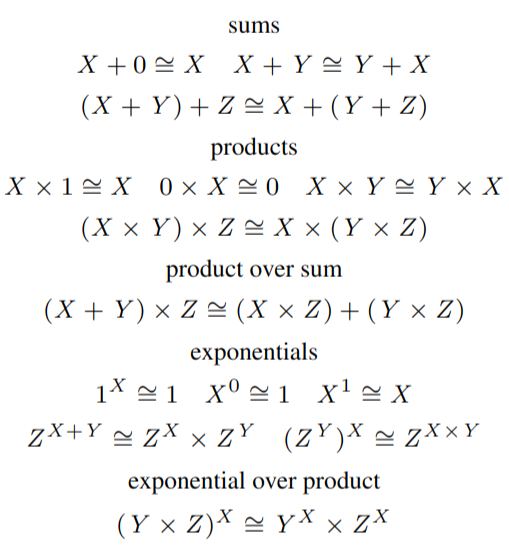
\includegraphics[width=0.4\textwidth]{figs/school-alg}
    \caption{Законы школьной алгебры ностальгии ради~\cite{hinze2010reason}.}
    \label{fig:school-alg}
\end{figure}

% todo isomorphismы и кардинальности
% todo reason isomorphically
% todo connection with cardinalities



% todo каноническое представление типа

TODO % todo

\subsection{Полярности и вариантность} \label{subsec:variance}

В этом параграфе мы будем рассматривать тему с точки зрения программирования~\cite[глава 3]{maguire-types}, не отдавая должного теории категорий.
Восполнить пробел можно с помощью замечательной статьи, написанной в жанре пьесы~\cite{hinze2012functional}.

\vocab{Ковариантный функтор} --- пара из типового конструктора \texttt{F} и операции на функциях \texttt{fmap :: (a -> b) -> (F a -> F b)}.
Плюс законы о том, что \texttt{fmap} уважает \texttt{id} и композицию.

\begin{minted}{haskell}
    class Functor f where
      fmap :: (a -> b) -> (f a -> f b)
\end{minted}

\begin{figure}[H]
    \centering
    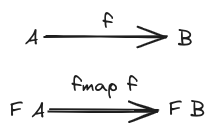
\includegraphics[width=0.3\textwidth]{figs/functor}
\end{figure}

\vocab{Контравариантный функтор} --- пара из типового конструктора и операции на функциях, разворачивающей стрелку.
Плюс соответствующие законы.

\begin{minted}{haskell}
    class Contravariant f where
      contramap :: (a -> b) -> (f b -> f a)
\end{minted}

\begin{figure}[H]
    \centering
    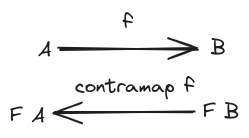
\includegraphics[width=0.3\textwidth]{figs/contra-functor}
\end{figure}

Типовой конструктор можно объявить ковариантным или контравариантным функтором (или никаким из них) относительно типового параметра в зависимости от вида декларации соответствующих конструкторов данных.
А именно, от \vocab{полярности}\footnote{\url{https://existentialtype.wordpress.com/2012/08/25/polarity-in-type-theory/}}\footnote{\url{https://ncatlab.org/nlab/show/polarity+in+type+theory}} позиций, в которых входит этот типовой параметр в декларации.

Попробуем развить интуитивное понимание полярностей.
Рассмотрим некоторое вычисление типа \texttt{F a}.
Параметр \texttt{a} входит в положительной позиции, если все его значения можно извлечь из \texttt{F a}, как в следующих примерах (для извлечения могут понадобиться паттерн-матчинг и аппликация):
\begin{minted}{haskell}
    data F a = L a | R a
    data F a = D a (Int -> a)
\end{minted}

Вхождения, наоборот, отрицательные, если значения соответствующего типа нельзя получить из вычисления, но нужно ему предоставить.
Например, в качестве параметров функций:
\begin{minted}{haskell}
    data F a = F (a -> Int)
    data F a = L (a -> ()) | R Int
\end{minted}
Действительно, для первого примера можно объявить инстанс \mintinline{haskell}|Contravariant|:
\begin{minted}{haskell}
    instance Contravariant F where
      contramap :: (a -> b) -> (F b -> F a)
      contramap g (F f) = F (f . g)
\end{minted}

Можно предположить, что на плюс и минус действуют обычные мультипликативные законы.
И это действительно так.
\begin{itemize}
    \item Плюс на плюс даёт плюс:
    \begin{minted}{haskell}
        data F a = F (Int -> (Int -> a))
    \end{minted}
    \item Плюс на минус (и наоборот) --- минус:
    \begin{minted}{haskell}
        data F a = F ((Int -> a) -> Int)
    \end{minted}
    \item Минус на минус --- плюс, поскольку параметр принимаемой функции выдаётся реализацией вызывающей стороне:
    \begin{minted}{haskell}
        data F a = F ((a -> Int) -> Int)
    \end{minted}
\end{itemize}

Тип от двух положительных параметров можно объявить \vocab{бифунктором}:
\begin{minted}{haskell}
    class Bifunctor f where
      bimap :: (a -> c) -> (b -> d) -> f a b -> f c d
\end{minted}

Тип от двух параметров, положительного и отрицательного, --- \vocab{профунктором}:
\begin{minted}{haskell}
    class Profunctor p where
      dimap :: (c -> a) -> (b -> d) -> p a b -> p c d
\end{minted}

Профункторы являются некоторыми обобщениями функциональной стрелки.
Например, если у нас есть SQL запрос, который по данным возвращает результат, его можно объявить профунктором с семантикой --- добавить пред-обработку входных данных и пост-обработку выходных:
\begin{minted}{haskell}
    dimap serialize deserialize (query :: Sql Text Text) :: Sql Age [User]
\end{minted}

Также понятие вариантности часто встречается в объектно ориентированных языках для обозначения возможности дополнить отношение подтипизации на полиморфные типы (да и вообще в теории подтипизации).

Действительно, \vocab{отношение подтипизации} \texttt{B <: A} говорит о том, что значение типа \texttt{B} безопасно использовать в позиции, где ожидается значение типа \texttt{A}.
Иначе говоря, существует функция \texttt{upcast :: B -> A}.
Если типовой конструктор \texttt{F a} ковариантен относительно параметра \texttt{a}, то по \texttt{upcast} найдётся \texttt{upcast' :: F B -> F A}.
То есть отношение подтипизации также автоматически включает \texttt{F B <: F A}.
Контравариантный случай аналогично.

\begin{task}
    Убедитесь в вашем любимом языке с поддержкой вариантности, что минус на минус даёт плюс.
\end{task}

\subsection{Рекурсивные типы и схемы} \label{subsec:recursive-types}

TODO % todo

\subsection{Немного категорий} \label{subsec:cats}

TODO % todo


    \clearpage


    \section{Параметрический полиморфизм} \label{sec:parametric-polymorphism}

    %! suppress = MissingLabel

Под \vocab{параметрическим полиморфизмом} будем подразумевать возможность единообразно работать с произвольными типами данных.

В этом разделе мы рассмотрим различные классификации параметрически-полиморфных функций и техники связанные с ними.
Также немало внимания будет уделено обсуждению подходов к реализации параметрического полиморфизма в языках программирования.

% todo first paper about polymorphism (from Mikhail slides)

\subsection{Параметрический полиморфизм в языке}

$\lambda$-абстракция позволяет обобщать выражения по значениям, каждая абстракция добавляет стрелку в тип выражения: $\lambda x\ldotp \lambda y\ldotp x : \alpha\to\beta\to\alpha$.
В то же время $\Lambda$-абстракция позволяет обобщать выражения по типам, добавляя квантор в тип: $\Lambda \alpha\ldotp\lambda x\ldotp \lambda y\ldotp x : \forall \alpha\ldotp \alpha\to\beta\to\alpha$.
Фактически такая функция теперь принимает три аргумента: тип и два значения.

Чтобы воспользоваться функцией, нужно в первую очередь специализировать её на нужный тип, передав его первым аргументом: $(\Lambda \alpha\ldotp\lambda x\ldotp \lambda y\ldotp x)\ap nat : nat\to\beta\to nat$.
Применение терма к типу называется \vocab{универсальной аппликацией}.

В Haskell большая $\Lambda$ приписывается неявно, однако есть экспериментальное расширение, позволяющее её писать --- \href{https://downloads.haskell.org/ghc/latest/docs/users_guide/exts/type_abstractions.html}{TypeAbstractions}.
\mintinline{haskell}|forall| тоже обычно неявно приписываются к типам, связывая, по конвенции, все типы, начинающиеся с маленькой буквы в порядке их вхождения в тип.
Однако у пользователя есть возможность явно приписывать \mintinline{haskell}|forall|'ы с помощью расширения \href{https://downloads.haskell.org/ghc/latest/docs/users_guide/exts/explicit_forall.html\#extension-ExplicitForAll}{ExplicitForAll}.
Это может понадобиться либо за тем, чтобы изменить порядок автоматических типовых абстракций, либо чтобы иметь возможность сослаться на абстрагированный тип в теле функции (расширение \href{https://downloads.haskell.org/ghc/latest/docs/users_guide/exts/scoped_type_variables.html#extension-ScopedTypeVariables}{ScopedTypeVariables}).

Haskell также позволяет вручную прописывать типовые аппликации (с помощью расширения \href{https://downloads.haskell.org/ghc/latest/docs/users_guide/exts/type_applications.html}{TypeApplications}).
Это может помочь программированию на уровне типов, когда информации из терма не достаточно, чтобы специализировать тип.
\begin{minted}{haskell}
    id :: forall a . a -> a
    ghci> :t id @Int
    id @Int :: Int -> Int
\end{minted}

Конструкторы данных формально описываются путём использования лямбда-абстракций и редукций на уровне типов.
Таким образом, возникает необходимость контроля за корректностью типовых аппликаций, которая осуществляется системой кайндов.
\begin{align*}
    &Pair : * \rightarrow * \rightarrow * \\
    &Pair = \lambda \tau^*~\sigma^*\ldotp\forall \gamma\ldotp(\tau\rightarrow\sigma\rightarrow\gamma)\to\gamma \\
    &pair : \forall \alpha~\beta\ldotp\alpha \rightarrow \beta \rightarrow Pair~\alpha~\beta \\
    &pair = \Lambda \alpha^*~\beta^*\ldotp\lambda x^\alpha~y^\beta\ldotp(\Lambda \gamma^*\ldotp\lambda f^{\alpha\rightarrow\beta\rightarrow\gamma}\ldotp f~x~y) \\
    &fst : \forall \alpha~\beta\ldotp Pair~\alpha~\beta\rightarrow \alpha \\
    &fst = \Lambda \alpha^*~\beta^*\ldotp\lambda p^{Pair~\alpha~\beta}\ldotp p~\alpha~(\mathbf{K}\ap\alpha\ap\beta)
\end{align*}

Haskell не позволяет создавать функции на типах по месту с помощью явной типовой лямбды\footnote{\url{https://stackoverflow.com/questions/4069840/lambda-for-type-expressions-in-haskell}}.
В Scala существует нетривиальный трюк\footnote{\href{https://stackoverflow.com/questions/8736164/what-are-type-lambdas-in-scala-and-what-are-their-benefits}{(stackoverflow) Scala type lambdas.}}\footnote{https://stackoverflow.com/questions/9443004/what-does-the-operator-mean-in-scala}, который позволяет этого добиться.
Scala3, однако, включила эту возможность непосредственно в язык\footnote{\url{https://docs.scala-lang.org/scala3/reference/new-types/type-lambdas.html}}.

\subsubsection{First-class polymorphism}

Существует возможность писать функции, которые принимают другие полиморфные функции в качестве аргументов.
Типы таких функций называются \vocab{типами высшего ранга (higher-ranked types)}, их можно использовать с расширением \href{https://downloads.haskell.org/ghc/latest/docs/users_guide/exts/rank_polymorphism.html}{RankNTypes}.
Так, типовой параметр функции \texttt{g} определяет функция \texttt{f}, а не вызывающий функцию \texttt{f}:
\begin{minted}{haskell}
    f :: (forall a . a -> a) -> (Int, Char)
    f g = (g @Int 42, g @Char 'a') -- универсальная аппликация для наглядности
    ghci> f (\x -> x)
\end{minted}

Проблема типов высшего ранга в том, что их вывод неразрешим, то есть глобальный вывод типов Haskell в этом случае перестаёт работать.
Но если типы высшего ранга приписать вручную, остальной вывод будет работать как и раньше.
Например, числа Чёрча имеют высший ранг\footnote{\url{https://okmij.org/ftp/tagless-final/course/Boehm-Berarducci.html}}:
\begin{minted}{haskell}
    suc :: (forall a . (a -> a) -> a -> a) -> (a -> a) -> a -> a
    suc n s z = s (n s z)
\end{minted}

%! suppress = LineBreak
\begin{task}
    Какой ранг имеет тип тип \mintinline{haskell}|Int -> (forall a . a -> a)|?
\end{task}

По умолчанию типовые параметры можно специализировать только на конкретные типы.
Расширение \href{https://downloads.haskell.org/ghc/latest/docs/users_guide/exts/impredicative_types.html}{ImpredicativeTypes} позволяет специализировать типовые параметры на полиморфные типы (включающие \mintinline{haskell}|forall|'ы внутри себя) --- \vocab{импредикативное применение}.
\begin{minted}{haskell}
    runST :: (forall s. ST s a) -> a
    id :: forall b. b -> b
    foo = id runST -- типизируется только с ImpredicativeTypes
\end{minted}

Типы высших рангов вместе с импредикативным применением образуют \vocab{полиморфизм первого класса (first-class polymorphism)}, когда полиморфные типы могут использоваться почти так же свободно, как и любые другие.
Классический алгоритм вывода Хиндли-Дамаса-Милнера не справляется (и в общем случае задача неразрешима), так что существует большое количество решений, делающих различные компромиссы.
Наиболее известные --- FreezeML~\cite{emrich2020freezeml}, Quick Look\footnote{\href{https://youtu.be/ZuNMo136QqI?si=qp8PAEeeF-bioCB_}{(youtube) A Quick Look at Impredicativity (Simon Peyton Jones)}}~\cite{serrano2020quick}, реализованный в Haskell с недавнего времени, bidirectional typing~\cite{christiansen2013bidirectional, dunfield2019sound}, дополняющий выразительность Hindley Milner использованием типовых аннотаций.

\subsubsection{Higher-kinded polymorphism}

Haskell позволяет также абстрагироваться по типам произвольных кайндов, не только \mintinline{haskell}|Type|.
Например, \mintinline{haskell}|f :: forall (m :: Type -> Type) a . a -> m a|.
Типовые конструкторы с аргументами стрелочных кайндов называют \vocab{higher kinded typed (HKT)}\footnote{\url{https://serokell.io/blog/kinds-and-hkts-in-haskell}}.

Говорят, что функции, возвращающие значение какого-то такого вида \texttt{m a} --- слишком полиморфные, ``too polymorphic''.
Код, использующий такие функции будет сталкиваться с серьёзнами проблемами в производительности, так как компилятор не знает конкретного типа и не может заинлайнить соответствующие вызовы \texttt{fmap}, bind, и т.д.
Чтобы обойти эту проблему, рекомендуется пользоваться либо конкретными типами, либо воспользоваться библиотекой kan-extensions\footnote{\url{https://hackage.haskell.org/package/kan-extensions}}\footnote{\url{https://bartoszmilewski.com/2017/04/17/kan-extensions/}}~\cite[13.5]{maguire-types}.

Далеко не во всех языках есть полиморфизм высших кайндов, но иногда он нужен.
Например, если мы хотим объявить абстрактный тип \mintinline{haskell}|Monad|.
Заметим, что тип кайнда \mintinline{haskell}|Type -> Type| --- это функция на типах, принимающая один тип, и возвращающая другой.
Соответственно, функция, абстрагированная по такому типу~--- функция высшего порядка, в некотором смысле.
Но мы уже знаем технику избавления от них --- дефункцинализация~\cite{defunctionalization-slides, yallop2014lightweight}.
Рассмотрим пример на языке Kotlin.

Будем представлять типовую аппликацию в виде отдельного типа \mintinline{kotlin}|Apply<Sym, T>|.
Установим изоморфизм между \mintinline{kotlin}|List<T>| и \mintinline{kotlin}|Apply<ListSym, T>|:
\begin{minted}{kotlin}
    class Apply<Sym, T>(val value: Any)
    object ListSym

    fun <T> List<T>.to(): Apply<ListSym, T> = Apply(this)
    fun <T> Apply<ListSym, T>.from(): List<T> = this.value as List<T>
\end{minted}

Теперь мы можем объявить интерфейс монад и задать реализацию для списка с помощью синглтона (реализации классов типов подробнее см.~\ref{subsubsec:tc-dict}):
\begin{minted}{kotlin}
    interface Monad<M> {
        fun <T> pure(x: T): Apply<M, T>
        infix fun <T, R> Apply<M, T>.bind(k: (T) -> Apply<M, R>): Apply<M, R>
    }

    object ListMonad : Monad<ListSym> {
        override fun <T> pure(x: T): Apply<ListSym, T> = listOf(x).to()
        override fun <T, R> Apply<ListSym, T>.
                bind(k: (T) -> Apply<ListSym, R>): Apply<ListSym, R> =
            this.from().flatMap { k(it).from() }.to()
    }
\end{minted}

И наконец мы можем писать функции над произвольными монадами:
\begin{minted}{haskell}
    fun <M> Monad<M>.go(x: Apply<M, Int>): Apply<M, Int> =
        x bind { pure(it + 1) } bind { pure(it + 2) }

    fun test(xs: List<Int>): List<Int> = ListMonad.go(xs.to()).from()
\end{minted}

Не лишним будет отметить, что результирующий код выглядит несколько чудовищно.
Скорее всего, использование этой техники не окупает себя и нужно выбирать другой стиль программирования.
Однако иметь этот инструмент в ящике не будет лишним.

\subsubsection{Вариантность}

В этом параграфе мы будем рассматривать тему с точки зрения программирования~\cite[глава 3]{maguire-types}, не отдавая должного теории категорий.
Восполнить пробел можно с помощью замечательной статьи, написанной в жанре пьесы~\cite{hinze2012functional}.

\vocab{Ковариантный функтор} --- пара из типового конструктора \texttt{F} и операции на функциях \texttt{fmap :: (a -> b) -> (F a -> F b)}.
Плюс законы о том, что \texttt{fmap} уважает \texttt{id} и композицию.

\begin{minted}{haskell}
    class Functor f where
      fmap :: (a -> b) -> (f a -> f b)
\end{minted}

\begin{figure}[H]
    \centering
    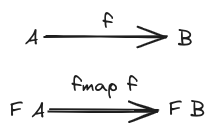
\includegraphics[width=0.3\textwidth]{figs/functor}
\end{figure}

\vocab{Контравариантный функтор} --- пара из типового конструктора и операции на функциях, разворачивающей стрелку.
Плюс соответствующие законы.

\begin{minted}{haskell}
    class Contravariant f where
      contramap :: (a -> b) -> (f b -> f a)
\end{minted}

\begin{figure}[H]
    \centering
    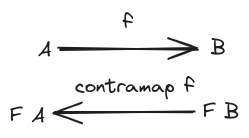
\includegraphics[width=0.3\textwidth]{figs/contra-functor}
\end{figure}

Типовой конструктор можно объявить ковариантным или контравариантным функтором (или никаким из них) относительно типового параметра в зависимости от вида декларации соответствующих конструкторов данных.
А именно, от \vocab{полярности}\footnote{\url{https://existentialtype.wordpress.com/2012/08/25/polarity-in-type-theory/}}\footnote{\url{https://ncatlab.org/nlab/show/polarity+in+type+theory}} позиций, в которых входит этот типовой параметр в декларации.

Попробуем развить интуитивное понимание полярностей.
Рассмотрим некоторое вычисление типа \texttt{F a}.
Параметр \texttt{a} входит в положительной позиции, если все его значения можно извлечь из \texttt{F a}, как в следующих примерах (для извлечения могут понадобиться паттерн-матчинг и аппликация):
\begin{minted}{haskell}
    data F a = L a | R a
    data F a = D a (Int -> a)
\end{minted}

Вхождения, наоборот, отрицательные, если значения соответствующего типа нельзя получить из вычисления, но нужно ему предоставить.
Например, в качестве параметров функций:
\begin{minted}{haskell}
    data F a = F (a -> Int)
    data F a = L (a -> ()) | R Int
\end{minted}
Действительно, для первого примера можно объявить инстанс \mintinline{haskell}|Contravariant|:
\begin{minted}{haskell}
    instance Contravariant F where
      contramap :: (a -> b) -> (F b -> F a)
      contramap g (F f) = F (f . g)
\end{minted}

Можно предположить, что на плюс и минус действуют обычные мультипликативные законы.
И это действительно так.
\begin{itemize}
    \item Плюс на плюс даёт плюс:
    \begin{minted}{haskell}
        data F a = F (Int -> (Int -> a))
    \end{minted}
    \item Плюс на минус (и наоборот) --- минус:
    \begin{minted}{haskell}
        data F a = F ((Int -> a) -> Int)
    \end{minted}
    \item Минус на минус --- плюс, поскольку параметр принимаемой функции выдаётся реализацией вызывающей стороне:
    \begin{minted}{haskell}
        data F a = F ((a -> Int) -> Int)
    \end{minted}
\end{itemize}

Тип от двух положительных параметров можно объявить \vocab{бифунктором}:
\begin{minted}{haskell}
    class Bifunctor f where
      bimap :: (a -> c) -> (b -> d) -> f a b -> f c d
\end{minted}

Тип от двух параметров, положительного и отрицательного, --- \vocab{профунктором}:
\begin{minted}{haskell}
    class Profunctor p where
      dimap :: (c -> a) -> (b -> d) -> p a b -> p c d
\end{minted}

Профункторы являются некоторыми обобщениями функциональной стрелки.
Например, если у нас есть SQL запрос, который по данным возвращает результат, его можно объявить профунктором с семантикой --- добавить пред-обработку входных данных и пост-обработку выходных:
\begin{minted}{haskell}
    dimap serialize deserialize (query :: Text -> Text) :: Age -> [User]
\end{minted}

Также понятие вариантности часто встречается в объектно ориентированных языках для обозначения возможности дополнить отношение подтипизации на полиморфные типы (да и вообще в теории подтипизации).

Действительно, \vocab{отношение подтипизации} \texttt{B <: A} говорит о том, что значение типа \texttt{B} безопасно использовать в позиции, где ожидается значение типа \texttt{A}.
Иначе говоря, существует функция \texttt{upcast :: B -> A}.
Если типовой конструктор \texttt{F a} ковариантен относительно параметра \texttt{a}, то по \texttt{upcast} найдётся \texttt{upcast' :: F B -> F A}.
То есть отношение подтипизации также автоматически включает \texttt{F B <: F A}.
Контравариантный случай аналогично.

\begin{task}
    Убедитесь в вашем любимом языке с поддержкой вариантности, что минус на минус даёт плюс.
\end{task}

\subsubsection{Data promotion \& kind polymorphism} \label{subsubsec:promotion}

Ранее мы программировали на уровне термов, а типы контролировали ``правильность'' построения термов.
Но типы так же являются языком как с синтаксической точки зрения, так и с вычислительной.
Вычисления на типах мы будем рассматривать далее, а в этом параграфе научимся конструировать в Haskell различные структуры на уровне типов.

В качестве модельной задачи зададим структуру данных, моделирующую вектор, но такую, что тип будет параметризован длиной.
Для начала определим натуральные числа на уровне типов в стиле Пеано:
\begin{minted}{haskell}
    data Zero
    data Suc n
\end{minted}

\begin{task}
    Сколько обитателей типа \mintinline{haskell}|Suc (Suc Zero)|?
\end{task}

Теперь мы можем задать тип вектора, содержащий информацию о длине:
\begin{minted}{haskell}
    data Vec (size :: Type) (elem :: Type) where
      VNil :: Vec Zero a
      VCons :: a -> Vec n a -> Vec (Suc n) a

    example :: Vec (Suc (Suc Zero)) Int
    example = VCons 1 (VCons 2 VNil)
\end{minted}

Для такого типа, например, можно написать безопасную функцию \mintinline{haskell}|zip|, работающую только на векторах одинаковой длины:
\begin{minted}{haskell}
    vzip :: Vec n a -> Vec n b -> Vec n (a, b)
    vzip VNil VNil = VNil                                      -- n ?$\sim$? Zero
    vzip (VCons x xs) (VCons y ys) = VCons (x, y) (vzip xs ys) -- n ?$\sim$? Suc n'
\end{minted}

Заметьте, что в остальных ветках \mintinline{haskell}|vzip| должны возникнуть эквивалентности, начинающиеся с различных конструкторов, например, \mintinline{haskell}|Zero ?$\sim$? Suc n|.
Поскольку невозможно построить такие аргументы функции, Haskell позволяет соответствующие ветки не рассматривать.

\begin{task}
    Напишите функцию добавления в конец элемента вектора.
    Двигайтесь последовательно, заполняя типовые дыры и отслеживая возникающие эквивалентности.
\end{task}

Удивительно, но сейчас наш язык типов не типизирован.
Действительно, кайнд \mintinline{haskell}|Suc| --- \mintinline{haskell}|Suc :: Type -> Type|, соответственно ничто не мешает написать \mintinline{haskell}|Suc (Maybe Int)|.
То есть язык кайндов, который должен контролировать типы, слишком беден.
В то же время он слишком ограничивающий, поскольку не поддерживает полиморфизм, что дало начало большому количеству дублирований а ля \mintinline{haskell}|Typeable (ty :: Type)|, \mintinline{haskell}|Typeable1 (ty :: Type -> Type)|\ldots

Чтобы обогатить систему кайндов для лучшего контроля за программами уровня типов, System $F_C$ была расширена до System $F_C^\uparrow$ (читается FC-pro)~\cite{yorgey2012giving}.
Это достигается автоматическим продвижением (promotion) \mintinline{haskell}|data| деклараций на уровень выше (расширение \href{https://downloads.haskell.org/ghc/latest/docs/users_guide/exts/data_kinds.html#extension-DataKinds}{DataKinds}).
А именно: любой конструктор типа также становится кайндом, а конструктор данных --- конструктором типа.
Так, в примере с числами, мы можем задекларировать натуральные числа как обычно и использовать на уровне типов:
\begin{minted}{haskell}
    data Nat = Zero | Suc Nat
    ghci> :k Suc :: Nat -> Nat
\end{minted}

Теперь вектору можно приписать более точный кайнд:
\begin{minted}{haskell}
    data Vec (size :: Nat) (elem :: Type) where
      VNil :: Vec Zero a
      VCons :: a -> Vec n a -> Vec (Suc n) a
\end{minted}

\begin{task}
    Что выведет \mintinline{haskell}|ghci> :k Vec|?
\end{task}

Поскольку типы и термы в Haskell живут в разных пространствах имён, можно называть конструкторы типов и данных одинаково.
Однако если продвинуть такой тип данных, возникнет неоднозначность: мы имеем в виду тип или продвинутый конструктор.
Haskell позволяет указать явно, что речь идёт о продвинутом конструкторе с помощью одинарной кавычки.
\begin{minted}{haskell}
    data T = T Nat
    ghci> :k T
    T :: Type      -- Речь про конструктор типа
    ghci> :k 'T
    'T :: Nat -> T -- Речь про продвинутый конструктор данных
\end{minted}

Недавние версии GHC поддерживают прямое объявление конструкций уровня типов с помощью расширения \href{https://downloads.haskell.org/ghc/latest/docs/users_guide/exts/type_data.html#extension-TypeData}{TypeData}.
Не любые \mintinline{haskell}|data| декларации подходят для продвижения, в то же время \mintinline{haskell}|type data| декларации позволяют явно запросить структуру уровня типов и получить внятные ошибки, если декларация написана неправильно.
\begin{minted}{haskell}
    type data Nat = Zero | Suc Nat
\end{minted}

В случае продвижения полиморфного типа, мы получаем полиморфные кайнды (\href{https://downloads.haskell.org/ghc/latest/docs/users_guide/exts/poly_kinds.html}{PolyKinds}):
\begin{minted}{haskell}
    data [a] = [] | (:) a [a]
    ghci> :k '(:)
    '(:) :: forall k . k -> [k] -> [k]
\end{minted}

\begin{figure}[h]
    \centering
    %! suppress = Quote
    \begin{tabular}{|c|c|c|}
        \hline
        Term                                   & Type                                            & Kind                                            \\
        \hline
        \mintinline{haskell}|Zero|             & \mintinline{haskell}|Nat|                       & \mintinline{haskell}|Type|                      \\
        \mintinline{haskell}|[Zero, Suc Zero]| & \mintinline{haskell}|[Nat]|                     & \mintinline{haskell}|Type|                      \\
        \mintinline{haskell}|[]|               & \mintinline{haskell}|forall a. [a]|             & \mintinline{haskell}|Type|                      \\
        \mintinline{haskell}|(:)|              & \mintinline{haskell}|forall a. a -> [a] -> [a]| & \mintinline{haskell}|Type|                      \\
        & \mintinline{haskell}|'Suc 'Zero|                & \mintinline{haskell}|Nat|                       \\
        & \mintinline{haskell}|'['Zero, 'Suc 'Zero]|      & \mintinline{haskell}|[Nat]|                     \\
        & \mintinline{haskell}|'[Int, Double]|            & \mintinline{haskell}|[Type]|                    \\
        & \mintinline{haskell}|'[]|                       & \mintinline{haskell}|forall k. [k]|             \\
        & \mintinline{haskell}|'(:)|                      & \mintinline{haskell}|forall k. k -> [k] -> [k]| \\
        \hline
    \end{tabular}
    \caption{Пример продвижений в Haskell.}
    \label{fig:universes}
\end{figure}

Примеры продвижения различных конструкций можно увидеть в таблице~\ref{fig:universes}.

Зададим гетерогенный список, индексированный типами элементов:
\begin{minted}{haskell}
    data HList (tys :: [Type]) where
      HNil :: HList '[]
      HCons :: ty -> HList tys -> HList (ty ': tys)

    example :: HList '[Int, Bool, Double]
    example = HCons 42 $ HCons True $ HCons 12.5 HNil
\end{minted}

Структуры данных тоже могут быть полиморфными по кайндам.
Рассмотрим следующий тип \href{https://hackage.haskell.org/package/tagged-0.8.8/docs/Data-Tagged.html#t:Tagged}{\mintinline{haskell}|Tagged|}, позволяющий дополнить тип значения дополнительным типовым тегом.
Кайнд тега может быть произвольным, поэтому, например, можем использовать встроенные в систему типов константы \href{https://ghc.gitlab.haskell.org/ghc/doc/users_guide/exts/type_literals.html}{TypeLits}:
\begin{minted}{haskell}
    newtype Tagged (tag :: k) (a :: Type) = Tagged a
    ghci> :t Tagged
    Tagged :: forall k (tag :: k) a. a -> Tagged tag a

    example :: Tagged ("hello" :: Symbol) Int
    example = Tagged 42
\end{minted}

Современный Haskell в итоге пришёл к тому, что система типов не делает различий между типами и кайндами (рис.~\ref{fig:types-eq-kinds}).
В частности, \mintinline{haskell}|Type :: Type|.
Это нужно для расширения возможностей Haskell в сторону программирования с зависимыми типами путём добавления несинтаксических эквивалентностей для кайндов (\href{https://ghc.gitlab.haskell.org/ghc/doc/users_guide/exts/poly_kinds.html#extension-TypeInType}{TypeInType}).
$System~FC$ была представлена в работе~\cite{weirich2013system}\footnote{\href{https://www.youtube.com/watch?v=ISGENChlA4M&list=PLvPsfYrGz3wufQguebnCduYgQQ9UMeJRt}{(youtube) Мини-курс на русском языке про развитие Haskell в сторону зависимой типизации.}}\footnote{\href{https://www.youtube.com/watch?v=_HYI7zjkrEs&list=PLvPsfYrGz3wuVAGhNf6-i7uafXg56oqM5&index=1}{(youtube) Мини-курс на русском языке --- система вывода типов Haskell.}}.

\begin{figure}[h]
    \centering
    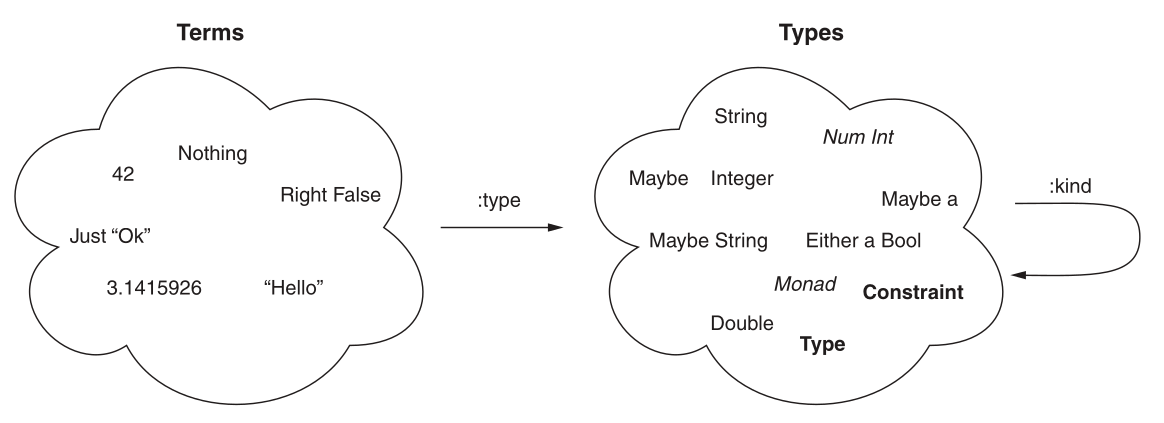
\includegraphics[width=0.99\textwidth]{figs/types-eq-kinds}
    \caption{Типы и канды --- одно~\cite{bragilevsky-haskell}.}
    \label{fig:types-eq-kinds}
\end{figure}

\subsection{Реализация параметрического полиморфизма}

\vocab{Конвенция вызова}\footnote{\url{https://en.wikipedia.org/wiki/Calling_convention}} представляет собой набор соглашений между тем, как функция компилируется и как должна вызываться.
Например, функция принимает два аргумента, каждый размером в машинное слово, и возвращает один результат размером в машинное слово.
Тогда сгенерированный низкоуровневый код этой функции может, например, ожидать, что оба аргумента передаются через специальную пару регистров, а складывать результат он будет в третий.
В таком случае вызывающий код обязан предоставить аргументы в правильных регистрах и ожидать результата в некотором третьем, заранее оговоренном регистре.

В общем случае, конвенция вызова функции зависит от типов аргументов и результата.
Нужно знать как минимум их размер, чтобы понять, размещать их в регистрах или на стеке.
Нужно знать, это указатель или значение само по себе, чтобы понимать, как с ним работать.

Таким образом, реализация параметрического полиморфизма в языке --- это не тривиальная задача.
Разные языки используют различные подходы, все со своими достоинствами и недостатками.

\subsubsection{Mономорфизация} \label{subsubsec:monomorphization}

\vocab{Mономорфизация} --- самый прямолинейный подход, компилируем функцию отдельно для каждого набора типовых аргументов.
Так, если различных наборов типовых аргументов, с которыми эта функция вызывается, например, 100 (что запросто может быть), то её код будет компилироваться сто раз и занимать в бинарнике в сто раз больше места.
Так делают, например, C++ и Rust.

На самом деле всё ещё хуже.
Если проект многомодульный и состоит из множества единиц компиляции (кусков, которые компилируются отдельно), то одна и та же специализация функции на типовые аргументы будет компилироваться заново во всех единицах компиляции, где такая специализация нужна.
А затем, линкер будет заниматься удалением дубликатов, что тоже не самый быстрый и эффективный процесс.

\begin{itemize}
    \item[\positive] Порождаемый код максимально эффективен для каждого типа;
    \item[\negative] Время компиляции крайне велико;
    \item[\negative] Существенно увеличивается размер результирующего бинарного файла, что может быть критично для некоторых приложений;
    \item[\negative] Может неэффективно работать из-за засорения кеша кода в процессоре;
    \item[\negative] В интерфейсах не может быть полиморфных методов, так как мы не знаем в месте вызова, к какому именно наследнику относится вызываемый метод, и какой код нужно специализировать;
    \item[\negative] К полиморфным функциям нельзя динамически линковаться (у них нет кода до специализации);
    \item[\negative] Нельзя поддержать variance, потому что код компилируется для конкретного типа и в общем случае не может работать для произвольного подтипа или супертипа.
\end{itemize}

Некоторые языки не делают инстанциацию скрытой деталью реализации языка, а предоставляют её как инструмент пользователям.
Так делают, например, C++ и Zig.
А именно, это позволяет добиться следующего:
\begin{itemize}
    \item Если разрешить использовать значения в типах, инстанциация может использоваться как механизм вычислений на этапе компиляции.
    \item Если отложить проверку ошибок на стадию инстанциирования, то мы получим своего рода статическую утиную типизацию.
    Это позволит не описывать сложные сигнатуры полиморфных функций.
    Однако тогда функции придётся вручную инстанциировать против всевозможных типов, иначе нельзя понять статически, компилируется она хотя бы против этих типов или нет.
\end{itemize}

% todo The Simple Essence of Monomorphization

\subsubsection{Стирание типа} \label{subsubsec:type-erasure}

Можно всё сделать наоборот, унифицировав значения, которые приходят на вход полиморфным функциям, вместо того, чтобы компилировать код под каждый тип.

Пусть каждое значение будет аллоцировано в куче и передаваться по указателю.
Тогда мы сможем переиспользовать один и тот же код для разных типовых аргументов, он просто будет ожидать указатели.

\begin{itemize}
    \item[\positive] Каждая функция компилируется ровно один раз --- быстро;
    \item[\positive] Можно динамически загружать новые полиморфные функции и типы и использовать их друг с другом;
    \item[\positive] Гибкость --- вариантность, полиморфные методы в интерфейсах, higher-ranked types\ldots просто работают;
    \item[\negative] Аллокация в куче и разыменование указателя может очень сильно замедлить код, особенно работающий с ``примитивными типами'';
    \item[\negative] Поскольку информация о типах стирается, нельзя ничего сделать с типовым аргументом, не имея его обитателей (например, запросить рефлексией информацию).
\end{itemize}

Такого подхода придерживаются JVM, Haskell и, как правило, другие функциональные языки ввиду его гибкости.

Особую проблему вызывает работа с примитивами, потому что каждое значение приходится сначала боксить (переносить в кучу), а потом уже использовать в полиморфном контексте.
Поэтому языки борются с этим как могут.
Некоторые языки урезают диапазоны значений примитивов, чтобы зарезервировать бит, определяющий, это указатель или значение.
Код консультируется с этим битом для работы (похоже на~\ref{subsubsec:swift-generics}).
Так делают, например, OCaml и \href{https://koka-lang.github.io/koka/doc/book.html#sec-value-types}{Koka}.
Агрессивный инлайнинг тоже помогает.
Java пытается аккуратно двигаться в сторону возможности мономорфизации\footnote{\href{https://youtu.be/JI09cs2yUgY?si=MLkRs31mN1koXIu1}{Type Specialization of Java Generics - What If Casts Have Teeth ?}}\footnote{\url{https://cr.openjdk.org/~jrose/values/parametric-vm.html}}.

\subsubsection{Гибридный подход} \label{subsubsec:hybrid}

С\# реализует гибридный подход\footnote{\href{https://learn.microsoft.com/en-us/dotnet/csharp/programming-guide/generics/generics-in-the-run-time}{Generics in the runtime (C\# programming guide).}}.
Они различают значения, хранимые в куче --- \vocab{reference types}, и значения, хранимые на стеке --- \vocab{value types}.
Для первых они генерируют одну специализацию, работающую с указателями.
Для каждого набора value-типов они генерируют лениво в рантайме специализацию.

То есть следы дженериков в таком подходе есть в промежуточном представлении CIL, а также в рантайме.

\begin{itemize}
    \item[\positive] Порождается эффективный код, работающий с примитивами;
    \item[\positive] Доступна рефлексия по дженерикам;
    \item[\positive] Небольшое время компиляции;
    \item[\negative] Инстанциация в рантайме замедляет исполнение;
    \item[\negative] Variance работает только для reference types (что странно --- есть ``правильная'' подтипизация, а есть ``неправильная'').
\end{itemize}

% todo выпросить инфу про подтипизацию у Михаила

\subsubsection{Использование виртуальной таблицы свойств типов} \label{subsubsec:swift-generics}

Swift\footnote{\href{https://youtu.be/ctS8FzqcRug?si=y_ZYnuUOulA33d_X}{(youtube) 2017 LLVM Developers’ Meeting: ``Implementing Swift Generics''}} вместе с каждым типовым параметром передаёт value witness table (рис.~\ref{fig:swift-witness-table}).
Это таблица со всей необходимой информацией, о типе: размер и выравнивание, что нужно сделать при копировании и перемещении объекта (например, инкрементировать счётчик ссылок).
Таким образом, скомпилированный код постоянно обращается к этой таблице и делает виртуальные вызовы функций из неё (рис.~\ref{fig:swift-generated-code}).
\begin{figure}[h]
    \centering
    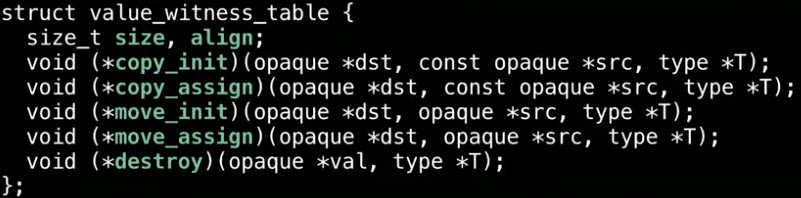
\includegraphics[width=0.7\textwidth]{figs/swift-witness-table}
    \caption{Swift value witness table.}
    \label{fig:swift-witness-table}
\end{figure}
\begin{figure}[h]
    \centering
    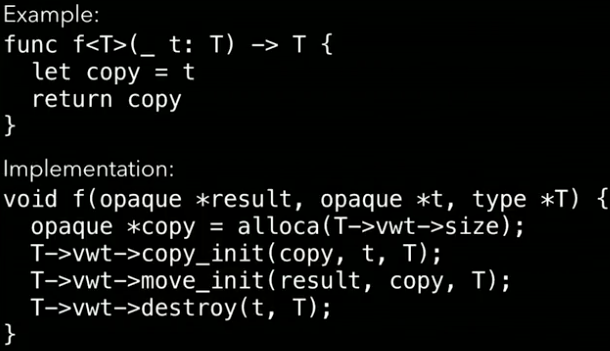
\includegraphics[width=0.6\textwidth]{figs/swift-generated-code}
    \caption{Код полиморфной функции, порождаемый компилятором Swift.}
    \label{fig:swift-generated-code}
\end{figure}

\begin{itemize}
    \item[\positive] Небольшое время компиляции;
    \item[\positive] Предсказуемая эффективность (не приводит к неожиданным паузам в рантайме);
    \item[\positive] Эффективная работа с value-значениями;
    \item[\positive] Высокая гибкость;
    \item[\positive] Информация о типах не стирается;
    \item[\negative] Серьёзный константный оверхед на динамические вызовы через таблицу, эффективность очень сильно зависит от компиляторных оптимизаций.
\end{itemize}

Своего рода реализация параметрического полиморфизма через специальный.

\subsection{Полиморфизм по конвенции вызова} \label{subsec:representation-polymorphism}

Как мы уже обсуждали выше~\ref{subsubsec:type-erasure}, параметрический полиморфизм в Haskell реализуется следующим образом: все значения хранятся в куче и передаются в полиморфные функции по указателю.
Однако, если для вычислительного кода важна производительность, такой подход не годится ввиду большой нагрузки на подсистему управления памятью и множества индирекций.
Поэтому Haskell позволяет также писать код с использованием unboxed значений.
А если конвенция вызова не принципиальна, можно по ней абстрагироваться и писать один код для boxed и unboxed значений~\cite{eisenberg2017levity}.

\subsubsection{Классификация значений по runtime представлению}

\begin{figure}[h]
    \centering
    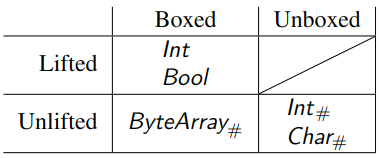
\includegraphics[width=0.5\textwidth]{figs/haskell-value-kinds}
    \caption{Виды значений в Haskell с примерами~\cite{eisenberg2017levity}.}
    \label{fig:haskell-value-kinds}
\end{figure}

На рисунке~\ref{fig:haskell-value-kinds} можно увидеть классификацию значений в Haskell с примерами типов.
\vocab{Unboxed типы} --- их значения удерживаются и передаются по значению.
\vocab{Boxed}, соответственно, наоборот, передаются по указателю и хранятся в куче.
Обычный \mintinline{haskell}|Int| является просто декларацией следующего вида, где \mintinline{haskell}|I#| --- это обычный конструктор с необычным именем, содержащий unboxed значение.
\begin{minted}{haskell}
    data Int = I# Int#
\end{minted}

\vocab{Lifted типы} --- содержат $\bot$ в качестве значения.
Иначе говоря, могут содержать отложенные вычисления.
\vocab{Unlifted типы} --- наоборот, не могут быть отложенными.
Операции, производящие значения unlifted типов всегда энергичные.
Свойство lifted/unlifted называют \vocab{levity}.
Чтобы распространить дальнейшее изложение на энергичные языки, можно levity заменить на boxity и всё останется справедливым.

\# в именах типов и функций --- это конвенция, показывающая, что где-то рядом происходит работа с unlifted значениями\footnote{Нужно подключить расширение \href{https://ghc.gitlab.haskell.org/ghc/doc/users_guide/exts/magic_hash.html}{MagicHash}, чтобы пользоваться \# в идентификаторах.}.

Также в Haskell есть unboxed кортежи, которых не существует на этапе исполнения.
Например, следующая функция как бы возвращает пару значений, но в действительности компилятор может их разместить, например, в паре регистров.
Соответственно, паттерн-матчинг по таким кортежам, просто позволяет сослаться на каждое из этих значений.
\begin{minted}{haskell}
    divMod# :: Int -> Int -> (# Int, Int #)
    case divMod# n k of (# quot, rem #) -> ...
\end{minted}
Соответственно, нет никакого различия между по-разному вложенными unboxed кортежами:
\begin{minted}{haskell}
    (# A, (# B, C #)) ?$\equiv$? (# #( A, B #), C #) ?$\equiv$? (# A, B, C #)
\end{minted}

\subsubsection{Representation polymorphism}

Значения различных типов могут быть на этапе исполнения устроены по-разному.
То есть нам нужна некоторая система классификации типов.
Но такая система в Haskell уж есть --- кайнды.
Опишем в виде структур данных предметную область, а потом продвинем на нужный уровень с помощью DataKinds~\ref{subsubsec:promotion}.

Стандартная библиотека Haskell \href{https://downloads.haskell.org/ghc/latest/docs/users_guide/exts/representation_polymorphism.html}{предоставляет} следующие типы данных:
\begin{minted}{haskell}
    TYPE :: RuntimeRep -> Type

    data Levity = Lifted | Unlifted

    data RuntimeRep = BoxedRep Levity
                    | IntRep | DoubleRep
                    | TupleRep [RuntimeRep]
                    | SumRep [RuntimeRep]
                    | ...

    type LiftedRep = BoxedRep Lifted

    type Type = TYPE LiftedRep
\end{minted}

\mintinline{haskell}|TYPE| --- это магический тип, определённый в компиляторе.
Он параметризован runtime-представлением значений.
Теперь привычный \mintinline{haskell}|Type| --- это частный случай с boxed lifted значениями.

%! suppress = Quote
\begin{itemize}
    \item \mintinline{haskell}|Int :: TYPE (BoxedRep Lifted)| или \mintinline{haskell}|:: Type|
    \item \mintinline{haskell}|IntRep| и \mintinline{haskell}|DoubleRep| соответствуют представлению численных констант (в зависимости от архитектуры процессора, целые числа и числа с плавающей запятой может быть необходимо располагать в различных специальных регистрах)\\ \mintinline{haskell}|Int# :: TYPE IntRep|
    \item \mintinline{haskell}|Maybe Int :: Type|
    \item \mintinline{haskell}|Maybe :: Type -> Type|
    \item \mintinline{haskell}|TupleRep| и \mintinline{haskell}|SumRep| --- unboxed алгебраические типы, представления параметризованы представлениями хранимых значений\\
    \mintinline{haskell}|(# Int, Bool #) :: TYPE (TupleRep '[LiftedRep, LiftedRep])|
    \item Для простоты не унифицируются типы вложенных кортежей
    \begin{minted}{haskell}
        (# Int#, (# Int, Double# #) #)
          :: TYPE (TupleRep '[IntRep, TupleRep '[LiftedRep, DoubleRep]])
    \end{minted}
\end{itemize}

Выставив runtime-представление в структуре кайндов, мы теперь можем параметризоваться по ним.
Например, кайнд функциональной стрелки выглядит следующим образом\footnote{Выключить упрощения: \mintinline{haskell}|ghci> :set -fprint-explicit-foralls -fprint-explicit-runtime-reps|}:
\begin{minted}{haskell}
    ghci> :k (->)
    (->) :: forall {q :: RuntimeRep} {r :: RuntimeRep}. TYPE q -> TYPE r -> Type
\end{minted}

К сожалению, Haskell выставляет довольно строгое ограничение: связыватели не могут иметь тип, полиморфный по runtime представлению.
Можно легко предположить, почему, --- нельзя сгенерировать код функции для работы с параметром произвольного рантайм-представления.
Это можно решить только мономорфизацией~\ref{subsubsec:monomorphization}, но Haskell избегает этого подхода\footnote{\url{https://gitlab.haskell.org/ghc/ghc/-/issues/14917}}.
Сообщество также пытается найти другие решения\footnote{\url{https://mail.haskell.org/pipermail/haskell-cafe/2023-January/135770.html}} (что-то вроде~\ref{subsubsec:swift-generics}).

Например, изначально оператор аппликации был обобщён только по возвращаемому типу.
Это не порождает проблем, так как вызывающий код сможет вывести представление и сгенерировать подходящий код:
\begin{minted}{haskell}
    ($) :: forall r a (b :: TYPE r). (a -> b) -> a -> b
    f $ ?\framebox{x}? = f x
\end{minted}

Однако, было замечено, что для оператора аппликации можно получить другую реализацию, не использующую levity-полиморфное связывание\footnote{\url{https://gitlab.haskell.org/ghc/ghc/-/merge_requests/10131}}:
\begin{minted}{haskell}
    ($) :: forall ra rb (a :: TYPE ra) (b :: TYPE rb). (a -> b) -> a -> b
    ($) f = f
\end{minted}


% todo haskell and ST-trick https://link.springer.com/article/10.1007/BF01018827


    \clearpage


    \section{Специальный (ad-hoc) полиморфизм} \label{sec:ad-hoc}

    %! suppress = MissingLabel

Как-то Joe Fasel в разговоре с Philip Wadler высказал идею того, что перегрузка функций (overloading) должна находить своё отражение в типах.
Wadler понял его неправильно~\cite{hudak2007history}.
Но то, что он понял, --- оказалось классами типов~\cite{wadler1989make}.

Christopher Strachey ввёл классификацию полиморфизма на две категории.
Параметрический --- один и тот же код работает с данными различных типов.
\vocab{Специальный (ad-hoc) полиморфизм} --- код выбирается в зависимости от типа.
Например, один и тот же символ умножения по-разному действует на целые числа и на числа с плавающей точкой.

Перегрузка в языках обозначает возможность назвать несколько функций одинаково, у которых должны быть различные наборы входных параметров.
В месте вызова компилятор статически определяет по типам аргументов, какую из них действительно следует вызвать.
\begin{minted}{cpp}
    string toString(x: int) { ... }
    string toString(fmt: String, d: double) { ... }
\end{minted}

Классы типов обязуют сначала задекларировать именованную сущность (собственно, класс типов), которая включает в себя пачку деклараций функций, которые могут быть перегружены для различных типов.
\begin{minted}{haskell}
    class Show a where
      show :: a -> String

    instance Show Int where
      show :: Int -> String
      show = ...
\end{minted}

Необходимо заметить, что декларация класса типов содержит формальный типовой параметр, по вхождениям которого в тип функции, собственно, выбирается перегрузка.
Таких параметров может быть много, они могут иметь стрелочные кайнды.
Например, в случае класса типов \mintinline{haskell}|Applicative|, выбор реализации операции \mintinline{haskell}|pure| будет происходить по типовому конструктору результата, то есть даже не по полноценному типу.
Такая гибкость и близко не достигается при классической перегрузке.
\begin{minted}{haskell}
    class Functor f => Applicative (f :: Type -> Type) where
      pure :: a -> f a
      ...

    instance Applicative Maybe where
      pure :: a -> Maybe a
      ...
\end{minted}

Также, в отличие от перегрузки, классы типов совместимы с параметрическим полиморфизмом.
Так, в типе полиморфной функции нельзя указать, что для типа должна присутствовать определённая перегрузка.
Классы типов же позволяют ограничить набор возможных типовых аргументов теми, для которых реализован инстанс нужного класса типов:
\begin{minted}{haskell}
    showPrefixed :: Show a => a -> String -> String
\end{minted}

Если сравнивать классы типов с переопределением (overriding) в ООП языках, то разрешение вызова виртуальной функции происходит с использованием таблицы, хранящейся объекте первого параметра (получателя вызова, receiver).
Классы типов же опираются исключительно на тип, поэтому, например, возможно определение констант в классах типов:
\begin{minted}{haskell}
    class Enum a => Bounded a where
      minBound :: a
      maxBound :: a
\end{minted}

В то же время, классы типов не являются типами, а, скорее, предикатами на типах.
Тип удовлетворяет такому предикату, или свойству, если для него есть соответствующий инстанс.
Поэтому, в частности, привычный способ в ООП создать гетерогенную коллекцию элементов, имеющих общий интерфейс, напрямую не сработает с классами типов.
Например, такой тип не будет корректным: \mintinline{haskell}|[Show]|.
Мы вернёмся к этой проблеме в~\ref{subsubsec:existentials}.

\subsection{Устройство классов типов}

Несмотря на поразительное могущество, идея реализации классов типов крайне проста.
Она была уже во всей полноте представлена в первой работе~\cite{wadler1989make}.
В дальнейших работах уточнялся механизм вывода типов в виде сведения к классической системе типов в стиле Hindley-Milner~\cite{hall1996type}.
Остальные работы, в основном, предлагают огромное разнообразие различных приложений.

\subsubsection{Словари}

Рассмотрим идею реализации классов типов на примере полиморфной сортировки.
Сортировка для списка элементов конкретного типа пишется тривиально:
\begin{minted}{haskell}
    sort :: [Int] -> [Int]
    sort = \case [] -> []; x:xs -> insert x (sort xs)
      where
        insert x xs = let (l, r) = List.partition (?\framebox{<}? x) xs in l ++ x : r)
\end{minted}

В реализации единственная информация о типе, которой мы пользуемся --- порядок на его обитателях.
Таким образом, при переходе к полиморфной сортировке, нам нужно принять словарь с предикатами, задающими нужный порядок для данного типа\footnote{Приятный синтаксис распаковки рекордов доступен с расширением \href{https://ghc.gitlab.haskell.org/ghc/doc/users_guide/exts/record_wildcards.html}{RecordWildCards}.}.
\begin{minted}{haskell}
    data OrdDict a = OrdDict { less :: a -> a -> Bool }

    sort :: OrdDict a -> [a] -> [a]
    sort d@OrdDict {..} = \case [] -> []; x:xs -> insert x (sort d xs)
      where
        insert x xs = let (l, r) = List.partition (?\framebox{`less`}? x) xs in l ++ x : r)
\end{minted}

Теперь, чтобы воспользоваться сортировкой на списке чисел, нужно сконструировать нужный рекорд и вызвать с ним функцию на списке конкретных типов:
\begin{minted}{haskell}
    intOrd :: OrdDict Int
    intOrd = OrdDict { less = (<) }

    ghci> sort intOrd [3, 2, 1]
\end{minted}

Возможна ситуация, когда инстанс для одного типа зависит от инстанса для другого
Например, сравнение списков можно получить автоматически, зная порядок на элементах.
В случае словарей мы это моделируем функцией между словарями:
\begin{minted}{haskell}
    listDict :: OrdDict a -> OrdDict [a]
    listDict d = OrdDict { less = ... ?\framebox{less d}? ... }
\end{minted}

Теперь мы можем сортировать список списков, конструируя нужный словарь:
\begin{minted}{haskell}
    ghci> sort (listDict intDict) [[3, 2], [2, 1], [0]]
\end{minted}

Сравнение явной передачи словарей и классов типов можно увидеть в следующей таблице:

\begin{tabular}{p{8cm}p{8cm}}
    \begin{enumerate}
        \item Определение словаря функций
        \begin{minted}{haskell}
            data MyOrd a = MyOrd
              { less :: a -> a -> Bool }
        \end{minted}
        \item Экземпляр словаря для конкретного типа
        \begin{itemize}
            \item Именованное значение
        \end{itemize}
        \begin{minted}{haskell}
            intMyOrd :: MyOrd Int
            intMyOrd = MyOrd { less = (<) }
        \end{minted}
        \item Явный параметр функции
        \begin{minted}{haskell}
            sort :: MyOrd a -> [a] -> [a]
        \end{minted}
        \item Передаётся пользователем
        \begin{minted}{haskell}
            test = sort ?\framebox{intMyOrd}? [3, 2, 1]
        \end{minted}
    \end{enumerate}
    &
    \begin{enumerate}
        \item Определение класса типов
        \begin{minted}{haskell}
             class MyOrd a where
               less :: a -> a -> Bool
        \end{minted}
        \item Объявление типа представителем класса типов
        \begin{itemize}
            \item Не имеет имени
        \end{itemize}
        \begin{minted}{haskell}
            instance MyOrd Int where
              less = (<)
        \end{minted}
        \item Неявный параметр функции
        \begin{minted}{haskell}
            sort :: MyOrd a => [a] -> [a]
        \end{minted}
        \item Передаётся компилятором
        \begin{minted}{haskell}
            test = sort [3, 2, 1]
        \end{minted}
    \end{enumerate}
\end{tabular}

Таким образом, словарь --- это свидетель (witness) того, что тип удовлетворяет ограничению.
Подобно тому, как коерции свидетельствуют несинтаксические эквивалентности на типах~\ref{subsubsec:gadts}.

\begin{task}
    Какой словарь будет соответствовать higher-kinded классу типов \mintinline{haskell}|Functor|?
\end{task}

\subsubsection{Неявные аргументы}

Можно думать так, что слева от \mintinline{haskell}|=>| передаются неявные аргументы функций, выводимые компилятором из контекста.
То есть, например, не стоит удивляться вхождениям \mintinline{haskell}|=>| в отрицательной позиции, это просто функция с неявным аргументом.
Так, следующий код не скомпилируется, потому что в месте использования переменной \texttt{y} нет значения типа \mintinline{haskell}|Show b|:
\begin{minted}{haskell}
    f :: (Show b => b) -> b
    f x = ?\framebox{x}?
\end{minted}
Можно это значение принять в функции \texttt{f}, тогда оно автоматически пропагируется в \texttt{y}:
\begin{minted}{haskell}
    f :: Show b => (Show b => b) -> b
    f x = ?\framebox{x}?
\end{minted}

Расширение \href{https://ghc.gitlab.haskell.org/ghc/doc/users_guide/exts/implicit_parameters.html}{ImplicitParams} даёт возможность делать некоторое аргументы функции неявными.
Фактически, это реализация динамического связывания в статическом языке~\cite{lewis2000implicit}.
Неявные аргументы берутся из скоупа по имени и подставляются автоматически:
\begin{minted}[escapeinside=##]{haskell}
    sortBy :: (a -> a -> Bool) -> [a] -> [a]

    sort :: (?cmp :: a -> a -> Bool) => [a] -> [a]
    sort = sortBy ?cmp
\end{minted}

Haskell также предоставляет возможность сохранять словари в структуры данных:
\begin{minted}{haskell}
    data ShowDict a where
      ShowDict :: Show a => ShowDict a

    f :: ShowDict b -> (Show b => b) -> b
    f d x = case d of ShowDict -> ?\framebox{x}? -- в скоупе доступен инстанс Show b
\end{minted}

\subsubsection{Вывод инстансов}

Чтобы вызвать ограниченно-полиморфную функцию, GHC производит вывод инстансов или, иначе говоря, автоматически конструирует свидетелей.
Вывод инстансов тесно интегрирован с общей системой вывода типов Haskell~\cite{spj-type-inference}.

В действительности вывод инстансов это не что иное, как \point{задача населения типа}.
Действительно, после трансляции в Core (промежуточное представление в GHC), классы типов представляют собой словари функций.
У нас в контексте имеются конкретные словари и функции, позволяющие из одних словарей получать другие.
Требуется найти терм, конструирующий словарь нужного типа.

Например, внутри функции \mintinline{haskell}|f :: Show a => ..| происходит вызов ограниченно- полиморфной функции
\mintinline{haskell}|g :: Show [a] -> ..|.
У нас имеется словарь \mintinline{haskell}|ShowDict a|, а так же функция \mintinline{haskell}|ShowDict a -> ShowDict [a]|, пришедшая из импортов\footnote{Инстансы можно импортировать пустым импортом: \mintinline{haskell}|import Module ()|.}.
Необходимо сконструировать терм типа \mintinline{haskell}|ShowDict [a]|.
Очевидно, это будет просто аппликации одного к другому.

Вывод инстансов происходит рекурсивно.
Чтобы вывести \mintinline{haskell}|ShowDict [a]|, выводится сначала посылка \mintinline{haskell}|ShowDict a|.
То есть получается рекурсия по структуре типа.
Иначе говоря, вывод инстансов можно эксплуатировать как вычислительный примитив уровня типов.
Так, например, мы можем опускать информацию из типов в термы:
\begin{minted}{haskell}
    type data Nat = Zero | Suc Nat

    class KnownNat (n :: Nat) where
      natVal :: Int

    instance KnownNat Zero where
      natVal = 0

    instance KnownNat n => KnownNat (Suc n) where
      natVal = 1 + natVal @n

    ghci> natVal @(Suc (Suc Zero))
    -- выведется natVal {knownSuc (knownSuc knownZero)}
\end{minted}

В общем случае процесс населения типа, как можно предположить по вычислительной аналогии, неразрешим.
Поэтому GHC накладывает большое количество ограничений на вид инстансов, которые гарантируют тотальность вывода.
Подробно эти ограничения описаны в~\cite{sulzmann2007understanding}.
Также GHC предоставляет различные расширения, ослабляющие эти ограничения и перекладывающие часть ответственности на плечи программиста\footnote{\url{https://downloads.haskell.org/ghc/latest/docs/users_guide/exts/instances.html}}.
Например, c UndecidableInstances можно легко написать разворот списка типов на этапе компиляции, как и любую другую функцию:
\begin{minted}{haskell}
    class Reverse (acc :: [Type]) (tys :: [Type]) where
      showReverse :: String

    instance ShowT acc => Reverse acc '[] where
      showReverse = showTypes @acc

    instance Reverse (ty : acc) tys => Reverse acc (ty : tys) where
      showReverse = showReverse @(ty : acc) @tys

    ghci> showReverse @'[] @'[Char, Int, Double]
\end{minted}

Вывод инстансов опирается только на вид "головы" декларации --- справа от \mintinline{haskell}|=>|, а ограничения слева применяются постфактум.
Это можно использовать, чтобы писать более общие инстансы.
Так, например, работает \vocab{constraint trick}\footnote{\url{https://chrisdone.com/posts/haskell-constraint-trick/}}, позволяющий резолвить ad-hoc полиморфные функции в параметрически-полиморфном контексте.

Этим же пользуется механизм программируемых ошибок компиляции из \href{https://hackage.haskell.org/package/base-4.20.0.1/docs/GHC-TypeLits.html}{GHC.TypeLits}.
Если инстанс сработал и компилятор начал обрабатывать ограничения слева, значит, что-то пошло не так~\cite[глава 12]{maguire-types}.

\begin{minted}{haskell}
    instance (TypeError
      ( Text "Attempting to show a function of type "
        :<>: Text "'" :<>: ShowType (a -> b) :<>: Text "'"
        :$$: Text "Did you forget to apply an argument?"
      )) => Show (a -> b) where
      show = undefined -- реализация не важна, до исполнения дело не дойдёт
\end{minted}

\subsubsection{Построение типа по значению}

После того как мы научились опускать значения из типов, закономерно научиться обратному --- поднимать значения в типы.

Рассмотрим вспомогательную концепцию проксирования.
В стандартной библиотеке определён тип \mintinline{haskell}|Proxy| с одним фантомным параметром.
Исторически он нужен, чтобы обходить отсутствие расширений \href{https://downloads.haskell.org/ghc/latest/docs/users_guide/exts/type_applications.html#extension-TypeApplications}{TypeApplications} и \href{https://downloads.haskell.org/ghc/latest/docs/users_guide/exts/type_abstractions.html#extension-TypeAbstractions}{TypeAbstractions}.
А именно --- неинформативную константу \mintinline{haskell}|Proxy| можно проаннотировать нужным типом и передать в функцию, чтобы специализировать типовой параметр на нужный тип.
Или принять \mintinline{haskell}|Proxy| и воспользоваться \href{https://downloads.haskell.org/ghc/latest/docs/users_guide/exts/scoped_type_variables.html#pattern-type-signatures}{ScopedTypeVariables} для типовых сигнатур в паттернах.
\begin{minted}{haskell}
    data Proxy (a :: k) = Proxy

    id :: Proxy a -> a -> a
    ghci> :t id (Proxy :: Proxy Int)
    id (Proxy :: Proxy Int) :: Int -> Int

    id (Proxy :: Proxy ?\framebox{a}?) x = (x :: ?\framebox{a}?)
\end{minted}

Иногда прокси-тип оставляют полиморфным, чтобы пользователь сам мог его задать.
Вместо конкретного значения иногда передают специализированное значение $\bot$, а получатель, не зная тип, не сможет его форсировать (однако, любые вхождения $\bot$ в тип слишком настораживают).
\begin{minted}{haskell}
    id :: proxy a -> a -> a
    id (_ :: proxy a) x = (x :: a)

    ghci> :t id (undefined :: Proxy Int)
    id (undefined :: Proxy Int) :: Int -> Int
\end{minted}

Теперь напишем функцию поднятия значения в тип с помощью техники через полиморфную рекурсию, описанную, например, в~\cite{kiselyov2004functional}.

В действительности мы, конечно, не можем честно получить синтаксически тип нужного размера, просто потому, что типы существуют строго до стадии исполнения.
Однако, как мы знаем, словари классов типов имеют воплощение в рантайме (случай полиморфной рекурсии~--- как раз пример, когда этого нельзя полностью избежать).
Поэтому воспользуемся continuation passing style, который будет подробно рассмотрен в главе~\ref{sec:continuations}: вместо того, чтобы вернуть результат, примем продолжение, умеющее работать с любым типом с \mintinline{haskell}|KnownNat|:
\begin{minted}{haskell}
    reify :: Int -> (forall n. KnownNat n => Proxy n -> a) -> a
    reify n k
      | n <= 0 = k (Proxy @Zero)
      | otherwise = reify (n - 1) \(Proxy :: Proxy n) -> k (Proxy @(Suc n))
\end{minted}

Продолжение, передаваемое в рекурсивный вызов, неявно принимает словарь для типа \texttt{n} и конструирует словарь для \mintinline{haskell}|Suc n|.

Наконец, можем написать следующую удивительную тождественную функцию, поднимающую сначала значение в тип, а потом опускающее тип обратно в термы:
\begin{minted}{haskell}
    wonderId :: Int -> Int
    wonderId n = reify n (\(Proxy :: Proxy n) -> natVal @n)
\end{minted}

\subsubsection{Имплиситы и когерентность}

Существуют подходы к реализации классов типов, когда они не являются отдельной возможностью языка, а получаются как следствие других, более общих, механизмов.

Так, в Scala существует механизм имплиситов (implicits)~\cite{kvrikava2019scala}.
Параметры функции могут быть помечены \mintinline{scala}|implicit|.
Теперь, если в контексте есть \mintinline{scala}|implicit| значения и \mintinline{scala}|implicit| функции, аргументы сгенерируются автоматически исходя из типа параметра.
Теперь мы можем смоделировать словарь функций, например, с помощью интерфейсов (которые в Scala называются \mintinline{scala}|trait|) и синглтонов, чтобы получить вполне себе классы типов~\cite{oliveira2010type}.
Функции с имплисит-параметрами не являются в полном смысле функциями первого класса в Scala.
\begin{minted}{scala}
    trait Show[T] {
        def show(x: T): String
    }

    def show[T](x: T)(implicit ev: Show[T]): String = ev.show(x)

    implicit object intShow extends Show[Int] {
        def show(x: Int): String = x.toString
    }

    def showAll[T](xs: List[T])(implicit ev: Show[T]): String =
        xs.map(show(_)).join(", ")
\end{minted}

В языках с зависимыми типами неявные параметры\footnote{\url{https://agda.readthedocs.io/en/v2.7.0.1/language/implicit-arguments.html}} особенно нужны, потому что, например, типы --- это такие же параметры функции, как и все остальные.
Поэтому вывод типов~--- это фактически вывод неявных аргументов функций.
Более того, зависимые функции, вместе с аргументами часто принимают доказательства каких-то свойств этих аргументов, которые тоже хочется по возможности выводить из контекста автоматически.
В свете аналогии между классами типов как предикатами на типах, а инстансами как доказательствами, свидетельствующими о выполнении предиката для типа, можно тот же механизм вывода доказательств переиспользовать для эмулирования классов типов\footnote{\url{https://agda.readthedocs.io/en/v2.7.0.1/language/instance-arguments.html}}~\cite{devriese2011bright}.
В обратную сторону можно механизмы зависимой типизации эмулировать классами типов~\cite{mcbride2002faking}.

Выражение классов типов через другие механизмы может выглядеть как абсолютно выигрышная стратегия на фоне реализации их как самостоятельной возможности языка.
Действительно, можно переиспользовать всё то могущество программирования, которое есть с рекордами, в то время как для классов типов и констреинтов то же самое приходится развивать отдельно\footnote{\url{https://downloads.haskell.org/ghc/latest/docs/users_guide/exts/instances.html}}.
Да и неявные аргументы, наверное, полезный механизм сам по себе.

Однако у подхода Haskell есть важное свойство при соблюдении всех ограничений, т.е. при отсутствии \vocab{orphan instances}\footnote{\url{https://stackoverflow.com/questions/3079537/orphaned-instances-in-haskell}}.
\vocab{Когерентность инстансов (coherence)} --- для одного типа все инстансы данного класса типов, полученные разными способами, неотличимы (рис.~\ref{fig:coherence}).
Соответственно, не имеет значения происхождение того или иного инстанса.
Иначе говоря, об этом можно не думать, это снимает существенное количество когнитивной нагрузки и упрощает рефакторинг\footnote{\href{https://youtu.be/hIZxTQP1ifo?si=aG2Lk2eb-5E5SOLb}{Edward Kmett - Type Classes vs. the World.}}.
В то время как остальные подходы требуют трепетного отношения к контексту вызова, потому что из него может прийти неожиданная реализация.

\begin{figure}
    \centering
    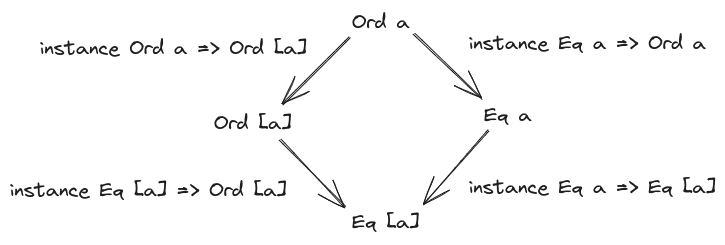
\includegraphics[width=0.8\linewidth]{figs/coherence}
    \caption{Когерентность инстансов --- диаграмма коммутирует.}
    \label{fig:coherence}
\end{figure}

\subsubsection{Правила (rules) и специализация}

GHC позволяет прямо в коде, с помощью специально прагмы, указывать оптимизирующие правила переписывания для компилятора\footnote{\url{https://downloads.haskell.org/ghc/latest/docs/users_guide/exts/rewrite_rules.html}}.
Например:
\begin{minted}{haskell}
    {-# RULES
      "map/map"    forall f g xs.  map f (map g xs) = map (f . g) xs
      "map/append" forall f xs ys. map f (xs ++ ys) = map f xs ++ map f ys
     #-}
\end{minted}

В частности, можно переписать полиморфную версию функции на специализированную, если типы подходят.
Для этого нужно реализовать специализированную версию (совпадение семантики --- полностью ответственность программиста) и задать соответствующее правило переписывания:
\begin{minted}{haskell}
    genericLookup :: Ord a => Table a b   -> a   -> b
    intLookup     ::          Table Int b -> Int -> b

    {-# RULES "genericLookup/Int" genericLookup = intLookup #-}
\end{minted}

Основной эффект такой оптимизации --- гарантированное превращение динамических вызовов функций классов типов в статические (потому что тип известен, следовательно, --- и соответствующий ему словарь).

\subsection{Семейства, ассоциированные семейства}

% todo fist-class type families

% todo \chapter*{FunWithTypeFuns}

% todo

\subsection{Кайнд Constraint}






\cite{constraint-kind}

% todo vadics example

% todo tuple constraints

% todo constraint families and constraint synonims

% todo https://downloads.haskell.org/ghc/latest/docs/users_guide/exts/quantified_constraints.html

% todo с constraint kinds фигня отсюда не нужна Haskell Type Constraints Unleashed

\cite{orchard2010haskell}

% todo

\subsection{Использование классов типов}

% todo

\subsubsection{Сериализация}

% todo

\subsubsection{Рефлексия на типах}

\cite{peyton2016reflection}

% todo

\subsubsection{Экзистенциальные типы} \label{subsubsec:existentials}

\cite[глава 7]{maguire-types}

% todo dynamic

% todo

\subsubsection{Получение значений с уровня типов}

% todo

\subsubsection{Коерции}

\cite{breitner2014safe}

\cite[глава 8]{maguire-types}

% todo type roles


% todo what do you want to give name to


% todo constraint is a proposition and dict is a proof

% todo constraints package of Edward Kmett

% todo monomorphism restriction

% todo pattern-matching on types

% todo serializer and serializable

% todo proxy

% todo algebra driven design

% todo rules and coersion

% todo type classes vs interfaces
% todo type classes via interfaces and implicits

% todo incoherent instances

% todo instance arguments

% todo Monoid a => Monad m ??

% todo https://downloads.haskell.org/ghc/latest/docs/users_guide/exts/constraints.html

% todo ConstraintKinds

% todo constraints and decidability

% todo https://chrisdone.com/posts/haskell-constraint-trick/

% todo A Reflection on Types SPJ paper

% todo haskell specialization

% todo HasCall stack https://downloads.haskell.org/ghc/latest/docs/users_guide/exts/callstack.html

% todo https://wiki.haskell.org/Inlining_and_Specialisation

% todo existential types, different vtable implementations, value types support
% todo scala type classes
% todo type inhabitation, system FC, Symon's talk
% todo доклад SPJ
% todo open unions, data a la carte
% todo roles and coertions
% todo typeable & reflection
% todo reflecrtion https://www.tweag.io/blog/2017-12-21-reflection-tutorial/
% todo How to make ad-hoc polymorphism less ad-hoc

% todo C. V. Hall, K. Hammond, S. L. Peyton Jones, and P. L. Wadler. Type classes in haskell

% todo S. Peyton Jones, S. Weirich, R. A. Eisenberg, and D. Vytiniotis. A reflection on types. In A list of successes that can change the world,

% todo \chapter*{"Hackett: a metaprogrammable Haskell" by Alexis King}

% todo


% todo call stack

% todo примеры с HList

% todo orphans



% todo functional dependencies & associated types

% todo https://downloads.haskell.org/~ghc/9.0.1/docs/html/users_guide/exts/constraints.html

% todo Orphan rules

% todo builder code serialization format from babylon

% todo associated type families

% todo reference dependent types

% todo рулесы, законы и оптимизация

% todo asking to fill parameters for you because they are very obvious. Implicit in dependently-typed languages

% todo variadics, open sums and products

% todo


    \clearpage


    \section{Интерпретаторы как основа основ}

    %! suppress = MissingLabel
%! suppress = EscapeAmpersand

Искусство программирования во многом состоит в умении управлять сложностью, и в рамках данного курса основным инструментом для этого мы будем рассматривать построение языков и интерпретаторов.

\subsection{Интерпретаторы как основа основ}

Мы начнём с обзора роли интерпретаторов в программировании.

\subsubsection{Башня интерпретаторов} \label{subsec:interpreters-tower}

Самым базовым интерпретатором является процессор, он воплощён физически в железе.
Ему на вход подаётся программа на некотором языке, например, x86, он зачитывает команды и превращает их в действия над памятью.
Однако, человеку сложно программировать на этом языке, нужен новый язык, инкапсулирующий часть сложности и скрывающий лишние детали.

Чтобы получить новый язык, мы строим программный интерпретатор.
\vocab{Программный интерпретатор} $U_M^N$ --- это программа на языке $M$\footnote{Под языком мы тут понимаем множество программ на этом языке, иначе говоря, множество деревьев определённого вида.}, получающая на вход программу на языке $N$ и вход для неё --- данные из $D$, и возвращающая результат выполнения этой программы на этих данных: \[U_M^N : N\times D\to D\]

Язык реализации интерпретатора $M$ мы будем называть \vocab{мета-языком}, а $L$ --- \vocab{определяемым}.
Про интерпретатор можно интуитивно думать следующим образом: это понятное мета-языку объяснение того, что значат конструкции определяемого языка.
Иными словами, какие инструкции мета-языка нужно исполнить, чтобы получить нужную семантику инструкций определяемого языка.

Например, у нас есть программа $p_N$ и данные для неё $d_{in}$, результат исполнения этой программы $d_{out}$ можно получить как \[d_{out} = U_M^N\left( \underbrace{\langle p_N, d_{in} \rangle}_{\in N\times D} \right)\]

Но интерпретатор это тоже программа.
Как её запустить?
Возьмём наш базовый интерпретатор $U^{x86}$, у него нет языка реализации, так как он реализован в железе, а не программно.
Возьмём интерпретатор языка ассемблера, реализованный в кодах x86, $U_{x86}^{Asm}$, программу на ассемблере $p_{Asm}$ и вход для неё $d_{in}$.
Вспомним, что программа --- это тоже данные, просто в некотором специальном формате.
Тогда результат применения $p_{Asm}$ на данных мы получим следующим образом:
\[
    d_{out} = U^{x86}\left(\left<\underbrace{U_{x86}^{Asm}}_{\in Asm}, \underbrace{\overbrace{\langle p_{Asm}}^{\in Asm}, \overbrace{d_{in} \rangle}^{\in D}}_{\in D} \right>\right)
\]

Но язык ассемблера, тоже не очень приятен для программирования.
Однако, на нем можно уже написать интерпретатор языка посложнее.
И так далее.
Получаем \point{башню интерпретаторов}, на вершине находится язык, на котором мы хотим уже решать непосредственно нашу задачу:
\[
    d_{out} =
    U^{x86}\left(\left<
                     U_{x86}^{Asm}, \left<
                                        U^C_{Asm}, \left<
                                                       U^{Has}_C, \left< p_{Has}, d_{in}
                \right>\right>\right>\right>\right)
\]

На практике часто язык задают через трансляцию (компиляцию) в другой.
Однако, интерпретаторы, как правило, сильно проще, а так же существует универсальный теоретический способ построения компилятора по интерпретатору\footnote{\url{https://en.wikipedia.org/wiki/Partial_evaluation}}, поэтому мы сосредоточимся на интерпретаторах.

\subsubsection{Интерпретаторы повсюду} \label{subsec:interpreters-everywhere}

Хорошо, мы пришли к языку нашего сердца (Хаскеллу), почему же мы продолжаем говорить об интерпретаторах?
Потому что для решения конкретных бизнес-задач прикладные языки всё ещё слишком церемониальны~--- программисту приходится думать о большом количестве вещей, нерелевантных его предметной области и решаемой задаче.
Сложность~--- главный враг программиста, потому что ресурсы человеческого мозга несопоставимы со сложностью реальности, которую приходится описываться в программах.
Таким образом, в работе постоянно приходится описывать новые языки, наиболее подходящие для решения конкретных прикладных задач.
А новые языки мы задаём с помощью интерпретаторов.

Как выглядит классический рекурсивный интерпретатор?
Он получает программу в виде некоторого дерева и рекурсивно обходит его, считая результаты поддеревьев.
Когда он посещает вершину дерева, он определяет её тип и понимает, какие действия нужно исполнить.
То есть тип вершины диспатчит, навигирует, исполнение интерпретатора на нужный код.
Так, интерпретатор простой языка выражений имеет следующий вид:
\begin{minted}{haskell}
    eval :: Expr -> Int
    eval prog = case prog of
      Const x -> x
      Plus l r -> eval l + eval r
\end{minted}

Видно, что это похоже, например, на работу утилиты командной строки~--- разбираем аргументы, определяем, что и как нужно сделать, делаем.
Как ни странно, философия Unix, в частности, заключается в построении маленьких языков (утилит с текстовым API), решающих хорошо одну задачу~\cite{bentley1986little}.
Ещё это похоже на обработку запроса web-сервером~--- определяем роут на которую пришел запрос, выполняем соответствующее действие.
То есть не так редко мы в реальной жизни пишем интерпретаторы.
Мы просто не видим, что то, что мы пишем --- это на самом деле интерпретатор некоторого языка.
В общем случае, свёртку структуры данных уже можно рассматривать как интерпретацию~\cite{gibbons2014folding}.

Более того, как мы убедимся в дальнейшем~\ref{subsec:tagless-final}, написание любой функции~--- это уже задание нового языка.
Вот был язык, в котором нельзя было добавить пользователя в приложение.
Написали функцию \texttt{registerUser}~--- появилась новая команда в языке~--- добавить пользователя.
Также, мы формально покажем, то такой способ эквивалентен добавлению новой ноды в синтаксическое дерево языка.
Использование функций является примером встраивания языка, когда мы вместо того, чтобы делать новый отдельный язык, его реализуем как библиотеку для уже существующего языка~\cite{gibbons2013functional}.

Как мы убедимся в течение курса, многие задачи можно рассматривать как придумывание языка и реализацию интерпретатора.
Значит, если мы научимся хорошо писать интерпретаторы, мы научимся делать сразу кучу всего!
И основные наши усилия будут направлены на изучение средств построения интерпретаторов встроенных языков.

Во время повествования мы часто пользуемся приёмом Hutton's Razor, который подразумевает рассмотрение до смешного маленького языка для изучения сложных концепций.
Утверждается, что для изучения большинства вопросов можно сконструировать такой язык, делающий всё важное максимально наглядным.

\subsubsection{Интерпретаторы и семантика языков программирования} \label{subsec:semantics}

Семантика языков программирования\footnote{\url{https://en.wikipedia.org/wiki/Semantics_(computer_science)}\label{note:sema-wiki}}~--- это наука, изучающая свойства языков и смысл программ, его свойства и способы описания.
Отличным введением может послужить серия книг Software Foundations\footnote{\url{https://coq.vercel.app/ext/sf/}}~\cite{pierce2010software}.
Существует много различных стилей описания семантики программ, для нас важнейшим будет денотационная семантика.

\vocab{Денотационная семантика}\footnote{\url{https://en.wikipedia.org/wiki/Denotational_semantics}}\footnote{\url{https://en.wikibooks.org/wiki/Haskell/Denotational_semantics}}\footnote{\href{https://youtu.be/pQyH0p-XJzE?si=TUEzrpHhJZfO7dTF}{(youtube) The Lost Art of Denotational Semantics --- Eric Meyer.}} описывает смысл программ путём сопоставления им объектов некоторого множества, \vocab{семантического домена}.
Иначе говоря, денотационная семантика языка $L$ --- это тотальная функция из программы на этом языке в элемент домена $D$:
\[
    \sembr{\bullet} : L \mapsto D
\]

Домен выбирается исходя из языка и информации, которую хочется извлекать из программ.
Например, чтобы узнать размер программы (тут, выражения со сложением), в качестве домена можно взять натуральные числа:
\[
    \begin{array}{lcl}
        \sembr{n}     & = & 1                            \\
        \sembr{l + r} & = & \max{(\sembr{l}, \sembr{r})}
    \end{array}
\]
Если нас интересует конечный результат, можно посчитать его:
\[
    \begin{array}{lcl}
        \sembr{n}     & = & n                     \\
        \sembr{l + r} & = & \sembr{l} + \sembr{r}
    \end{array}
\]
Если у программы есть вход, доменом будет функция $\mathbb{N}\to\mathbb{N}$:
\[
    \begin{array}{lcl}
        \sembr{n}(m)     & = & n                           \\
        \sembr{l + r}(m) & = & \sembr{l}(m) + \sembr{r}(m) \\
        \sembr{input}(m) & = & m
    \end{array}
\]

Таким образом, программа является лишь синтаксической записью для некоторого элемента семантического домена.
Вариантов доменов много, это могут быть даже игры\footnote{\url{https://en.wikipedia.org/wiki/Game_semantics}}. % todo domain theory

\begin{task}
    В какой домен разумно проинтерпретировать программы на языке с целочисленными мутабельными переменными?
    А на недетерминированном языке?
\end{task}

Легко заметить, что денотационная семантика языка --- это просто интерпретатор, только написанный на языке математики.
Такие интерпретаторы ставят в основу башни интерпретаторов, когда цель исследовать свойства языков и программ, а не исполнять их.

Также, можем реализовывать интерпретатор на каком-нибудь реальном языке и он тоже будет задавать семантику определяемого языка.
Однако формальность такого определения будет зависеть от формальности описания семантики мета-языка.
Такие интерпретаторы называют ``\vocab{определяющими}'', они задают семантику языка, как правило, жертвуя эффективностью ради наглядности.
Взаимоотношения определяемого языка и мета-языка изучаются в классических статьях~\cite{reynolds1972definitional,reynolds1998definitional}\footnote{Активно используемое автором понятие продолжения будет рассмотрено далее в этом курсе (раздел \ref{sec:continuations}).}.

Мы будем использовать определяющие интерпретаторы для задания семантики новых языков и в качестве мета-языка будем использовать Haskell.
А в качестве доменов будем брать типы Haskell.
И интерпретировать программу не в множество функций между натуральными числами, а, скажем, в тип \mintinline{haskell}|Nat -> Nat| в языке Haskell\footnote{\url{https://okmij.org/ftp/Denotational.html}}. % todo review haskell denotational semantics
Так, денотационная семантика языка сумм с входом будет записываться следующим образом:
\begin{minted}{haskell}
    eval :: Prog -> (Nat -> Nat)
    eval = \case
      Val n -> \_ -> n
      Plus l r -> \m -> eval l m + eval r m
      Input -> \m -> m
\end{minted}

Семантика называется \vocab{композиционной (compositional)}, если смысл конструкций зависит только от смысла подконструкций.
Иначе говоря, если денотационная семантика представляет собой свёртку программы (рис.\ \ref{fig:eval-prog}) и может быть записана в терминах катаморфизма~\ref{subsubsec:recursion-schemas}.

\begin{figure}[h]
    \centering
    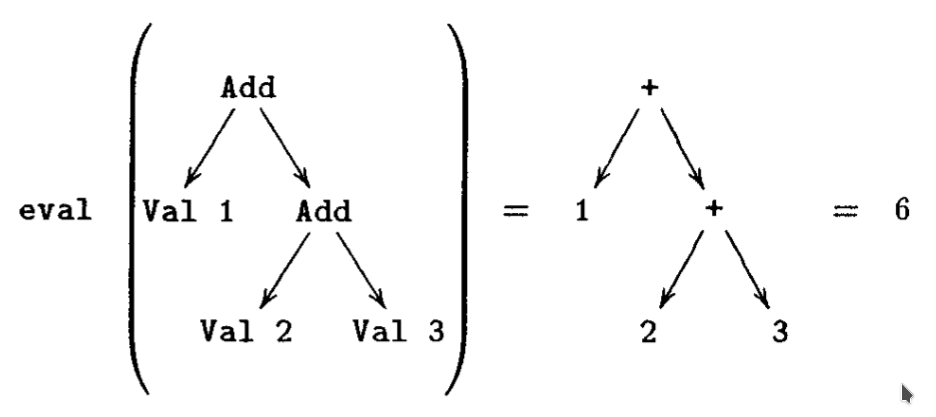
\includegraphics[width=0.6\textwidth]{figs/eval-prog}
    \caption{Денотационная семантика определяет смысл синтаксических конструкций через операции над доменом~\cite{hutton1998fold}.}
    \label{fig:eval-prog}
\end{figure}

Другим популярным стилем описания семантики является \vocab{операционная семантика}, которая представляет смысл программы в виде последовательности шагов вычислений.
Это может быть как последовательное переписывание самого выражения, так и переписывание состояния некоторой абстрактной машины.
Операционная семантика, в свою очередь, задаётся как развёртка (или анаморфизм~\ref{subsubsec:recursion-schemas}) последовательности шагов вычисления из программы.
Тут отчётливо видна некоторая двойственность между денотационной и операционной семантиками~\cite{hutton1998fold}.

\subsubsection{Встроенные доменно-специфичные языки (eDSL)} \label{subsubsec:edsl}

Под \vocab{доменно-специфичными языками (domain specific languages, DSL)}\footnote{\url{https://en.wikipedia.org/wiki/Domain-specific_language}} часто понимают специализированные языки для конкретных предметных областей, например, запросов к БД или форматирования документов.
Как правило, такие языки не являются полными по Тьюрингу.

В этом курсе, однако, мы будем считать доменно-специфичным языком любую доменно-специфичную специализацию языка общего назначения\footnote{\url{https://en.wikipedia.org/wiki/Language-oriented_programming}, на русскоязычную страницу тоже следует заглянуть.}.
Это следует из того соображения, что код должен читаться как грамотная проза с уместным словоупотреблением, предоставляющая читателю только необходимое количество подробностей, скрывая несущественное за умолчаниями и терминологией.

\vocab{Самостоятельные доменно-специфичные языки (standalone domain specific languages)} --- языки, имеющие свой собственный конкретный синтаксис, а так же инструменты программирования (IDE, исполняющая среда\ldots).
Примеры: SQL, AWK, Antlr\ldots\footnote{Есть отличная прикладная книга~\cite{nystrom2021crafting}, рассказывающая о построении интерпретаторов и простых виртуальных машин.
В то же время она покрывает сознание полноценного языка во всех его аспектах, от синтаксического анализа до управления памятью.}

\vocab{Встроенные доменно-специфичные языки (embedded domain specific languages, eDSL)} --- языки, пользующиеся поддержкой инфраструктуры других языков.
Обычно реализуются как библиотеки для программ на уже существующем языке общего назначения.
Не имеют полностью собственного конкретного синтаксиса.
Примеры: ORM, функции обработки строк, библиотека парсер-комбинаторов\ldots

\vocab{Deep eDSL} --- термы на таком языке строят дерево абстрактного синтаксиса для дальнейшей интерпретации:
\begin{minted}{haskell}
    f :: Int -> Int
    f = eval $ Const 1 `Plus` Input
\end{minted}

Интерпретаторы, которые принимают деревья на вход и интерпретируют их в семантический домен, называют \vocab{инициальными}\footnote{Тип синтаксиса заданный с помощью \mintinline{haskell}{data} является инициальным объектом категории интерпретаций.}, мы их также будем называть ``классическими''.
С них мы и будем начинать.
Классические интерпретаторы полезны, например, как для реализации ``последнего языка''~--- интерфейса программы во внешний мир, и как фундамент для наших дальнейших построений.

%Например, можно построить встроенный язык для работы с изменяемым состоянием.
%Теперь можем писать императивно в Haskell без единой монады!
%\begin{minted}{haskell}
%    fac :: Int -> Int
%    fac = eval $
%
%\end{minted}

Однако, можно заметить, что промежуточное дерево, которое получается, нас, как правило, не интересует.
Нам важно только получить элемент домена, которым мы уже умеем пользоваться непосредственно.
\vocab{Shallow eDSL} минуют стадию построения дерева и сразу строят значение в семантическом домене.
Такие интерпретаторы мы будем называть \vocab{финальными}\footnote{Такой способ задания интерпретаторов называют финальным по историческим причинам. Казалось, что соответствующие программы соответствуют терминальному (финальному) объекту категории интерпретаций. Однако, как оказалось, с категорной точки зрения, это тоже инициальный объект.}.
\begin{minted}{haskell}
    cnst :: Int -> (Int -> Int)
    cnst x _ = x

    input :: Int -> Int
    input env = env

    plus :: (Int -> Int) -> (Int -> Int) -> (Int -> Int)
    plus l r env = l env + r env

    f :: Int -> Int
    f = cnst 1 `plus` input
\end{minted}

Интерпретаторы часто называют \vocab{наблюдателями (observers)}, которые анализируют термы и дают им некоторый смысл~\cite{gibbons2013functional}.
Можно заметить, что для deep eDSL можно написать сколь угодно много различных наблюдателей.
Однако в случае shallow embedding наблюдатели всегда \texttt{id}.
Мы будем обсуждать возможные решения этой проблемы далее в разделе~\ref{subsubsec:shallow-embedding}.

Обсуждение терминологии и сравнение подходов к построению DSL можно найти в~\cite{gibbons2013functional}.
Краткое описание терминов --- в конспекте курса Language Engineering~\cite{languageEngineering}.

Введём ещё одно важное понятие.
\vocab{Meta-circular интерпретатор}\footnote{\url{https://en.wikipedia.org/wiki/Meta-circular_evaluator}}~--- это интерпретатор, определяющий конструкции определяемого языка через конструкции мета-языка~\cite{reynolds1972definitional}.
Например:
\begin{minted}{haskell}
    interpret term = case term of
      App f t -> (interpret f) (interpret t)
      If c t e -> if interpret c then interpret t else interpret e
      ...
\end{minted}

Свойства мета-языка в таком случае во многом определяют свойства объектного~\cite{reynolds1972definitional,reynolds1998definitional}.
Мы будем в этом курсе стремиться как можно более переиспользовать возможности мета-языка.

\begin{task}
    Предположите, какие свойства наследует определяемый язык из примера выше.
\end{task}

\subsubsection{Пример: библиотека Accelerate}

Интересным примером встроенного языка, находящегося где-то между deep и shallow является библиотека Accelerate\footnote{\url{https://hackage.haskell.org/package/accelerate}}~\cite[глава 6]{marlow2011parallel}.
Она позволяет на Haskell описать вычисления, которые будут исполняться на GPU\footnote{Другой подход: \href{https://youtu.be/6c0DB2kwF_Q?si=-nB7AkCsDWB_Q-hy}{Java code reflection}, чтобы в рантайме извлекать модель кода. Однако, такой подход не предоставляет статически гарантий программисту и требует глубогоко внедрения в мета-язык.}.

Чтобы исполнить что-то на GPU, нужно породить и скомпилировать код на Cuda.
Таким образом, Accelerate должен быть deep embedding, чтобы иметь дерево вычисления, чтобы его транслировать в Cuda наиболее эффективным образом.

В то же время описывать численные вычисления как дерево крайне неудобно.
Неплохо было бы иметь привычные операторы и функции высших порядков для работы с массивами на GPU\@.
Поэтому Accelerate предоставляет на самом деле shallow интерфейс для построения деревьев.
Так, для деревьев выражений определена реализация численных классов типов, например, \mintinline{haskell}|Num|, где операции просто достраивают дерево:
\begin{minted}{haskell}
    example :: Acc (Vector Int) -> Acc (Vector Int) -> Acc (Vector Int)
    example xs ys = A.zipWith (+) xs ys
\end{minted}

\subsection{Типы значений}

Рассмотрим, какие есть способы реализации языков, значения в которых могут иметь различные типы.

\subsubsection{Untyped tagless interpreters}

Для начала рассмотрим некоторый тривиальный нетипизироватный язык.
Под нетипизированностью понимаем отсутствие проверки типов как до исполнения программы, так и во время.
Абстрактный синтаксис этого языка зададим следующим образом:
\begin{minted}{haskell}
    data Expr = Const Int | IsZero Expr | If Expr Expr Expr
\end{minted}

Значения, возникающие во время исполнения программ на этом языке будем представлять значениями типов \mintinline{haskell}|Bool| и \mintinline{haskell}|Int| языка Haskell.
Соответственно, семантическим доменом программы на этом языке является либо \mintinline{haskell}|Bool|, либо \mintinline{haskell}|Int|, в зависимости от самой программы.
\begin{minted}{haskell}
    evalUnsafe :: Expr -> forall res . res
    evalUnsafe = \case
      Const val -> unsafeCoerce val
      IsZero cond -> unsafeCoerce $ evalUnsafe @Int cond == 0
      If c t e -> if evalUnsafe c then evalUnsafe t else evalUnsafe e
\end{minted}

Здесь \texttt{unsafeCoerce} используется, чтобы обмануть статическую систему типов Haskell и просто исполнять программы на нашем нетипизированном языке.
Мы имеем право так делать, поскольку \mintinline{haskell}{Int} и \mintinline{haskell}{Bool} в Haskell имеют одинаковый размер.
Неверное написание программы на этом языке или выбор неправильного домена интерпретации приводят к падению.

\subsubsection{Typed tagged interpreters}

Чтобы добиться некоторой безопасности исполнения, будем приписывать значениям теги, которые будут доступны во время исполнения.
Заведём следующий алгебраический тип:
\begin{minted}{haskell}
    data RtValue = RtBool Bool | RtInt Int
\end{minted}

Теперь семантическим доменов у нас будет тип \mintinline{haskell}|RtValue|, а интерпретатор сможет проверять типы во время исполнения:
\begin{minted}{haskell}
    evalRt :: Expr -> RtValue
    evalRt (IsZero expr) = case evalRt expr of
      RtBool value -> error "Type error"
      RtInt value -> RtBool (value == 0)
    -- ...
\end{minted}

Ситуация с безопасностью программы определённо стала лучше, однако проверка типов во время исполнения~--- это уже поздно: требует дополнительных расходов производительности и удорожает тестирование.

Этот подход часто называют \vocab{динамической типизацей}, когда мы атрибутируем значения некоторой типовой информацией для использования во время исполнения (см.\ также\ \ref{subsubsec:type-reflection}).

\subsubsection{Typed tagless interpreters} \label{subsubsec:typed-tagless-initial}

Опишем систему типов нашего маленького языка.
%! suppress = EscapeAmpersand
\begin{equation*}{}
    \infer[Const]{Const~n : int}{n : Int}
    \quad
    \infer[IsZero]{IsZero~n : bool}{n : int}
    \quad
    \infer[If]{If~c~t~e : \tau}{c : bool & t : \tau & e : \tau}
\end{equation*}
Можем в качестве типовых тегов переиспользовать типы Haskell: \[int \rightsquigarrow Int, bool \rightsquigarrow Bool\]

Заметим, что с помощью обобщённого алгебраического типа данных \mintinline{haskell}|Expr ty| (\ref{subsubsec:gadts}), мы как раз закодировали эти правила вывода.
Иначе говоря, мы получили статически типизированный язык программирования, переиспользовав систему типов Haskell.
\begin{minted}{haskell}
    data Expr ty where
      Const :: Int -> Expr Int
      IsZero :: Expr Int -> Expr Bool
      If :: forall ty . Expr Bool -> Expr ty -> Expr ty -> Expr ty

    eval :: Expr ty -> ty
    eval = \case
      Const n -> n
      IsZero e -> eval e == 0
      If c t e -> if eval c then eval t else eval e
\end{minted}

Благодаря статической типизации, мы можем отказаться от тегирования значений во время интерпретации без потери безопасности.

\subsection{Связывания и функции первого класса} \label{subsec:first-class-functions}

В этом параграфе мы рассмотрим техники и понятия, относящиеся к реализации функций первого класса и связываний в общем.
Поскольку эта функциональность уже, как правило, реализована в мета-языке, мы будем стремиться её максимально переиспользовать.

\mintinline{haskell}|let|-связывания можно представить через функции первого класса следующим образом:
\[
    \term{let} \ap x \termdef N \ap \term{in} \ap M \equiv (\lambda x\ldotp M) \ap N
\]

Напомним, что от функций первого класса можно избавиться с помощью дефункционализации, рассмотренной ранее~\ref{subsubsec:defunctionalization}.

\subsubsection{Связывание имён} \label{subsubsec:name-bindings}

Существует несколько способов задания семантики идентификаторам.

\vocab{Динамическое связывание (dynamic scoping)} --- значение свободных переменных функции зависит от области видимости в месте вызова.
То есть разрешение имени происходит в момент обращения к переменной.
Например, следующий код напечатает \texttt{42}:
\begin{minted}{scala}
    val f = () => {
        val x = 4
        () => x + 1
    }
    val x = 41
    println(f())
\end{minted}

Этот подход проще в реализации и использовался в ранних версиях Lisp'ов, например.
Однако в таком случае функции не являются надежным барьером абстракции, по-хорошему все свободные переменные должны являться частью сигнатуры (вернёмся в этому в главе про системы эффектов~\ref{sec:effect-systems}).

\vocab{Лексическое/статическое связывание (lexical/static scoping)} --- переменные связываются со значениями в момент объявления функции, в момент вызова результат зависит только от параметров (по модулю изменяемого состояния\footnote{Например, в Kotlin в лямбды можно захватывать изменяемые переменные. Изменения снаружи наблюдаемы внутри лямбды, и наоборот. Иногда это может быть очень удобно, однако нередко приводит к очень неочевидному поведению.}).
Слово ``лексический'' часто употребляется в языках, когда мы что-то можем понять из исходного кода без запуска программы.
Так, код из примера выше напечатает 5.

Далее в этом разделе мы будем говорить о различных способах реализации функций первого класса со статическим связыванием переменных, которых, на самом деле, великое множество\footnote{\url{https://jesper.cx/posts/1001-syntax-representations.html}}.

\subsubsection{Подстановки} \label{subsubsec:substitutions}

Как можно заметить, в классическом лямбда-исчислении подстановки от бета-редукции (вспоминали в разделе~\ref{subsec:terms-reduction}) обеспечивают статическое связывание.
Действительно, аргумент немедленно подставляется во все вхождения переменной, соответственно она не остаётся свободной, а просто исчезает.
\[
    (\lambda x\ldotp (\lambda x\ldotp \lambda y\ldotp x + y) \ap 4) \ap 41 \rightsquigarrow (\lambda x\ldotp (\lambda y\ldotp 4 + y)) \ap 41
\]

Такой подход не является самым эффективным, потому что на каждую аппликацию требуется переписывать код функции целиком (!).
В то же время его довольно просто реализовать для некоторых представлений лямбда-термов.
Рассмотрим пример такого представления --- \vocab{locally nameless}~\cite{chargueraud2012locally}.

\begin{minted}{haskell}
    data Term var
      = Var var
      | App (Term var) (Term var)
      | Lam (Term (Maybe var))
\end{minted}

В этом представлении можно выбирать любой тип для именования свободных переменных:
\begin{minted}{haskell}
    example :: Term String
    example = Var "x" `App` Var "y" -- x y
\end{minted}
Добавление каждой связанной переменной добавляет типу переменных нового обитателя \mintinline{haskell}|Nothing| для обращения к ближайшей связанной переменной:
\begin{minted}{haskell}
    -- ?$\lambda x\ldotp x \ap y$?
    example1 = Lam $ Nothing `App` Just "y"
    -- ?$\lambda x \ap y\ldotp x \ap y \ap z$?
    example2 = Lam $ Lam $ Just Nothing `App` Nothing `App` Just (Just "z")
\end{minted}

Монадический bind является реализацией подстановки для таких термов:
\begin{minted}{haskell}
    instance Monad Term where
      (>>=) :: Term var -> (var -> Term var') -> Term var'
      Var var >>= subst = subst var
      App l r >>= subst = App (l >>= subst) (r >>= subst)
      Lam t >>= subst = Lam $ t >>= \case
        Nothing  -> Var Nothing
        Just var -> Just <$> subst var
\end{minted}

\begin{task}
    Подумайте, зачем нужен \texttt{fmap Just} в последней строчке.
\end{task}

Соответственно, call-by-name интерпретатор такого лямбда-исчисления будет выглядеть следующим образом:\footnote{Поскольку мы рассматриваем классическое $\lambda$-исчисление, в качестве результирующего значения мы получаем тоже терм, но в нормальной форме.}

\begin{minted}{haskell}
    eval :: Term var -> Term var
    eval = \case
      Var var -> Var var
      App f arg -> case eval f of
        Lam body -> eval $ body >>= maybe arg Var
        t -> App t (eval arg)
      Lam t -> Lam (eval t)
\end{minted}

\subsubsection{Окружение}

Можно делать подстановку значений переменных лениво, распространяя окружение, которое ставит в соответствие свободным переменным термы.
Лучше, в целом, пока не стало, но мы получили композиционную семантику из некомпозиционной путём эксплицирования контекстных зависимостей (подробнее далее~\ref{subsubsec:recover-compositionality}).

\begin{minted}{haskell}
    data Term1 = Var1 String | App1 Term1 Term1 | Lam1 String Term1
    type Env = Map String Term1

    eval1 :: Term1 -> Env -> Term1
    eval1 term env = case term of
      Var1 name -> Map.findWithDefault (Var1 name) name env
      App1 f arg -> case eval1 f env of
        Lam1 name body -> eval1 body (Map.insert name arg env)
        t -> App1 t (eval1 arg env)
      Lam1 name body ->
        let env' = Map.delete name env in
        Lam1 name (eval1 body env')
\end{minted}

\begin{task}
    Объясните, зачем окружение модифицируется на строчке~10?
\end{task}

Если ветка \mintinline{haskell}|Lam1| не будет рекурсивно обходить подтерм и подставлять значения переменных, информация о значениях свободных переменных в нём потеряется и мы получим динамическое связывание вместо статического.
Чтобы восстановить статическое связывание, ветка \mintinline{haskell}|Lam1| интерпретатора должна конструировать замыкание, включающее текущее окружение (см.\ далее~\ref{subsubsec:closures}).

\subsubsection{Замыкания} \label{subsubsec:closures}

Чтобы не делать энергично подстановку в тела функций и сохранить при этом статическое связывание, добавим ещё одну конструкцию, \vocab{замыкание (closure)}\footnote{\url{https://en.wikipedia.org/wiki/Closure_(computer_programming)}}\footnote{Термин closure был предложен Piter Landin, вместе с кучей других вещей.}~\cite[глава 11]{nystrom2021crafting}.
Оно будет хранить контекст, в котором должен исполняться соответствующий терм.

\begin{minted}{haskell}
    data Term1 = Var1 String | App1 Term1 Term1 | Lam1 String Term1
               | Closure Env String Term1 -- только для вычислений
    type Env = Map String Term1

    eval1 :: Term1 -> Env -> Term1
    eval1 term env = case term of
      Var1 name -> Map.findWithDefault (Var1 name) name env
      App1 f arg -> case eval1 f env of
        Closure env' body -> eval1 body (Map.insert name arg $ env <> env')
        t -> App1 t (eval1 arg env)
      Lam1 name body -> Closure env name body
\end{minted}

Замыкания обычно и используют в промышленных языках как представление времени исполнения функций высших порядков.
Во время компиляции сначала производят \vocab{closure conversion}~--- функции высших порядков представляют как пару из окружения и указателя на функцию, принимающую окружение дополнительным аргументом.
Теперь, когда функция не содержит свободных переменных, делают \vocab{lambda lifting}\footnote{\url{https://en.wikipedia.org/wiki/Lambda_lifting}}~--- поднимают её на верхний уровень.
Подробные примеры можно посмотреть в гарвардских слайдах~\cite{closures-slides}.

\subsubsection{Типизированный контекст} \label{subsubsec:typed-env}

Рассмотрим кодирование, описанное, например, в~\cite{kiselyov2012typed}.

Для начала научимся с помощью системы типов Haskell проверять валидность обращения к окружению.
Представим окружение как список типов, закодированный с помощью вложенных пар:
\begin{minted}{haskell}
    (4, (4.0, "hello")) :: (Int, (Double, String))
\end{minted}

Обращение к окружению будем кодировать числом в унарной записи.
Тип числа (типизированной ссылки внутрь контекста) пусть задаёт множество окружений \texttt{env}, из которых на данной позиции можно извлечь тип \texttt{ty}.
\begin{minted}{haskell}
    data Ref env ty where
      Here :: Ref (ty, env) ty
      There :: Ref env ty -> Ref (ty', env) ty
\end{minted}
Например, тип числа 1 утверждает, что с его помощью можно извлечь значение типа \texttt{ty} из контекста, в котором значение соответствующего типа находится на первой позиции (нумерация с нуля):
\begin{minted}{haskell}
    There Here :: Ref (ty', (ty, env)) ty
\end{minted}

Теперь мы можем закодировать типизированное безопасное обращение к контексту:
\begin{minted}{haskell}
    envLookup :: env -> Ref env ty -> ty
    envLookup env ref = case (ref, env) of
      (Here, (x, _)) -> x
      (There ref', (_, env')) -> envLookup env' ref'
\end{minted}

\begin{task}
    Можно ли разобрать пару сразу на строчке 2?
    Поясните.
\end{task}

\subsubsection{Meta-circular интерпретация} \label{subsubsec:meta-circular-initial}

Крайне не хотелось бы для eDSL самостоятельно реализовывать связывания и функции первого класса.
Построим meta-circular интерпретатор (см.~\ref{subsubsec:edsl}), который будет переиспользовать функции первого класса мета-языка для реализации их в определяемом языке.

Термы теперь будут не только аннотированы результирующими типами, но и типами необходимых для интерпретации окружений, рассмотренных ранее~\ref{subsubsec:typed-env}.
Абстрагированному терму доступно большее окружение.

\begin{minted}{haskell}
    data Term2 env ty where
      Var2 :: Ref env ty -> Term2 env ty
      App2 :: Term2 env (arg -> res) -> Term2 env arg -> Term2 env res
      Lam2 :: Term2 (arg, env) res -> Term2 env (arg -> res)
\end{minted}

Теперь абстракцию можем проинтерпретировать в функцию Haskell, а аппликацию --- в аппликацию:
\begin{minted}{haskell}
    eval2 :: Term2 env ty -> env -> ty
    eval2 term env = case term of
      Var2 ref -> env `envLookup` ref
      App2 f arg -> (eval2 f env) (eval2 arg env)
      Lam2 t -> \arg -> eval2 t (arg, env)
\end{minted}

\begin{task}
    Как так получилось, что в последней строчке нужно принять ещё один аргумент?
\end{task}

\begin{task}
    Это call-by-value интерпретатор или call-by-name?
    От чего это зависит?
\end{task}

\begin{task}
    Подумайте, какое решение должно быть более производительно, это или предыдущее?
\end{task}

Обратите внимание, что теперь функции определяемого языка во время исполнения --- это просто функции мета-языка.
А значит, в программах на определяемом языке мы \point{можем полностью переиспользовать мета-язык}!
Добавим для этого конструкцию, позволяющую сохранить произвольное значение мета-языка в дереве:
\begin{minted}{haskell}
    data Term2 env ty where
      Val2 :: ty -> Term2 env ty
      -- ...

    eval2 :: Term2 env ty -> env -> ty
    eval2 term env = case term of
      Val2 x -> x
      -- ...

    example :: Term2 env (Int -> Int)
    example = Lam (Val2 (+) `App2` Val2 1 `App2` Var2 Here)
\end{minted}

\subsubsection{Синтаксис высшего порядка} \label{subsubsec:h-syntax}

Ещё чем мы ещё занимаемся вручную --- определяем связыватели (да ещё и в унарной записи).
Хотим переиспользовать их из мета-языка.
Для это мы будем прямо в дереве синтаксиса хранить функции мета-языка~--- использовать \vocab{синтаксис высшего порядка (higher order abstract syntax)}\footnote{\url{https://en.wikipedia.org/wiki/Higher-order_abstract_syntax}}\footnote{\href{https://cstheory.stackexchange.com/questions/20071/what-is-higher-order-in-higher-order-abstract-syntax}{What is higher-order in higher-order abstract syntax?}}~\cite{pfenning1988higher}:
\begin{minted}{haskell}
    data Term3 ty where
      Val3 :: ty -> Term3 ty
      Plus :: Term3 Int -> Term3 Int -> Term3 Int
      App3 :: Term3 (arg -> res) -> Term3 arg -> Term3 res
      Lam3 :: (Term3 arg -> Term3 res) -> Term3 (arg -> res)

    example3 :: Term3 Int
    example3 = (Lam3 \x -> x `Plus` Val3 41) `App3` Val3 1
\end{minted}

Интерпретация очень простая и абсолютно meta-circular:
\begin{minted}{haskell}
    eval3 :: Term3 ty -> ty
    eval3 term = case term of
      Val3 x -> x
      Plus l r -> eval3 l + eval3 r
      App3 f arg -> (eval3 f) (eval3 arg)
      Lam3 f -> \arg -> eval3 (f (Val3 arg))
\end{minted}

\begin{task}
    Можно ли было объявить \mintinline{haskell}|Lam3| следующим образом?
    \begin{minted}{haskell}
        Lam3 :: (arg -> Term3 res) -> Term3 (arg -> res)
    \end{minted}
\end{task}

\subsubsection{Сериализация функций}

В этом разделе мы говорили о возможных реализациях функций первого класса, то есть функций, которые можно использовать так же гибко, как и данные.
Возникает закономерный вопрос: можем ли мы сериализовать функцию первого класса и послать исполняться на другую машину?

Функция состоит из кода и захваченных свободных переменных в случае статического связывания.
Соответственно, если код представлен в сериализуемом виде (например, позиционно-независимый байт-код), то его в принципе можно переслать по сети и исполнить на другом инстансе виртуальной машины.
Так, например, делает Erlang.
Однако, такой подход неэффективный, так как байт-код нужно интерпретировать или предварительно компилировать.
Таким образом, Erlang жертвует скоростью исполнения ради горизонтальной масштабируемости.

Если мы гарантируем, что на различных узлах кластера исполняется один и тот же код, как обычно и бывает на практике, можно добиться более эффективной реализации.
Например, используя дефункционализацию~(см.~\ref{subsubsec:defunctionalization}), мы можем сериализовать только объекты алгебраического типа, кодирующие функции.
Поскольку на другом узле кластера исполняется такой же код, мы там можем десериализовать объект и исполнить его с помощью \texttt{apply}.
Однако этот подход не очень поддерживает модульность (сложно один алгебраический тип разбить на много), а так же \texttt{apply} каждый раз производит декодирование перед исполнением кода (чем, в прочем, можно пренебречь, учитывая работу с сетью).

Подход, реализованный в Haskell\footnote{\url{https://blog.ocharles.org.uk/blog/guest-posts/2014-12-23-static-pointers.html}}\footnote{\url{https://hackage.haskell.org/package/distributed-closure}} позволяет наделить каждую функцию без свободных переменных некоторым статически известным адресом, одинаковым для всех инстансов приложения.
Далее можно сконструировать сериализуемое замыкание путём последовательности частичных применений:
\begin{minted}{haskell}
    data Closure a where
      StaticPtr :: StaticPtr b -> Closure b
      Encoded :: ByteString -> Closure ByteString
      Ap :: Closure (b -> c) -> Closure b -> Closure c

    main = send "some-node" $
      closure (static factorial) `closureAp` closurePure 10
\end{minted}

Подробнее можно прочитать в основополагающей статье про облачный Haskell~\cite{epstein2011towards}.
С практической точки зрения --- в книжке~\cite[глава 16]{marlow2011parallel}.

\begin{task}
    Нужно ли явно добавлять в замыкание свободную переменную \texttt{(*)} (оператор умножения) в реализации факториала?
\end{task}

\subsection{Tagless final интерпретаторы} \label{subsec:tagless-final}

Как мы убедились ранее (\ref{subsec:interpreters-everywhere}), программирование состоит из написания новых и новых интерпретаторов поверх друг друга.
Интерпретаторы задают семантику новых языков (\ref{subsec:semantics}).
В классическом виде язык задаётся как множество деревьев, а интерпретатор отправляет деревья в объект мета-языка.
Если язык встроенный, то такой подход называют deep embedding (см.~\ref{subsubsec:edsl}), а соответствующий интерпретатор инициальным.
\[
    \sembr{\bullet} : L \to D
\]

Можно заметить, что в конечном итоге мы используем только элемент домена, в который интерпретатор отображает программу.
Сама программа же представляет собой лишь удобную синтаксическую запись элемента домена и является промежуточным шагом, а не самоцелью.
В то же время доменом в случае встроенных языков, заданных интерпретаторами, являются объекты мета-языка.
Можем ли мы миновать стадию интерпретации собственного синтаксиса и сразу строить объект домена в синтаксисе мета-языка?
Да, такое встраивание называется shallow embedding (\ref{subsubsec:edsl}), о нём эта глава.

\subsubsection{Разные интерпретации для shallow embedding} \label{subsubsec:shallow-embedding}

Как мы узнали ранее (\ref{subsec:all-folds}), любую структуру данных можно представить свёрткой.
И, более того, в итоге можно обойтись без единого конструктора данных (как в списке Чёрча, например): алгебра представляется набором функций, каждая из которых отвечает за сворачивание определённого конструктора.
\begin{minted}{haskell}
    Fix f ?$\iso$? forall a . (f a -> a) -> a
    List e ?$\iso$? forall a . (e -> a -> a) -> a -> a
\end{minted}

Таким образом, вместо того, чтобы конструировать дерево языка, а затем его интерпретировать (сворачивать), мы можем сразу сконструировать терм типа \mintinline{haskell}{?$\forall$?a . (f a -> a) -> a}.
Предоставив ему тип домена \texttt{a} и алгебру \texttt{f a -> a} (либо в виде пачки функций), мы немедленно получим элемент нужного домена.
Чтобы задать другую интерпретацию, нужно передать другой тип домена и алгебру:
\begin{minted}{haskell}
    example :: (Int -> a) -> (a -> a -> a) -> a
    example cnst plus = cnst 1 `plus` cnst 41

    ghci> example show (\l r -> l ++ " + " ++ r)
    "1 + 41"
\end{minted}

Если зафиксировать интерпретацию, то функции-аргументы можно реализовать статически и просто ссылаться на них в терме.
Таким образом, про объявление функций можно думать как про расширение некоторого встроенного предметного языка.
Общие рассуждения про shallow embeddings, свёртки и библиотеки можно почитать в~\cite{gibbons2013functional, gibbons2014folding}.
Сравните:
\begin{figure}[h]
    \centering
    \begin{tabular}{|p{0.45\linewidth}|p{0.45\linewidth}|}
        \hline
        Deep                                                                                                                                 & Shallow                                                                              \\
        \hline
        Синтаксис языка задаётся набором допустимых нод дерева                                                                               & Декларация функции задаёт новую ноду дерева: вызов этой функции                      \\
        \hline
        Интерпретатор при виде каждой ноды выполняет соответствующий код на мета-языке (ветку паттерн-матчинга) после вычисления поддеревьев & Интерпретатор при виде вызова выполняет код тела функции после вычисления аргументов \\
        \hline
    \end{tabular}
\end{figure}

\subsubsection{Дойти до конца}

Вернёмся к некаррированной версии свёрток: теперь это тип, принимающий кортеж функций.
А кортеж функций можно заменить на класс типов.
Тогда декларация класса будет задавать синтаксис встроенного языка, а инстансы для доменов~--- реализацию.
Этот подход называется \vocab{tagless final encoding}\footnote{\url{https://okmij.org/ftp/tagless-final/}} и фактически это кодирование данных по Чёрчу с классами типов и набором трюков~\cite{carette2007finally, kiselyov2012typed}.

Снова рассмотрим язык со сложением:
\begin{minted}{haskell}
    data Expr = Const Int | Plus Expr Expr

    eval :: Expr -> Int
    eval = \case Const x -> x; Plus l r -> eval l + eval r
\end{minted}
Или через катаморфизм:
\begin{minted}{haskell}
    data ExprF rec = Const Int | Plus rec rec

    eval :: Fix ExprF -> Int
    eval = cata \case Const x -> x; Plus l r -> l + r
\end{minted}
Соответствующее tagless final кодирование будет выглядеть следующим образом:
\begin{minted}{haskell}
    class Expr domain where
      cnst :: Int -> domain
      plus :: domain -> domain -> domain

    instance Expr Int where
      cnst x = x
      plus l r = l + r
\end{minted}

Теперь мы можем сконструировать обычный терм Haskell, задать домен, и машинерия классов типов подставит нужную алгебру самостоятельно:
\begin{minted}{haskell}
    example :: forall domain . Expr domain => domain
    example = cnst 1 `plus` cnst 41

    ghci> example :: Int
    42
\end{minted}

Чтобы добавить ещё интерпретацию, реализуем инстанс для другого домена:
\begin{minted}{haskell}
    instance Expr String where
      cnst x = show x
      plus l r = l <> " + " <> r

    ghci> example :: String
    "1 + 41"
\end{minted}

\subsubsection{Восстановление композиционности семантики} \label{subsubsec:recover-compositionality}

\vocab{Семантика} называется \vocab{композиционной}, если семантика конструкций зависит только от семантик подконструкций (см.~\ref{subsec:semantics}).
Иначе говоря, она может быть задана катаморфизмом и, соответственно, инстансом класса типов в tagless final.
То есть, чтобы уметь для любой семантики построить tagless final реализацию, нужно уметь универсальным образом превращать некомпозиционные семантики в композиционные.

Всякие преобразования кода, как правило, не композиционные.
Для примера рассмотрим протаскивание унарных отрицаний:
\begin{minted}{haskell}
    data Expr1 = Lit Int | Add Expr1 Expr1 | Neg Expr1

    transform1 :: Expr1 -> Expr1
    transform1 = \case
      Lit x -> Lit x
      Add l r -> Add (transform1 l) (transform1 r)
      Neg (Lit x) -> Lit (-x)                                        -- проблема
      Neg (Neg e) -> transform1 e                                    -- проблема
      Neg (Add l r) -> Add (transform1 (Neg l)) (transform1 (Neg r)) -- проблема
\end{minted}
Чтобы восстановить композиционность семантики, нужно экплицировать контекстные зависимости с помощью стрелочного домена домена~\cite{kiselyov2012typed}:
\begin{minted}{haskell}
    data Ctx = CtxPos | CtxNeg
    flipCtx = \case CtxPos -> CtxNeg; CtxNeg -> CtxPos

    transform1' :: Expr1 -> (Ctx -> Expr1)
    transform1' expr = case expr of
      Lit x -> \case CtxNeg -> List (-x); CtxPos -> Lit x
      Neg e -> \ctx -> transform1' e (flipCtx ctx)
      Add l r -> \ctx -> Add (transform1' l ctx) (transform1' r ctx)
\end{minted}
Отсюда можно получить tagless final версию:
\begin{minted}{haskell}
    class Expr2 d where
      lit :: Int -> d
      add :: d -> d -> d
      neg :: d -> d

    instance Expr2 d => Expr2 (Ctx -> d) where
      lit x = \case CtxNeg -> lit (-x); CtxPos -> lit x
      neg e = \ctx -> neg e (flipCtx ctx)
      add l r ctx = add (l ctx) (r ctx)
\end{minted}

\subsubsection{Typed tagless final interpreter}

Рассмотрим наш пример tagless initial encoding~\ref{subsubsec:typed-tagless-initial}:
\begin{minted}{haskell}
    data Expr ty where
      Const :: Int -> Expr Int
      IsZero :: Expr Int -> Expr Bool
      If :: forall ty . Expr Bool -> Expr ty -> Expr ty -> Expr ty

    eval :: Expr ty -> ty
    eval = \case
      Const x  -> x
      IsZero t -> eval == 0
      If c t e -> if eval c then eval t else eval e
\end{minted}
Чтобы получить final encoding, параметризуем домен результирующим типом выражения:
\begin{minted}{haskell}
    class Expr (domain :: Type -> Type) where
      cnst :: Int -> domain Int
      isZero :: domain Int -> domain Bool
      if' :: forall ty . domain Bool -> domain ty -> domain ty -> domain ty

    class Expr Identity where
      cnst x = Identity x
      isZero (Identity x) = Identity (x == 0)
      if' (Identity c) t e = if c then t else e
\end{minted}

\begin{task}
    Какой домен подойдёт для печати выражения?
\end{task}

%% todo перенести в домашку?
%Можно сделать константы полиморфными, но тогда разумно дать возможность реализациям наложить ограничения на их полиморфизм.
%Добьёмся этого с помощью ассоциированного семейства констреинтов:
%\begin{minted}{haskell}
%    class Expr domain where
%      type C domain ty :: Constraint
%      val :: C domain ty => ty -> domain ty
%      -- ...
%
%    instance Expr Identity where
%      type C Identity ty = ()
%      val x = Identity x
%      -- ...
%
%    instance Expr (Const String) Where
%      type C (Const String) ty = Show ty
%      val x = Const $ show x
%      -- ...
%
%    example :: forall domain . (C domain ty, Expr domain) => domain ty
%    example = val 42
%
%    ghci> example :: Const String Int
%\end{minted}
%
%\begin{minted}{haskell}
%     data Term3 ty where
%       Val3 :: ty -> Term3 ty
%       Plus :: Term3 Int -> Term3 Int -> Term3 Int
%       App3 :: Term3 (arg -> res) -> Term3 arg -> Term3 res
%       Lam3 :: (Term3 arg -> Term3 res) -> Term3 (arg -> res)
%
%     example3 :: Term3 Int
%     example3 = (Lam3 \x -> x `Plus` Val3 41) `App3` Val3 1
%
%     eval3 :: Term3 ty -> ty
%\end{minted}
%
%\begin{minted}{haskell}
%    class Term d where
%      type C d ty :: Constraint
%      val :: C d ty => ty -> d ty
%      plus :: d Int -> d Int -> d Int
%      app :: d (arg -> res) -> d arg -> d res
%      lam :: (d arg -> d res) -> d (arg -> res)
%
%    example :: (Term d, C d Int) => d Int
%    example = (lam \x -> x `plus` val 41) `app` val 1
%
%    instance Term Identity where
%      type C Identity ty = ()
%      val = Identity
%      plus = liftA2 (+)
%      app = liftA2 ($)
%      lam = coerce
%
%    instance Term (Const String) where
%      type C (Const String) ty = Show ty
%      val = Const . show
%      plus (Const l) (Const r) = Const $ "(" ++ l ++ " + " ++ r ++ ")"
%      app (Const f) (Const arg) = Const $ "(" ++ f ++ " " ++ arg ++ ")"
%      lam f = Const $ "(" ++ "\\x -> " ++ getConst (f (Const "x")) ++ ")"
%\end{minted}

\subsubsection{Встречаем старых друзей: \mintinline{haskell}{Applicative}, \mintinline{haskell}{Monad}}

Рассмотрим следующий язык в initial encoding с higher order abstract syntax (см.~\ref{subsubsec:meta-circular-initial}, ~\ref{subsubsec:h-syntax}).
Справа перепишем в tagless final, выбирая подходящие имена для кусков синтаксиса.

\begin{tabular}{p{8cm}p{8cm}}
    \begin{minted}[numberblanklines=true]{haskell}
        data Expr s ty where
          Val   :: ty -> Expr s ty
          App   :: Expr s (arg -> res)
                -> Expr s arg
                -> Expr s res


          LetIn :: Expr s ty
                -> (ty -> Expr s ty')
                -> Expr s ty'


          Get   :: Expr s s
          Put   :: s -> Expr s ()
    \end{minted}
    &
    \begin{minted}[numberblanklines=true]{haskell}
        class Applicative domain where
          pure  :: ty -> domain ty
          (<*>) :: domain (arg -> res)
                -> domain arg
                -> domain res

        class Monad domain where
          (>>=) :: domain ty
                -> (ty -> domain ty')
                -> domain ty'

        class MonadState s domain where
          get :: domain s
          put :: s -> domain ()
    \end{minted}
\end{tabular}
\vspace{1em}

Реализуем функцию, модифицирующую значение в нашем новом языке:

\begin{tabular}{p{8cm}p{8cm}}
    \begin{minted}[numberblanklines=true]{haskell}
        --
        modify :: (s -> s) -> Expr s s
        modify f =
          Get `LetIn` \x ->
          Put (f x) `LetIn` \() ->
          Val x
    \end{minted}
    &
    \begin{minted}[numberblanklines=true]{haskell}
        --                    s -> (s, s)
        modify :: (s -> s) -> State s s
        modify f =
          get >>= \x ->
          put (f x) >>= \() ->
          pure x
    \end{minted}
\end{tabular}
\vspace{1em}

И до боли знакомую интерпретацию:

\begin{tabular}{p{8cm}p{8cm}}
    \begin{minted}[numberblanklines=true]{haskell}
        eval :: Expr s ty -> s -> (s, ty)
        eval = \case


          Val x -> \s -> (s, x)
          App fs xs -> \s1 ->
            let (s2, f) = eval fs s1 in
            let (s3, x) = eval xs s2 in
            (s3, f x)


          LetIn comp k -> \s ->
            let (s', x) = eval comp s in
            eval (k x) s'


          Get -> \s -> (s, s)
          Put s -> \_ -> (s, ())
    \end{minted}
    &
    \begin{minted}[numberblanklines=true]{haskell}
        newtype State s a = State
          { runState :: s -> (s, a) }

        instance Applicative (State s) where
          pure x = State \s -> (s, x)
          fs <*> xs = State \s1 ->
            let (s2, f) = runState fs s1 in
            let (s3, x) = runState xs s2 in
            (s3, f x)

        instance Monad (State s) where
          comp >>= k = State \s ->
            let (s', x) = runState comp s in
            runState (k x) s'

        instance MonadState s (State s) where
          get = State \s -> (s, s)
          put s' = State \s -> (s', ())
    \end{minted}
\end{tabular}
\vspace{1em}

Таким образом, \point{аппликативные функторы --- meta-circular язык с аппликацией}, а \point{монадический bind --- это фактически let-in в higher-order синтаксисе}.

Изначально использовать теор-категорное понятие монады\footnote{\url{https://ncatlab.org/nlab/show/monad+(in+computer+science)}} в $\lambda$-исчислении было предложено в~\cite{moggi1988computational}, чтобы удобнее записывать денотационную семантику\footnote{Часто сопутствующее монадам понятие эффекта мы рассмотрим далее~\ref{sec:effect-handlers}.}.
Это оказалось настолько удобно в моменте, что их стали использовать повсеместно в функциональном программировании, чтобы расширять простые функциональные языки различными могущественными возможностями без изменения самих языков~\cite{wadler1990comprehending, wadler1992essence}.
Был сформулирован Moggi's principle:
\begin{center}
    <<Computations of type $\alpha$ correspond to values of type $f\ap\alpha$>>
\end{center}

Использовать аппликативные функторы предложили существенно позже, чтобы избежать именования промежуточных шагов вычислений, когда в этом нет необходимости~\cite{mcbride2008applicative}.
Таким образом, аппликативы дают встроенный язык выражений, а монады --- язык стейтментов.

\subsubsection{Bytecode vs threaded code} \label{subsubsec:threaded-code}

% todo https://en.wikipedia.org/wiki/Threaded_code


\subsection{Expression problem} \label{subsec:expression-problem}

\vocab{Expression problem}\footnote{\url{https://en.wikipedia.org/wiki/Expression_problem}} или \vocab{проблема выразительности} --- это некоторый критерий выразительности языка программирования, сформулированный Wadler'ом в 1998\footnote{\url{https://homepages.inf.ed.ac.uk/wadler/papers/expression/expression.txt}}.
Ставится вопрос: насколько легко расширять синтаксис встроенного языка и добавлять новые интерпретации?
Иначе говоря, насколько легко добавлять новые разновидности данных и методы обработки.

Под ``легкостью'' подразумевается локальность: нужно ли править различные куски кода для этого.
Например, если синтаксис языка задан обычным алгебраическим типом данных, то добавить новую интерпретацию ``легко''~--- просто добавить новую рекурсивную функцию, а добавить новую синтаксическую конструкцию~--- ``сложно''~--- нужно изменить все интерпретаторы:
\begin{minted}{haskell}
    data Expr
      = Const Int
      | Plus Expr Expr -- добавляем

    eval :: Expr -> Int
    eval = \case Const x -> x; Plus l r -> eval l + eval r

    show :: Expr -> String
    show = \case Const x -> show x; Plus l r -> show l ++ " + " ++ show r
\end{minted}

Если язык задан, например, с помощью наследования, то, наоборот, расширить синтаксис легко --- добавить новый класс, а добавить интерпретацию сложно --- добавить реализацию метода в каждом классе: % todo наследование куда-то сюда укладывается?
\begin{minted}{kotlin}
    interface Lang {
        fun eval(): Int
        fun show(): String
    }
    class Const(val x: Int) : Lang {
        override fun eval() = x
        override fun show() = x.toString()
    }
    class Plus(val l: Lang, val r: Lang) : Lang {
        override fun eval() = l.eval() + r.eval()
        override fun show() = "$l + $r"
    }
\end{minted}

Оказывается, существуют подходы, позволяющие добиться ``лёгкости'' по обоим измерениям.
Мы уделим им много внимания в этом курсе.

Действительно, как мы обсуждали ранее~\ref{subsec:interpreters-tower}, программы представляют собой серию интерпретаторов.
Для всё той же борьбы со сложностью, важно уметь описывать эти интерпретаторы модульно --- задавать части языков отдельно друг от друга, и собирать нужные языки по месту из готовых блоков.
Это помогает составлять программы из простых переиспользуемых компонент, каждая из которых имеет чёткую зону ответственности.

Expression problem возникала и решалась много раз: expression problem, stable denotations, extensible (modular) interpreters.
Прошло немало времени, пока не возникло понимание, что всё это об одном и том же\footnote{\url{https://okmij.org/ftp/Computation/having-effect.html}}.

% todo Independently Extensible Solutions to the Expression Problem
% todo Extensibility for the Masses: Practical Extensibility with Object Algebras

\subsubsection{Копроизведение функторов} \label{subsubsec:functor-coprod}

Воспользуемся представлением данных как неподвижной точки функтора (см.~\ref{subsubsec:functor-fixpoint}).
В качестве модельного языка возьмём язык выражений со сложением:
\begin{minted}{haskell}
    data Basic rec = Const Int | Plus rec rec

    algBasic :: Basic Int -> Int
    algBasic = \case Const x -> c; Plus l r -> l + r

    evalBasic :: Fix Basic -> Int
    evalBasic = cata algBasic
\end{minted}

Заметим, что сумма (копроизведение) функторов формы даёт функтор формы, алгебра для которого получается из алгебр компонент\footnote{Пользуемся расширением \href{https://ghc.gitlab.haskell.org/ghc/doc/users_guide/exts/type_operators.html}{TypeOperators}.}:
\begin{minted}{haskell}
    data (l :+: r) rec = L (l rec) | R (r rec)

    (\/) :: (l a -> a) -> (r a -> a) -> ((l :+: r) a -> a)
    phi \/ psi = \case L l -> phi l; R r -> psi r
\end{minted}

Расширим наш язык чтением числа из окружения.
Следуя рассмотренной ранее денотационной семантике~\ref{subsec:semantics}, выберем функцию \mintinline{haskell}{Int -> Int} в качестве домена:
\begin{minted}{haskell}
    data Basic rec = Const Int | Plus rec rec
    data Input rec = Input

    algBasic' :: Basic (Int -> Int) -> Int -> Int
    algBasic' = \case Const x -> const x; Plus l r -> const (l + r)

    algInput :: Input (Int -> Int) -> Int -> Int
    algInput = \case Input -> \env -> env
\end{minted}

Таким образом, мы добились возможности отдельно определять куски синтаксиса и семантики языка, и собирать нужный язык по месту.
Напишем программу на нашем языке с неявным иммутабельным состоянием:
\begin{minted}{haskell}
    f :: Int -> Int
    f = cata (algBasic' \/ algInput) $
      In (L (Plus (In (L (Const 1))) (In (R Input)))) -- 1 + input
\end{minted}

Однако заметим, что пока мы не решили проблему полностью, так как интерпретация новой конструкции \mintinline{haskell}{Input} потребовала более сложный домен и нам пришлось переписывать интерпретацию старой для него: из \mintinline{haskell}{algBasic} в \mintinline{haskell}{algBasic'}.
Теперь мы понимаем, почему stable denotations~--- это ещё одно название для expression problem~\ref{subsec:expression-problem}.
Далее мы дополним это решение до полноценного~\ref{sec:effect-handlers}.

Полученный терм на встроенном языке пока имеет несколько чудовищную запись, но далее мы рассмотрим, как сделать термы встроенных языков неотличимыми от обычного кода мета-языка.

\subsubsection{Произведение алгебр}

% todo

Ранее, мы пытались решить expression problem путём композирования функторов формы с помощью открытого копроизведения, а также композирования алгебр (см.~\ref{subsubsec:functor-coprod}).
Перейдя к финальной версии того же самого, композирование становится намного эффективнее и удобнее.
Вместо копроизведения функторов теперь имеем произведение алгебр, представляемое контекстом классов типов.

Чтобы определить ещё одну конструкцию, просто задаём новый класс с желаемыми интерпретациями:
\begin{minted}{haskell}
    class Input domain where
      input :: domain

    instance Input (Int -> Int) where
      input = \env -> env
\end{minted}

Теперь нужно снова не забыть реализовать предыдущие операции \mintinline{haskell}{Expr} для нового домена \mintinline{haskell}{Int -> Int} и можно не лету композировать языки:
\begin{minted}{haskell}
    example :: forall domain . (Expr domain, Input domain) => domain
    example = cnst 1 `plus` input

    ghci> (example :: Int -> Int) 41
    42
\end{minted}

% todo


    \clearpage


    \section{Классические интерпретаторы}

%    %! suppress = MissingLabel

Итак, мы определили, что интерпретаторы --- это основа основ, потому что главная задача программиста --- борьба со сложностью, а главный инструмент этой борьбы --- использование подходящих доменно-специфичных языков, позволяющих думать только о важном, абстрагируя несущественные детали.

В течение этого курса мы будем учиться писать интерпретаторы.
В этом разделе --- классические, которые принимают деревья на вход и интерпретируют их в семантический домен.
Такие интерпретаторы задают deep eDSL (\ref{subsec:edsl}).
Далее мы научимся миновать этап построения дерева определяемого языка, полностью переиспользовать и напрямую расширять мета-язык новыми конструкциями (раздел~\ref{sec:wonder-interpreters}).
Классические интерпретаторы полезны как для реализации ``последнего языка'' --- интерфейса программы во внешний мир, и как фундамент для наших дальнейших построений (см., например, далее~\ref{subsec:to-wonderland}, ~\ref{sec:datatype-generic}).
Также, со временем мы изучим разные подходы к конструированию священного Граалю этой науки~--- расширяемых интерпретаторов~\ref{sec:effect-handlers}.

``Классические'' интерпретаторы часто называют \vocab{инициальными интерпретаторами}.
Слово ``инициальный'' тут относится к тому, что мы имеем дело с инициальным объектом категории интерпретаций.
Всё что нам нужно понимать, --- что инициальные интерпретаторы работают с деревом программы, заданным классически с помощью \mintinline{haskell}|data| (да, деревья можно задавать и по-другому).

Есть отличная книга~\cite{nystrom2021crafting}, рассказывающая о построении классических интерпретаторов и простых виртуальных машин.
В то же время она покрывает сознание полноценного языка во всех его аспектах, от синтаксического анализа до управления памятью.

\subsection{Типы значений}

Рассмотрим, какие есть способы реализации языков, значения в которых могут иметь различные типы.

\subsubsection{Untyped tagless interpreters}

Для начала рассмотрим некоторый тривиальный нетипизироватный язык.
Под нетипизированностью понимаем отсутствие проверки типов как до исполнения программы, так и во время.
Абстрактный синтаксис этого языка зададим следующим образом:
\begin{minted}{haskell}
    data Expr = Const Int | IsZero Expr | If Expr Expr Expr
\end{minted}

Значения, возникающие во время исполнения программ на этом языке будем представлять значениями типов \mintinline{haskell}|Bool| и \mintinline{haskell}|Int| языка Haskell.
Соответственно, семантическим доменом программы на этом языке является либо \mintinline{haskell}|Bool|, либо \mintinline{haskell}|Int|, в зависимости от самой программы.
\begin{minted}{haskell}
    evalUnsafe :: Expr -> forall res . res
    evalUnsafe = \case
      Const val -> unsafeCoerce val
      IsZero cond -> unsafeCoerce $ evalUnsafe @Int cond == 0
      If c t e -> if evalUnsafe c then evalUnsafe t else evalUnsafe e
\end{minted}

Здесь \texttt{unsafeCoerce} используется, чтобы обмануть статическую систему типов Haskell и просто исполнять программы на нашем нетипизированном языке.
Мы имеем право так делать, поскольку \mintinline{haskell}{Int} и \mintinline{haskell}{Bool} в Haskell имеют одинаковый размер.
Неверное написание программы на этом языке или выбор неправильного домена интерпретации приводят к падению.

\subsubsection{Typed tagged interpreters}

Чтобы добиться некоторой безопасности исполнения, будем приписывать значениям некоторые теги, которые будут доступны во время исполнения.
Заведём следующий алгебраический тип:
\begin{minted}{haskell}
    data RtValue = RtBool Bool | RtInt Int
\end{minted}

Теперь семантическим доменов у нас будет тип \mintinline{haskell}|RtValue|, а интерпретатор сможет проверять типы во время исполнения:
\begin{minted}{haskell}
    evalRt :: Expr -> RtValue
    evalRt (IsZero expr) = case evalRt expr of
      RtBool value -> error "Type error"
      RtInt value -> RtBool (value == 0)
    -- ...
\end{minted}

Ситуация с безопасностью программы определённо стала лучше, однако проверка типов во время исполнения~--- это уже поздно: требует дополнительных расходов производительности и удорожает тестирование.

Этот подход часто называют \vocab{динамической типизацей}, когда мы атрибутируем значения некоторой типовой информацией для использования во время исполнения.

\subsubsection{Typed tagless interpreters} \label{subsubsec:typed-tagless-initial}

Опишем систему типов нашего маленького языка.
%! suppress = EscapeAmpersand
\begin{equation*}{}
    \infer[Const]{Const~n : int}{n : Int}
    \quad
    \infer[IsZero]{IsZero~n : bool}{n : int}
    \quad
    \infer[If]{If~c~t~e : \tau}{c : bool & t : \tau & e : \tau}
\end{equation*}
Можем в качестве типовых тегов переиспользовать типы Haskell: \[int \rightsquigarrow Int, bool \rightsquigarrow Bool\]

Заметим, что с помощью обобщённого алгебраического типа данных \mintinline{haskell}|Expr ty| (\ref{subsubsec:gadts}), мы как раз закодировали эти правила вывода.
Иначе говоря, мы получили статически типизированный язык программирования, переиспользовав систему типов Haskell.
\begin{minted}{haskell}
    data Expr ty where
      Const :: Int -> Expr Int
      IsZero :: Expr Int -> Expr Bool
      If :: forall ty . Expr Bool -> Expr ty -> Expr ty -> Expr ty
\end{minted}

Благодаря статической типизации, мы можем отказаться от тегирования значений во время интерпретации.

\subsection{Связывания и функции первого класса} \label{subsec:first-class-functions}

В этом параграфе мы рассмотрим техники и понятия, относящиеся к реализации функций первого класса и связываний в общем.
Эти понятия оказываются крайне полезны, как мы увидим далее.

\mintinline{haskell}|let|-связывания можно представить через функции первого класса следующим образом:
\[
    \term{let} \ap x \termdef N \ap \term{in} \ap M \equiv (\lambda x\ldotp M) \ap N
\]

Напомним, что от функций первого класса можно избавиться с помощью дефункционализации, рассмотренной ранее~\ref{subsubsec:defunctionalization}.

\subsubsection{Связывание имён}

Существует несколько способов задания семантики идентификаторам.

\vocab{Динамическое связывание (dynamic scoping)} --- значение свободных переменных функции зависит от области видимости в месте вызова.
То есть разрешение имени происходит в момент обращения к переменной.
Например, следующий код напечатает \texttt{42}:
\begin{minted}{scala}
    val f = () => {
        val x = 4
        () => x + 1
    }
    val x = 41
    println(f())
\end{minted}

Этот подход проще в реализации и использовался в ранних версиях Lisp'ов, например.
Однако в таком случае функции не являются надежным барьером абстракции, по-хорошему все свободные переменные должны являться частью сигнатуры (вернёмся в этому в~\ref{sec:effect-systems}).

\vocab{Лексическое/статическое связывание (lexical/static scoping)} --- переменные связываются со значениями в момент объявления функции, в момент вызова результат зависит только от параметров (по модулю изменяемого состояния\footnote{Например, в Kotlin в лямбды можно захватывать изменяемые переменные. Изменения снаружи наблюдаемы внутри лямбды, и наоборот. Иногда это может быть очень удобно, однако нередко приводит к очень неочевидному поведению.}).
Слово ``лексический'' часто употребляется в языках, когда мы что-то можем понять из исходного кода без запуска программы.
Так, код из примера выше напечатает 5.

Далее в этом разделе мы будем говорить о различных способах реализации функций первого класса со статическим связыванием переменных, которых, на самом деле, великое множество\footnote{\url{https://jesper.cx/posts/1001-syntax-representations.html}}.

\subsubsection{Подстановки} \label{subsubsec:substitutions}

Как можно заметить, в классическом лямбда-исчислении подстановки от бета-редукции (вспоминали в разделе~\ref{subsec:terms-reduction}) обеспечивают статическое связывание.
Действительно, аргумент немедленно подставляется во все вхождения переменной, соответственно она не остаётся свободной, а просто исчезает.
\[
    (\lambda x\ldotp (\lambda x\ldotp \lambda y\ldotp x + y) \ap 4) \ap 41 \rightsquigarrow (\lambda x\ldotp (\lambda y\ldotp 4 + y)) \ap 41
\]

Такой подход не является самым эффективным, потому что на каждую аппликацию требуется переписывать код функции целиком (!).
В то же время его довольно просто реализовать для некоторых представлений лямбда-термов.
Рассмотрим пример такого представления --- \vocab{locally nameless}~\cite{chargueraud2012locally}.

\begin{minted}{haskell}
    data Term var
      = Var var
      | App (Term var) (Term var)
      | Lam (Term (Maybe var))
\end{minted}

В этом представлении можно выбирать любой тип для именования свободных переменных:
\begin{minted}{haskell}
    example :: Term String
    example = Var "x" `App` Var "y" -- x y
\end{minted}
Добавление каждой связанной переменной добавляет типу переменных нового обитателя \mintinline{haskell}|Nothing| для обращения к ближайшей связанной переменной:
\begin{minted}{haskell}
    -- ?$\lambda x\ldotp x \ap y$?
    example1 = Lam $ Nothing `App` Just "y"
    -- ?$\lambda x \ap y\ldotp x \ap y \ap z$?
    example2 = Lam $ Lam $ Just Nothing `App` Nothing `App` Just (Just "z")
\end{minted}

Удивительно (нет), но монадический bind является реализацией подстановки для таких термов:

\begin{minted}{haskell}
    instance Monad Term where
      (>>=) :: Term var -> (var -> Term var') -> Term var'
      Var var >>= subst = subst var
      App l r >>= subst = App (l >>= subst) (r >>= subst)
      Lam t >>= subst = Lam $ t >>= \case
        Nothing  -> Var Nothing
        Just var -> Just <$> subst var
\end{minted}

\begin{task}
    Подумайте, зачем нужен \texttt{fmap Just} в последней строчке.
\end{task}

Соответственно, call-by-name интерпретатор такого лямбда-исчисления будет выглядеть следующим образом:\footnote{Поскольку мы рассматриваем классическое $\lambda$-исчисление, в качестве результирующего значения мы получаем тоже терм, но в нормальной форме.}

\begin{minted}{haskell}
    eval :: Term var -> Term var
    eval = \case
      Var var -> Var var
      App f arg -> case eval f of
        Lam body -> eval $ body >>= maybe arg Var
        t -> App t (eval arg)
      Lam t -> Lam (eval t)
\end{minted}

Можно заметить, что эта реализация не самая эффективная, потому что мы делаем каждое применение функции лишним проходом по терму.

\subsubsection{Окружение}

Можно делать подстановку значений переменных лениво, распространяя окружение, которое ставит в соответствие свободным переменным термы.
Лучше, в целом, пока не стало, но мы получили композиционную семантику из некомпозиционной путём эксплицирования контекстных зависимостей (подробнее далее~\ref{subsubsec:recover-compositionality}).

\begin{minted}{haskell}
    data Term1 = Var1 String | App1 Term1 Term1 | Lam1 String Term1
    type Env = Map String Term1

    eval1 :: Term1 -> Env -> Term1
    eval1 term env = case term of
      Var1 name -> Map.findWithDefault (Var1 name) name env
      App1 f arg -> case eval1 f env of
        Lam1 name body -> eval1 body (Map.insert name arg env)
        t -> App1 t (eval1 arg env)
      Lam1 name body ->
        let env' = Map.delete name env in
        Lam1 name (eval1 body env')
\end{minted}

\begin{task}
    Объясните, зачем окружение модифицируется на строчке~10?
\end{task}

Если ветка \mintinline{haskell}|Lam1| не будет рекурсивно обходить подтерм и подставлять значения переменных, информация о значениях свободных переменных в нём потеряется и мы получим динамическое связывание вместо статического.
Чтобы восстановить статическое связывание, ветка \mintinline{haskell}|Lam1| интерпретатора должна конструировать замыкание, включающее текущее окружение (см.\ далее~\ref{subsubsec:closures}).

\subsubsection{Замыкания} \label{subsubsec:closures}

Чтобы не делать энергично подстановку в тела функций и сохранить при этом статическое связывание, добавим ещё одну конструкцию, \vocab{замыкание (closure)}\footnote{\url{https://en.wikipedia.org/wiki/Closure_(computer_programming)}}\footnote{Термин closure был предложен Piter Landin, вместе с кучей других вещей.}~\cite[глава 11]{nystrom2021crafting}.
Оно будет хранить контекст, в котором должен исполняться соответствующий терм.

\begin{minted}{haskell}
    data Term1 = Var1 String | App1 Term1 Term1 | Lam1 String Term1
               | Closure Env String Term1 -- только для вычислений
    type Env = Map String Term1

    eval1 :: Term1 -> Env -> Term1
    eval1 term env = case term of
      Var1 name -> Map.findWithDefault (Var1 name) name env
      App1 f arg -> case eval1 f env of
        Closure env' body -> eval1 body (Map.insert name arg $ env <> env')
        t -> App1 t (eval1 arg env)
      Lam1 name body -> Closure env name body
\end{minted}

Замыкания обычно и используют в промышленных языках как представление времени исполнения функций высших порядков.
Во время компиляции сначала производят \vocab{closure conversion}~--- функции высших порядков представляют как пару из окружения и указателя на функцию, принимающую окружение дополнительным аргументом.
Теперь, когда функция не содержит свободных переменных, делают \vocab{lambda lifting}\footnote{\url{https://en.wikipedia.org/wiki/Lambda_lifting}}~--- поднимают её на верхний уровень.
Подробные примеры можно посмотреть в гарвардских слайдах~\cite{closures-slides}.

\subsubsection{Типизированный контекст} \label{subsubsec:typed-env}

Рассмотрим кодирование, описанное, например, в~\cite{kiselyov2012typed}.

Для начала научимся с помощью системы типов Haskell проверять валидность обращения к окружению.
Представим окружение как список типов, закодированный с помощью вложенных пар:
\begin{minted}{haskell}
    (4, (4.0, "hello")) :: (Int, (Double, String))
\end{minted}

Обращение к окружению будем кодировать числом в унарной записи.
Тип числа (типизированной ссылки внутрь контекста) пусть задаёт множество окружений, из которых на такой позиции можно извлечь нужный тип.
\begin{minted}{haskell}
    data Ref env ty where
      Here :: Ref (ty, env) ty
      There :: Ref env ty -> Ref (ty', env) ty
\end{minted}
Например, тип числа 1 утверждает, что с его помощью можно извлечь значение типа \texttt{ty} из контекста, в котором значение соответствующего типа находится на первой позиции (нумерация с нуля):
\begin{minted}{haskell}
    There Here :: Ref (ty', (ty, env)) ty
\end{minted}

Теперь мы можем закодировать типизированное безопасное обращение к контексту:
\begin{minted}{haskell}
    envLookup :: env -> Ref env ty -> ty
    envLookup env ref = case (ref, env) of
      (Here, (x, _)) -> x
      (There ref', (_, env')) -> envLookup env' ref'
\end{minted}

\begin{task}
    Можно ли разобрать пару сразу на строчке 2?
    Поясните.
\end{task}

\subsubsection{Meta-circular интерпретация} \label{subsubsec:meta-circular-initial}

Крайне не хотелось бы для eDSL самостоятельно реализовывать связывания и функции первого класса.
Построим meta-circular интерпретатор (см.~\ref{subsec:edsl}), который будет переиспользовать функции первого класса мета-языка для реализации их в определяемом языке.

Термы теперь будут не только аннотированы результирующими типами, но и типами необходимых для интерпретации окружений, рассмотренных ранее~\ref{subsubsec:typed-env}.
Абстрагированному терму доступно большее окружение.

\begin{minted}{haskell}
    data Term2 env ty where
      Var2 :: Ref env ty -> Term2 env ty
      App2 :: Term2 env (arg -> res) -> Term2 env arg -> Term2 env res
      Lam2 :: Term2 (arg, env) res -> Term2 env (arg -> res)
\end{minted}

Теперь абстракцию можем проинтерпретировать в функцию Haskell, а аппликацию --- в аппликацию:
\begin{minted}{haskell}
    eval2 :: Term2 env ty -> env -> ty
    eval2 term env = case term of
      Var2 ref -> env `envLookup` ref
      App2 f arg -> (eval2 f env) (eval2 arg env)
      Lam2 t -> \arg -> eval2 t (arg, env)
\end{minted}

\begin{task}
    Как так получилось, что в последней строчке нужно принять ещё один аргумент?
\end{task}

\begin{task}
    Это call-by-value интерпретатор или call-by-name?
    От чего это зависит?
\end{task}

\begin{task}
    Подумайте, какое решение должно быть более производительно, это или предыдущее?
\end{task}

Обратите внимание, что теперь функции определяемого языка во время исполнения --- это просто функции мета-языка.
А значит, в программах на определяемом языке мы можем полностью переиспользовать мета-язык!
Добавим для этого конструкцию, позволяющую сохранить произвольное значение мета-языка в дереве:
\begin{minted}{haskell}
    data Term2 env ty where
      Val2 :: ty -> Term2 env ty
      -- ...

    eval2 :: Term2 env ty -> env -> ty
    eval2 term env = case term of
      Val2 x -> x
      -- ...

    example :: Term2 env (Int -> Int)
    example = Lam (Val2 (+) `App2` Val2 1 `App2` Var2 Here)
\end{minted}

\subsubsection{Синтаксис высшего порядка} \label{subsubsec:h-syntax}

Ещё чем мы ещё занимаемся вручную --- определяем связыватели (да ещё и в унарной записи).
Хотим переиспользовать языковые идентификаторы.
Для это мы будем прямо в дереве синтаксиса хранить функции мета-языка~--- использовать \vocab{синтаксис высшего порядка (higher order abstract syntax)}\footnote{\url{https://en.wikipedia.org/wiki/Higher-order_abstract_syntax}}\footnote{\href{https://cstheory.stackexchange.com/questions/20071/what-is-higher-order-in-higher-order-abstract-syntax}{What is higher-order in higher-order abstract syntax?}}~\cite{pfenning1988higher}.

Теперь мы ссылаемся не на переменные, а на значения, нода абстракции содержит честную функцию:
\begin{minted}{haskell}
    data Term3 ty where
      Val3 :: ty -> Term3 ty
      Plus :: Term3 Int -> Term3 Int -> Term3 Int
      App3 :: Term3 (arg -> res) -> Term3 arg -> Term3 res
      Lam3 :: (Term3 arg -> Term3 res) -> Term3 (arg -> res)

    example3 :: Term3 Int
    example3 = (Lam3 \x -> x `Plus` Val3 41) `App3` Val3 1
\end{minted}

Интерпретация очень простая и абсолютно meta-circular:
\begin{minted}{haskell}
    eval3 :: Term3 ty -> ty
    eval3 term = case term of
      Val3 x -> x
      Plus l r -> eval3 l + eval3 r
      App3 f arg -> (eval3 f) (eval3 arg)
      Lam3 f -> \arg -> eval3 (f (Val3 arg))
\end{minted}

\begin{task}
    Можно ли было объявить \mintinline{haskell}|Lam3| следующим образом?
    \begin{minted}{haskell}
        Lam3 :: (arg -> Term3 res) -> Term3 (arg -> res)
    \end{minted}
\end{task}

\subsubsection{Сериализация}

В этом разделе мы говорили о возможных реализациях функций первого класса, то есть функций, которые можно использовать так же гибко, как и данные.
Возникает закономерный вопрос: можем ли мы сериализовать функцию первого класса и послать исполняться на другую машину?

Функция состоит из кода и захваченных свободных переменных в случае статического связывания.
Соответственно, если код представлен в сериализуемом виде (например, позиционно-независимый байт-код), то его в принципе можно переслать по сети и исполнить на другом инстансе виртуальной машины.
Так, например, делает Erlang.
Однако, такой подход неэффективный, так как байт-код нужно интерпретировать или предварительно компилировать.
Таким образом, Erlang жертвует скоростью исполнения ради горизонтальной масштабируемости.

Если мы гарантируем, что на различных узлах кластера исполняется один и тот же код, как обычно и бывает на практике, можно добиться более эффективной реализации.
Например, используя дефункционализацию~(см.~\ref{subsubsec:defunctionalization}), мы можем сериализовать только объекты алгебраического типа, кодирующие функции.
Поскольку на другом узле кластера исполняется такой же код, мы там можем десериализовать объект и исполнить его с помощью \texttt{apply}.
Однако этот подход не очень поддерживает модульность (сложно один алгебраический тип разбить на много, вернёмся к этой задаче в разделе~\ref{subsec:functor-coprod}), а так же \texttt{apply} каждый раз производит декодирование перед исполнением кода (чем, в прочем, можно пренебречь, учитывая работу с сетью).

Подход, реализованный в Haskell\footnote{\url{https://blog.ocharles.org.uk/blog/guest-posts/2014-12-23-static-pointers.html}}\footnote{\url{https://hackage.haskell.org/package/distributed-closure}} позволяет наделить каждую функцию без свободных переменных некоторым статически известным адресом, одинаковым для всех инстансов приложения.
Далее можно сконструировать сериализуемое замыкание путём последовательности частичных применений:
\begin{minted}{haskell}
    data Closure a where
      StaticPtr :: StaticPtr b -> Closure b
      Encoded :: ByteString -> Closure ByteString
      Ap :: Closure (b -> c) -> Closure b -> Closure c

    main = send "some-node" $
      closure (static factorial) `closureAp` closurePure 10
\end{minted}

Подробнее можно прочитать в основополагающей статье про облачный Haskell~\cite{epstein2011towards}.
С практической точки зрения --- в книжке~\cite[глава 16]{marlow2011parallel}.

\begin{task}
    Нужно ли явно добавлять в замыкание свободную переменную \texttt{(*)} (оператор умножения) в реализации факториала?
\end{task}

\subsection{Expression problem: неподвижная точка копроизведения функторов} \label{subsec:functor-coprod}

Рассмотрим первое в этом курсе решение expression problem~\ref{subsec:expression-problem}.

Воспользуемся представлением данных как неподвижной точки функтора (см.~\ref{subsubsec:functor-fixpoint}).
В качестве модельного языка возьмём язык выражений со сложением:
\begin{minted}{haskell}
    data Basic rec = Const Int | Plus rec rec

    algBasic :: Basic Int -> Int
    algBasic = \case Const x -> c; Plus l r -> l + r

    evalBasic :: Fix Basic -> Int
    evalBasic = cata algBasic
\end{minted}

Заметим, что сумма (копроизведение) функторов формы даёт функтор формы, алгебра для которого получается из алгебр компонент\footnote{Пользуемся расширением \href{https://ghc.gitlab.haskell.org/ghc/doc/users_guide/exts/type_operators.html}{TypeOperators}.}:
\begin{minted}{haskell}
    data (l :+: r) rec = L (l rec) | R (r rec)

    (\/) :: (l a -> a) -> (r a -> a) -> ((l :+: r) a -> a)
    phi \/ psi = \case L l -> phi l; R r -> psi r
\end{minted}

Расширим наш язык чтением числа из окружения.
Следуя рассмотренной ранее денотационной семантике~\ref{subsec:semantics}, выберем функцию \mintinline{haskell}{Int -> Int} в качестве домена:
\begin{minted}{haskell}
    data Basic rec = Const Int | Plus rec rec
    data Input rec = Input

    algBasic' :: Basic (Int -> Int) -> Int -> Int
    algBasic' = \case Const x -> const x; Plus l r -> const (l + r)

    algInput :: Input (Int -> Int) -> Int -> Int
    algInput = \case Input -> \env -> env
\end{minted}

Таким образом, мы добились возможности отдельно определять куски синтаксиса и семантики языка, и собирать нужный язык по месту.
Напишем программу на нашем языке с неявным иммутабельным состоянием:
\begin{minted}{haskell}
    f :: Int -> Int
    f = cata (algBasic' \/ algInput) $
      In (L (Plus (In (L (Const 1))) (In (R Input)))) -- 1 + input
\end{minted}

Однако заметим, что пока мы не решили проблему полностью, так как интерпретация новой конструкции \mintinline{haskell}{Input} потребовала более сложный домен и нам пришлось переписывать интерпретацию старой для него: из \mintinline{haskell}{algBasic} в \mintinline{haskell}{algBasic'}.
Теперь мы понимаем, почему stable denotations~--- это ещё одно название для expression problem~\ref{subsec:expression-problem}.
Далее мы дополним это решение до полноценного~\ref{sec:effect-handlers}.

Полученный терм на встроенном языке пока имеет несколько чудовищную запись, но далее мы рассмотрим, как сделать термы встроенных языков неотличимыми от обычного кода мета-языка.

%
%    \clearpage


    \section{Продолжения (continuations)} \label{sec:continuations}
%
%    %! suppress = MissingLabel

Продолжения с начала 60х не один раз возникали в литературе в различных формах и разнообразных приложениях~\cite{reynolds1993discoveries, landin1997histories}, пока в 70х Wadsworth не придумал общий термин и единую концепцию --- \vocab{continuation}\footnote{\url{https://en.wikipedia.org/wiki/Continuation}} --- ``the meaning of the rest of the program''.

Начальным толчком к размышлениям стал язык Algol 60, имевший нетривиальный механизм меток и прыжков.
Проблемой была как имплементация семантики, так и её денотационное описание вместе с трансляцией в лямбда-исчисление.
Действительно, как математически описать \texttt{goto}?
В каком домене искать семантику таких программ?
Как написать определяющий интерпретатор, отправляющий программу в этот домен?
Ответом стала возможность сослаться на семантику остатка программы в определённой точке (например, на метке).

Итак, продолжение --- это абстрактная концепция, обозначающая остаток вычисления.
Например, когда мы редуцируем простое арифметическое выражение, вычислитель фокусируется внутрь его, чтобы найти редекс.
Оставшееся выражение с дыркой, в которую нужно будет подставить результат вычисления редекса, является продолжением.

\begin{figure}[h]
    \centering
    \begin{tabular}{|c|c|}
        \hline
        Фокус               & Продолжение           \\
        \hline
        $((2 + 3) - 4) * 5$ & $\boxempty$           \\
        $(2 + 3) - 4$       & $\boxempty * 5$       \\
        $2 + 3$             & $(\boxempty - 4) * 5$ \\
        $5$                 & $(\boxempty - 4) * 5$ \\
        $5 - 4$             & $\boxempty * 5$       \\
        $1$                 & $\boxempty * 5$       \\
        $1 * 5$             & $\boxempty$           \\
        $5$                 & $\boxempty$           \\
        \hline
    \end{tabular}
\end{figure}

Практически говоря, продолжение представляет собой некоторую структуру данных, сохраняющее всё что нужно, чтобы продолжить исполнение программы с определённого места.
Иначе говоря, это некоторый снапшот состояния вычислителя, интерпретатора.

Как правило, продолжения существуют вне пользовательского кода.
Это разработчику системы исполнения языка нужно думать, хранение чего нужно поддержать, чтобы продолжать исполнять программу в каждый момент.
Однако, современные языки предоставляют пользователям множество конструкций, позволяющих управлять продолжениями:

\begin{itemize}
    \item Функция \mintinline{haskell}|exit| выбрасывает продолжение программы целиком;
    \item Конструкция \mintinline{kotlin}|try-catch| позволяет выбросить часть продолжения до места поимки исключения и восстановить доставшееся;
    \item Конструкция \mintinline{kotlin}|return| позволяет восстановить исполнение в месте, где функция была вызвана;
    \item Конструкции \mintinline{kotlin}|break| и \mintinline{kotlin}|continue| восстанавливают продолжение после цикла и до\ldots
\end{itemize}

В примерах выше конструкции языка управляют продолжениями неявно.
Однако, иногда вводят операторы, позволяющие явно оперировать продолжениями.

\vocab{Продолжения первого класса (first-class continuations)} --- продолжения, которые представимы в программе в виде значений.
Учитывая, что продолжение имеет вакантное место ещё не вычисленного подвыражения, продолжения первого класса представляют функциями первого класса.

Чтобы получить в коде продолжение первого класса, нужно либо написать код в специальном виде, либо воспользоваться встроенным в язык оператором~\cite[приложение A]{hillerstrom2022foundations}.
Например, $J$, \texttt{escape}~\cite{reynolds1972definitional}, \texttt{call/cc}\ldots

\subsection{Continuation-passing style (CPS)}

Базовым способом получить в программе продолжение первого класса --- написать программу в стиле CPS.
CPS эксплуатирует следующий изоморфизм:
\begin{minted}{haskell}
    to :: a -> (forall r . (a -> r) -> r)
    to x k = k x

    from :: (forall r . (a -> r) -> r) -> a
    from comp = comp id
\end{minted}

Иначе говоря, вместо того, чтобы предоставить значение, можно запросить у вызывающей стороны, как она собирается с этим значением работать, сделать это самостоятельно и вернуть вызывающей стороне\footnote{\url{https://wiki.haskell.org/Cont_computations_as_question-answering_boxes}}.

Корни этого изоморфизма в лемме Йонеды из теории категорий~\cite{hinze2010reason}.
Прикладным же программистам он знаком по технике использования callback'ов.

Например, мы можем переписать факториал в стиле CPS.
Заметьте, что код имеет доступ к продолжению первого класса (однако, никак нетривиально не использует его).
\begin{minted}{haskell}
    facCps :: Int -> (forall r . (Int -> r) -> r)
    facCps n k
      | n <= 1 = k 1
      | otherwise = facCps (n - 1) \res -> k (n * res)
\end{minted}

\begin{task}
    Вручную поредуцируйте определение \mintinline{haskell}|facCps| на простом примере.
\end{task}

\begin{task}
    Сколько функция \mintinline{haskell}|facCps| потребляет стековой памяти?
\end{task}

\subsubsection{Монада \texttt{Cont}}

Из-за CPS код потерял привычную структуру, при которой функции напрямую возвращают свои результаты (i.e. \vocab{direct style}).
При наличии большого количества вызовов трансформированных функций, код становится плохо читаемым.

\begin{minted}{haskell}
    fibCps :: Int -> (forall r . (Int -> r) -> r)
    fibCps n k = if n <= 2 then k 1 else
      fibCps (n - 1) \res1 ->
      fibCps (n - 2) \res2 ->
      k (res1 + res2)
\end{minted}

Однако, можно заметить, что монадическое связывание вторым аргументом тоже принимает продолжение, но ``маленькое'', до конца \mintinline{haskell}|do|-блока.
Таким образом, можно попробовать линеаризовать CPS код с помощью монад.

Заведём \mintinline{haskell}|newtype| обёртку для объявления инстансов:
\begin{minted}{haskell}
    newtype Cont r a = Cont { runCont :: (a -> r) -> r }
\end{minted}

Функтор добавляет пост-процессинг результату перед передачей в продолжение:
\begin{minted}{haskell}
    instance Functor (Cont r) where
      -- fmap :: (a -> b) -> ((a -> r) -> r) -> ((b -> r) -> r)
      fmap f (Cont comp) = Cont \k -> comp (k . f)
\end{minted}

Аппликатив просто передаёт значение продолжению:
\begin{minted}{haskell}
    instance Applicative (Cont r) where
      pure x = Cont \k -> k x
      (<*>) = ap
\end{minted}

Наконец, монада принимает в связывании ``маленькое'' продолжение, композирует его с ``большим'' продолжением, пришедшим снаружи, и передаёт в данное вычисление:
\begin{minted}{haskell}
    instance Monad (Cont r) where
      Cont comp >>= k = Cont \k' -> comp \x -> runCont (k x) k'
\end{minted}

Теперь мы можем писать линейный код, а монадическая машинерия сама конструирует продолжения и подкладывает в предыдущие вычисления:
\begin{minted}{haskell}
    fibCont :: Int -> Cont r Int
    fibCont n = if n <= 2 then pure 1 else do
      res1 <- fibCont (n - 1)
      res2 <- fibCont (n - 2)
      pure (res1 + res2)
\end{minted}

\begin{task}
    Оборвите вычисление, если \texttt{res1} больше \texttt{50}.
\end{task}

\begin{task}
    Оборвите вычисление как только общий результат стал больше 50.
\end{task}

\subsubsection{\texttt{call/cc}}

Можно получить доступ к продолжению просто написав где-то в \mintinline{haskell}|do|-нотации конструктор:
\begin{minted}{haskell}
    do ...; Cont \?\framebox{k}? -> ...; ...
\end{minted}
Однако, для получения продолжений, как правило, пользуются специальными операторами.
Классическим примером является \texttt{call/cc} (call with current continuation):
\begin{minted}{haskell}
    callCC :: ((a -> Cont r b) -> Cont r a) -> Cont r a
    callCC f = Cont \k -> runCont (f \x -> Cont \_ -> k x) k
\end{minted}

\texttt{call/cc} принимает функцию \texttt{f}, в которую передаёт текущее продолжение (рис.~\ref{fig:call-cc}).
При этом вызов продолжения работает как \mintinline{kotlin}|return| для \texttt{f} (продолжение не содержит кода \texttt{f}):
\begin{minted}{haskell}
    foo :: Int -> Cont r String
    foo x = callCC $ \k -> do
      let y = x ^ 2 + 3
      when (y > 20) $ k "over twenty"
      return (show $ y - 4)
\end{minted}

\begin{figure}
    \centering
    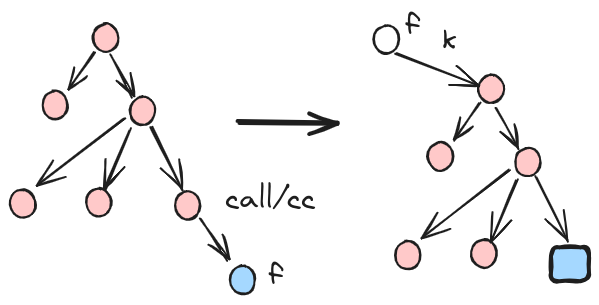
\includegraphics[width=0.6\linewidth]{/home/yukio/Diary/projs/fpcourse/fp-2024/docs/figs/call-cc}
    \caption{\texttt{call/cc} вызывает функцию \texttt{f} с продолжением \texttt{k}.
    Аргумент \texttt{k} (или результат \texttt{f}) подставляется вместо вхождения \texttt{call/cc}.}
    \label{fig:call-cc}
\end{figure}

Например, с помощью \texttt{call/cc} можно реализовать кооперативную многозадачность\footnote{\href{https://en.wikibooks.org/wiki/Haskell/Continuation_passing_style\#Example:_coroutines}{(wiki) Continuation-passing style.
Example: coroutines.}}.
Однако, считается, что \texttt{call/cc} --- не самый удачный примитив\footnote{\url{https://okmij.org/ftp/continuations/against-callcc.html}}.

\subsubsection{Continuation semantics}

Существует стиль формальных семантики, называемый \vocab{continuation semantics}.
Фактически он соответствует написанию определяющих интерпретаторов в CPS\footnote{\url{https://ncatlab.org/nlab/show/continuation-passing+style}}.

Заметьте, что то, что мы строили выше, является shallow embedding некоторого языка, заданного в continuation semantics.
Реализация интерпретатора для deep embedding из~\ref{subsubsec:h-syntax}, например, будет выглядеть следующим образом:
\begin{minted}{haskell}
    eval3' :: Term3 ty -> (forall r . (ty -> r) -> r)
    eval3' term k = case term of
      Val3 x -> k x
      Plus l r -> eval3' l \l' -> eval3' r \r' -> k (l' + r')
      App3 f arg -> eval3' f \f' -> eval3' arg \arg' -> k (f' arg')
      Lam3 f -> k \arg -> eval3' (f (Val3 arg)) id
\end{minted}

Язык с CPS интерпретатором расширить управляющими конструкциями вроде \texttt{call/cc}.
Также можно заметить, что реализация интерпретатора стала хвостово-рекурсивной, а стратегии больше не определяется мета-языком~\cite{reynolds1972definitional}.

% todo call/cc

Проследить семантику операций также можно в следующей нотации, эксплицирующей продолжения:

\begin{align*}
    E[abort(e)] &\rightsquigarrow e\\
    E[call/cc(f)] &\rightsquigarrow E[f(\lambda x\ldotp E[x])]
\end{align*}

\subsubsection{Эффективный CPS}

В нашей реализации CPS производится огромное количество аллокаций замыканий, реифицирующих продолжения.
Однако, если CPS получается автоматической трансляцией, можно делать эффективнее.
Изначально продолжения придумывались для описания семантики прыжков, но можно пойти и в обратную сторону, реализовав продолжения эффективно для современных машин через \texttt{goto}.

Так, состояние функции целиком один раз аллоцируется в куче, а перемещения по телу реализованы как машина состояний --- с помощью меток и прыжков.
Таким образом, например, реализованы безстековые корутины в Kotlin\footnote{\url{https://github.com/Kotlin/KEEP/blob/master/proposals/coroutines.md\#state-machines} \label{note:kotlin-state}}, генераторы в C\#\footnote{\url{https://csharpindepth.com/Articles/IteratorBlockImplementation}}\ldots

Даже в таком виде CPS остаётся тяжеловесной трансформацией, способной замедлить исполнение кода на порядки.
Дело, в частности, в том, что переменные в таком подходе сложно размещать в регистрах (у функций много точек выходов и входов\footref{note:kotlin-state}), приходится постоянно записывать их в RAM --- производить spilling\footnote{\url{https://en.wikipedia.org/wiki/Register_allocation}}.

\subsection{Дефункционализация продолжений}

\footnote{\url{https://ncatlab.org/nlab/show/defunctionalization}}

\cite{reynolds1972definitional}

% todo zipper and nested continuations

% todo huet zipper

% todo zipper context and derivations

% todo abstract machines

% todo

\subsection{Delimited continuations}

Ранее мы рассматривали \vocab{неограниченные (undelimited) продолжения} (или subcontinuations), которые представляют собой весь остаток программы до её конца.
В том числе, мы рассматривали оператор \texttt{call/cc}, который реифицирует неограниченное продолжение в виде функции для непосредственного использования пользователем.
Однако, предоставление пользователю неограниченных продолжений ведёт к множеству проблем и не очень полезно на практике~\footnote{\url{https://okmij.org/ftp/continuations/against-callcc.html}}.

Более того, неограниченные продолжения де-факто --- не совсем функции, так как они не возвращают результата (он уже ``beyond the grave''), следовательно, они также не композируются (как и странно композировать \texttt{abort} с \texttt{exit})\footnote{\url{https://okmij.org/ftp/continuations/undelimited.html}}.
Неограниченные продолжения --- это скорее ко-значения, пока часть программы выполняется, они ожидают её результата~\cite{curien2000duality}.

Вместо этого вводятся парные операторы для работы с \vocab{ограниченными (delimited) продолжениями}\footnote{\url{https://www.cl.cam.ac.uk/teaching/2324/R277/handout-delimited-continuations.pdf}}\footnote{\href{https://youtu.be/TE48LsgVlIU?si=cBdUCzYwYWpwPkkh}{(youtube)  Keynote: Delimited Continuations, Demystified by Alexis King | Lambda Days 2023}.}.
Один позволяет пользователю ограничить продолжение, второй --- захватить всё продолжение до вхождения первого, ограничивающего, оператора.
Таким образом, всё продолжение нарезается на сегменты, некоторый префикс которых может быть реифицирован.

Например, операция кидания и поимки исключения состоит из конструкции \mintinline{kotlin}|try-catch|, ограничивающей продолжение, и \mintinline{kotlin}|throw|, которая позволяет выкинуть частичное продолжения (не захватывая его):
\[
    E_1[catch\{E_2[throw(v)], f\}] \to E_1[f(v)]
\]

Оказывается, ограниченные продолжения первого класса --- крайне могущественная языковая возможность.
Например, через них можно выразить все монадические и алгебраические эффекты.
Подробнее поговорим об этом в следующих разделах~\ref{sec:monads} и~\ref{sec:effect-handlers}.

\subsubsection{Delimited continuations operators}

В литературе встречается огромное количество операторов, для работы с ограниченными продолжениями~\cite[приложение А]{hillerstrom2022foundations}.
Мы рассмотрим классификацию из классической работы~\cite{dyvbig2007monadic}.

Работа вводит следующий набор синтаксических конструкций (рис.~\ref{fig:prompt-syntax}) для работы с ограниченными продолжениями в дополнение к чистому call-by-value лямбда-исчислению.
Исторически в лиспах неограниченные продолжения были ограничены лишь REPL, отсюда название ограничений --- ``prompt''.

\begin{figure}[h]
    \centering
    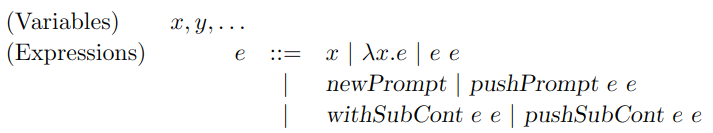
\includegraphics[width=0.75\linewidth]{figs/prompt-syntax}
    \caption{Синтаксис $\lambda$-исчисления с примитивами для работы с продолжениями.}
    \label{fig:prompt-syntax}
\end{figure}

\begin{itemize}
    \item $newPrompt$ --- создаёт свежий идентификатор (метку) ограничения;
    \item $pushPrompt \ap p \ap e$ --- устанавливает ограничение с меткой $p$ и исполняет выражение $e$;
    \item $withSubCont\ap p\ap f$ --- захватывает частичное продолжение до ограничения с меткой $p$ и передаёт в функцию $f$, возвращает результат $f$ (рис.~\ref{fig:push-prompt});
    \item $pushSubCont\ap k \ap v$ --- исполняет композицию текущего продолжения и $k$ на значении $v$.
\end{itemize}

\begin{figure}[h]
    \centering
    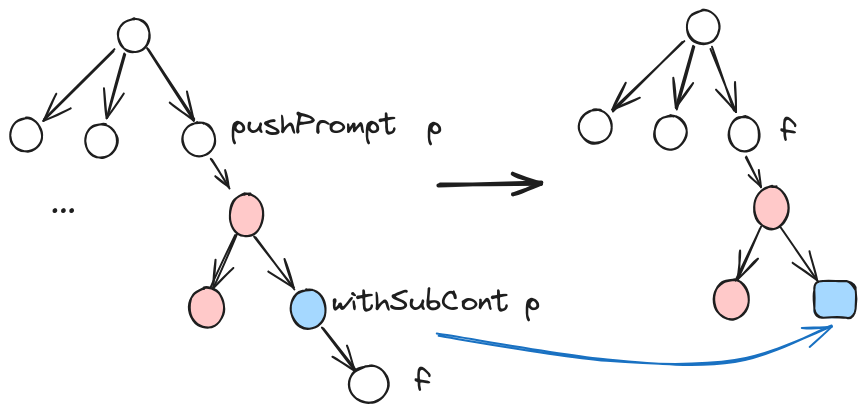
\includegraphics[width=0.7\linewidth]{figs/push-prompt}
    \caption{Пример работы \texttt{withSubCont}.}
    \label{fig:push-prompt}
\end{figure}








% todo in haskell

% todo

\subsubsection{Реализация ограниченных продолжений}

%\subsubsection{State machine}

% todo Cont is for delimited continuations

% todo

%\subsubsection{Continuios stack}

% todo

%\subsubsection{Segmented stack}

% todo

\subsection{Использование продолжений}

% todo trampolining

% todo difference lists

% todo lens

% todo CPS интерпретаторы, переходы

% todo корутины

% todo генераторы

% todo эффекты

% todo transducers, pipelines and internal iteration

% todo CEKT

% todo continuation semantics

% todo continuations and operating systems

% todo single-shot/multi-shot

% todo codensity

% todo problems with continuations: typing and resources

% todo implementing while & break

% todo

% todo control operator, runtime наизнанку

% todo sicp

% todo CPS трансформация интерпретаторов

% todo SPJ compiling without continuations

% todo difference lists

% todo The Essence of Cornpiling with Continuations

% todo calculating correct compilers

% todo reference to best refactoring

%
%    \clearpage


    \section{Эффекты и хендлеры} \label{sec:effect-handlers}
%
%    % todo obsidian What is a purely functional language?
%
%        % todo monad error is a bullshit

    % todo https://homepages.inf.ed.ac.uk/wadler/papers/expression/expression.txt

    % todo https://www.eff-lang.org/handlers-tutorial.pdf

    % todo алгебраические эффекты
    % todo связь с delimited continuations
    % todo стратегии компиляции, связь с codata
    % todo эффекты высших порядков
    % todo full vs shallow embeddings
    % todo abstracting definitional interpreters & github semantics
    % todo fused effects and CPS

    % todo expression problem

    % todo compare open type families & extensible interpreters

    % todo Polymorphic Symmetric Multiple Dispatch with Variance

    % todo \textit{multimethods}

    % todo  custom schedulers

%    Languages with \textit{multimethods}, like Common Lisp’s CLOS, Dylan, and Julia do support adding both new types and operations easily.
%    What they typically sacrifice is either static type checking, or separate compilation.

    % todo ZIO, TS Effect

    % todo inner and outer iteration - The essence of the iterator pattern

    % todo call-by-push value and how it is related to effects

    % todo


    \section{Интерпретаторы зазеркалья} \label{sec:wonder-interpreters}
%
%    %! suppress = MissingLabel

Как мы убедились ранее (см.~\ref{subsec:all-interpreters}), программирование состоит из написания новых и новых интерпретаторов поверх друг друга.
Интерпретаторы задают семантику новых языков (см~\ref{subsubsec:semantics}).
В классическом виде язык задаётся как множество деревьев, а интерпретатор отправляет деревья в объект мета-языка.
Если язык встроенный, то такой подход называют deep embedding (см.~\ref{subsubsec:edsl}).
\[
    \sembr{\bullet} : L \to D
\]

Можно заметить, что в конечном итоге мы используем только элемент домена, в который интерпретатор отображает программу.
Сама программа же представляет собой лишь удобную синтаксическую запись элемента домена и является промежуточным шагом, а не самоцелью.
В то же время доменом в случае встроенных языков, заданных интерпретаторами, являются объекты мета-языка.
Можем ли мы миновать стадию интерпретации собственного синтаксиса и сразу строить объект домена в синтаксисе мета-языка?
Да, такое встраивание называется shallow embedding, о нём эта глава.

\subsection{Формальный путь в зазеркалье}

\subsubsection{Алгебраическое представление типа}

% todo reason isomorphically
% todo connection with cardinalities

% todo isomorphism

\cite[глава 1]{maguire-types}

% todo

\subsection{Tagless final интерпретаторы}

% todo

\subsection{Использование зазеркалья в реальности}

\subsubsection{Expression problem}

% todo







% todo presentation by valera


% todo canonnical sums and products

% todo deforestation of a syntax

% todo visitor pattern














% todo wadler the expression problem

% todo observers

% todo reactive programming https://youtu.be/sTSQlYX5DU0?si=Ybxux16h5Vt1LnC4

% todo pull and push

% todo are custom patterns in haskell connected to this?

% todo вместо того, чтобы доставлять объект к месту деконструирования, доставляем мето деконструирования к месту конструирования

% todo initial and final - isomorphism proof

% todo The Duality of Computation

% todo теоретические основы

% todo church encoding

% todo Tagless-final интерпретаторы

% todo codata, pattern-matching

% todo Extensibility for the Masses: Practical Extensibility with Object Algebras

% todo fusion и дефорестация
% todo haskell inlining
% todo Oleg about fusion and streams
% todo fused effects

% todo codensity

% todo Reading circle about fusion
% todo short cut to deforestation
% todo stream fusion from lists to streams to nothing at all
% todo call-pattern specialization for Haskell programs

% todo композиционность и её восстановление через эксплицирование контекстных зывисимостей.

% todo threaded code

% todo connections to polarity https://ncatlab.org/nlab/show/polarity+in+type+theory

% todo https://okmij.org/ftp/tagless-final/course/Boehm-Berarducci.html

\cite{gibbons2013functional, gibbons2014folding}

% todo

%
%    \clearpage


%    \section{Дополнительные главы монад} \label{sec:monads}
%
%    % todo merriage of effects and monads

% todo ncatlabs

% todo Monads and algebras

% todo оригинальная статья

% todo связь с континуэйшенами

% todo mother of all monads

% todo Stackless Scala with free monads

% todo monadic reflection
% todo monadic reflection & direct style (lib from scala)

% todo free monads, freer monads

% todo монады не композируются, но фримонады - композируются

% todo semantic domains have monad structure

% todo https://github.com/lampepfl/monadic-reflection/blob/main/TUTORIAL.md

% todo C# expression trees
% todo F# что-то про монады и forM

% todo call by push value

% todo monads in pythong with nice syntax

% todo lazyness
% todo direct style

% todo Monads and composable continuations by Phill Wadler

% todo Representing Monads Filinsky
% todo paper delimited continuations in WebAssembly

% todo


    \section{Системы эффектов} \label{sec:effect-systems}
%
%    
% todo merriage of effects and monads

% todo

%
%    \clearpage


    \section{Datatype-generic programming} \label{sec:datatype-generic}
%
%    %! suppress = MissingLabel

Ранее мы говорили о том, что всё, что пишут программисты, --- интерпретаторы.
Оказывается, многие из них можно получать автоматически, выйдя на новый уровень обобщения.
А код, который может не быть написан, --- не должен быть написан.

Как правило, такая ситуация возникает, когда интерпретация полностью определяется описанием (формой) типа.
То есть тем, какие конструкторы данных для него определены, с какими полями, как они называются\ldots
Такими интерпретациями являются, например, сериализация в конеретный формат (e.g. json), структурное равенство и т.д.

Решением является поддержка в языке \vocab{структурного полиморфизма} \vocab{(structural polymorphism)}~\cite[глава 13]{maguire-types} или \vocab{datatype-generic программирование}~\cite{backhousedatatype}, как это иногда называют.

% todo не хотим писать код, который можно не писать

Можно вообразить язык, в котором data-generic программирование является обычным программированием~\cite{chapman2010gentle}.
Для этого берётся язык с зависимыми типами, с выделенной вселенной описаний \mintinline{haskell}|Desc|.
Конкретные типы же получаются применением функции интерпретации \mintinline{haskell}|Desc -> Type|.
Таким образом, параметрический полиморфизм воплощается обобщением по типу, а структурный полиморфизм --- обобщением по его описанию.



% todo generics and Gibbons paper about abstractions

% todo Derivable type classes paper

TODO % todo

\subsection{Специализация}

\[
    \sembr{\sembr{spec}(p, x)}(y) \equiv \sembr{p}(x, y)
\]

% todo специализация в Haskell

% todo staged programming

% todo incremental computations

% todo Zig

% todo Oleg's finally tagless partially evaluated paper

% todo modal types for staged programming

TODO % todo

\subsection{Подходы к datatype-generic в Haskell}

TODO % todo https://ora.ox.ac.uk/objects/uuid:cd041aa0-8d69-4f18-bce2-6d75244b69b9/files/m7fd9779b27fcb70ae734e66bcd3ee79f

\subsubsection{Template Haskel}

% todo Рефлексия и реификация

% todo порядок на коде для поддержания реификации

% todo hygene macro & dynamic scoping

% todo Staging with Class

TODO % todo

\subsubsection{Deriving strategies}

% todo deriving via & Kotlin delegates
% todo newtype derivings & coersions & kotlin delegates

% todo https://ryanglscott.github.io/2018/06/22/quantifiedconstraints-and-the-trouble-with-traversable/

TODO

\subsubsection{GHC.Generics}

TODO % todo

\subsubsection{Sum Of Products}

TODO % todo SOP & variadics

\subsubsection{Uniplate}

% todo SYB

TODO % todo

% todo Kotlinx serialization

% todo datatype-generic для интерпретаторов зазеркалья

%
%    \clearpage


    \section{Персистентность и оптика}
%
%    %! suppress = MissingLabel

Рассмотрим самую вершину башни интерпретаторов.
Там интерпретируется программа, которая сама по себе уже не является интерпретатором, а представляет собой API или UI запрос от внешнего мира.
Эта программа интерпретируется в некоторое преобразование данных $d_{in}\rightsquigarrow d_{out}$, которые в свою очередь уже не являются программой (поскольку им не даётся семантика).
Как выглядят эти преобразования, как их композиционно описывать?

\[
    d_{out} =
    U^{App}\left(
    \left<
    U_{App}^{API/UI},
    \left<
    p_{API/UI},
    d_{in}
    \right>
    \right>
    \right)
\]

Решением является \vocab{функциональная оптика}.
Она позволяет фокусироваться на некоторые свойства объекта и персистентно восстанавливать целый объект с новым значением свойств.
Разные средства фокусировки классифицируют как различные \vocab{оптические девайсы} по интерфейсу использования.
Например, линза может фокусироваться на знак числа, позволяя его просматривать и устанавливать.
Это свойство имеет тип \mintinline{haskell}|Bool|:
\begin{minted}{haskell}
    sign :: Lens' Int Bool
\end{minted}

Существует множество библиотек оптики как для Haskell\footnote{\url{https://hackage.haskell.org/package/optics-0.1/docs/Optics.html}}\footnote{\url{http://lens.github.io/}}\footnote{\url{https://github.com/marcosh/existential-optics/tree/main}}, так и для других языков: Kotlin\footnote{\url{https://arrow-kt.io/}}, Scala\footnote{\url{https://github.com/optics-dev/Monocle}}, Swift\footnote{\url{https://github.com/swiftlang/swift-evolution/blob/main/proposals/0161-key-paths.md}} (языковая поддержка).

\subsection{Персистентные структуры данных}

Структуры данных разделяют на \vocab{изменяемые (mutable)} и \vocab{неизменяемые (immutable)}.
Это классификация лишь по внутренней реализации, используются изменяемые ячейки памяти или нет.

По использованию выделают \vocab{эфемерные} и \vocab{персистентные} структуры данных.
После работы с эфемерной структурой, по той же ссылке может быть доступна другая структура.
\begin{minted}{kotlin}
    let xs = emptyMutableList<Int>()
    xs.add(42)
    print(xs)
\end{minted}

Работа с персистентными структурами порождает каждый раз новые ссылки, в то время как по старым доступна изначальная структура.
\begin{minted}{haskell}
    let xs = []
    let xs' = 42 : xs
    print xs'
\end{minted}

Может показаться, что эфемерные являются изменяемыми, а персистентные --- неизменяемыми.
На самом деле это более-менее ортогональные классификации.
Так, с помощью копирования можно к изменяемой структуре данных предоставить персистентный интерфейс, а неизменяемой --- эфемерный (с помощью монады \mintinline{haskell}|State|).

В речи, когда говорят о персистентных структурах данных, часто имеют в виду структуры данных с персистентным интерфейсом, специально оптимизированные для него (не требуют полного копирования на каждую операцию).
Способы построения таких структур и работы с ними на удивление довольно оптимальны и разнообразны~\cite{okasaki1999purely}.

Например, можно реализовать эффективный персистентный массив с логарифмической сложностью всех операций.
В Haskell такой структурой данных является \mintinline{haskell}|Seq|\footnote{\url{https://hackage.haskell.org/package/containers-0.7/docs/Data-Sequence.html}}\footnote{\url{http://www.staff.city.ac.uk/~ross/papers/FingerTree.html}}.
Если в вершинах хранить небольшие массивы, которые современные аритектуры процессоров могут эффективно копировать, можно существенно уменьшить высоту дерева и алгоритмическую сложность операций (e.g. \mintinline{scala}|scala.immutable.Vector|).

\begin{task}
    Реализуйте не Haskell персистентное декартово дерево по неявному ключу.
    Какие особенности Haskell усложняют использование этой структуры?
\end{task}

Когда использовать эфемерные, а когда персистентные структуры данных?
Если сравнивать, то можно обнаружить, что эфемерные можно реализовывать эффективнее во многих случаях, так как память изменяемая и кеши процессоров лучше работают с локальными данными (в то время как персистентные структуры обречены быть деревьями, чтобы реаллоцировать не структуру целиком, а только путь до корня).

Персистентные структуры же позволяют писать более модульный и безопасный с точки зрения многопоточности код, который может не учитывать возможность изменения структуры по ссылке.
В то время как работа с эфемерной структурой не является чистым кодом, а включает в себя порождение побочных эффектов.
Также объединение персистентными результатов разных вызовов может быть дешевле, как, например, конкатенация персистентных массивов дешевле конкатенации эфемерных (логарифмическая сложность против линейной).

Таким образом, в рамках ограниченного, легко обозреваемого скоупа лучше использовать эфемерные структуры ввиду их эффективности (например, чтобы изначально заполнить коллекцию элементами).
Однако, через границы абстракции лучше пропускать только персистентные структуры (или же положиться на систему эффектов, см.~\ref{sec:effect-systems}).
То есть каждая структура данных должна поддерживать две фазы своей жизни.
Например, так сделано в Scala, где у многих персистентных коллекций есть \mintinline{scala}|Builder| версия.

\subsection{Простейшая оптика}

Линзы являются простейшим примером оптического девайса.
Они позволяют гарантированно обозревать одно свойство и устанавливать его.

Изначально линзы были предложены как решение проблемы view-update в базах данных~\cite{bohannon2006relational, foster2008quotient}.
А именно --- как нужно изменить реальную базу при изменении view.
Или как восстанавливать целое после извлечения и изменения части.
Линзы тут являются средством двустороннего программирования --- позволяют одновременно описывать как view, так и способ обновления.

Параллельно\footnote{\url{https://github.com/ekmett/lens/wiki/History-of-Lenses}}, линзы упоминаются в серии блог-постов, описывающих попытку удобнее работать с изменяемым состоянием при написании игр\footnote{\href{https://web.archive.org/web/20140402193032/https://lukepalmer.wordpress.com/2007/07/26/making-haskell-nicer-for-game-programming/}{(post) Making Haskell nicer for game programming}}\footnote{\href{https://web.archive.org/web/20120303223802/https://lukepalmer.wordpress.com/2007/08/05/haskell-state-accessors-second-attempt-composability/}{(post) Haskell State Accessors (second attempt: Composability)}} (линзы в играх продолжают радовать\footnote{\url{http://www.timphilipwilliams.com/posts/2019-07-25-minecraft.html}}).

\subsubsection{Линзы --- costate coalgebra comonad}

% todo картинки

Простейшую линзу образуют пара функций --- просмотр и установка свойства:
\begin{minted}{haskell}
    data SimpleLens' s a = SimpleLens'
      { view' :: s -> a
      , set' :: s -> a -> s
      }
\end{minted}

На эти функции накладываются естественные законы:
\begin{minted}{haskell}
    view l (set l s x) ?$\equiv$? x
    set l s (view l s) ?$\equiv$? s
    set l (view l s x) y ?$\equiv$? set l s y
\end{minted}

Линзы можно композировать и обращаться к вложенным полям произведений.
Так, они могут быть морфизмами в категории типов.
При таком определении, правда, композиция работает в обратном, от желаемого, порядке.
\begin{minted}{haskell}
    instance Category SimpleLens' where
      id :: SimpleLens' s s
      id = SimpleLens' { view' = id, set' = flip const }

      (.) :: SimpleLens' a b -> SimpleLens' s a -> SimpleLens' s b
      l1 . l2 = SimpleLens'
        { view' = view' l1 . view' l2
        , set' = \s x -> set' l2 s (set' l1 (view' l2 s) x)
        }
\end{minted}

Например, можно легко изменить возраст пользователя:
\begin{minted}{haskell}
    newtype Age = Age { _getAge :: Int }
    data User = User { _userName :: String, _userAge :: Age }

    userAge :: SimpleLens' User Age
    userAge = SimpleLens' { view' = _userAge, set' = \s x -> s { _userAge = x } }

    getAge :: SimpleLens' Age Int
    getAge = SimpleLens' { view' = _getAge, set' = \s x -> s { _getAge = x } }

    ghci> set (getAge . userAge) user 1
\end{minted}

Можно обобщить линзы до полиморфных линз, которые позволяют пересоздавать структуру с новыми типовыми параметрами:
\begin{minted}{haskell}
    data SimpleLens s t a b = SimpleLens
      { view :: s -> a
      , set :: s -> b -> t
      }

    _1 :: SimpleLens (a, c) (b, c) a b
    _1 = SimpleLens { view = \(x, _) -> x, set = \(x, c) y -> (y, c) }
\end{minted}

Можно заметить, что линза в таком представлении является комонадой коалгеброй коstate\footnote{\href{https://youtu.be/9_iYlp8smc8?si=NLka0vnnhYDdTfgm}{(youtube) Category Theory II 9.1: Lenses.}}.
Действительно, пару функций можно заменить на функцию, возвращающую пару:
\begin{minted}{haskell}
    data Store a s = Store (a, a -> s)
    data DataLens s a = DataLens (s -> Store a s)
\end{minted}

Если определить инстанс комонады для \mintinline{haskell}|Store a s| и выписать законы совместимости с коалгеброй, мы получим в точности законы линз.

\subsubsection{Призмы}

Призмы позволяют получить свойство, которое может отсутствовать, и устанавливать его при наличии.
Так, конкретное поле типа-суммы может не удаться извлечь, при передаче не ожидаемого конструктора.

Простые призмы можно определить аналогично линзам, с учётом возможного отсутствия свойства:

\begin{minted}{haskell}
    data SimplePrism' s a = SimplePrism'
      { preview' :: s -> Maybe a
      , review' :: a -> s
      }
\end{minted}

Полиморфная призма должна предоставить структуру с обновлённым типом в случае неуспеха просмотра:
\begin{minted}{haskell}
    data SimplePrism s t a b = SimplePrism
      { preview :: s -> Either t a
      , review :: b -> t
      }
\end{minted}

Можно определить призму для работы с содержимым конструктора \mintinline{haskell}|Left|:
\begin{minted}{haskell}
    _Left :: SimplePrism (Either a c) (Either b c) a b
    _Left = SimplePrism
      { preview = \case Left a -> Right a; Right c -> Left (Right c)
      , review = Left
      }
\end{minted}

Композиция призм определяется естественным образом.

\subsubsection{Композиция линз и призм}

Заведём класс типов, с помощью которого научимся композировать различные комбинации линз и призм.
Результирующий девайс однозначно определяется операндами композиции.

\begin{minted}{haskell}
    class Composable o1 o2 o3 | o1 o2 -> o3 where
      compose :: o1 s t a b -> o2 a b c d -> o3 s t c d
\end{minted}

Теперь можем естественным образом определить композицию для различных девайсов.
Можно заметить, что этот подход требует квадратичное количество инстансов от количества оптических девайсов.

\begin{minted}{haskell}
    instance Composable SimpleLens SimpleLens SimpleLens where
      compose :: SimpleLens s t a b -> SimpleLens a b c d -> SimpleLens s t c d
      compose l2 l1 = SimpleLens
        { view = view l1 . view l2
        , set = \s x -> set l2 s (set l1 (view l2 s) x)
        }
\end{minted}

Композиция линз и призм образует другой девайс --- аффинные траверсы, которые являются чем-то средним.
Наличие призмы в композиции не позволяет гарантированно просматривать свойство, а линзы --- создавать новое значение без изначального.
\begin{minted}{haskell}
    data AffineTraversal s t a b = AffineTraversal
      { apreview :: s -> Either t a
      , aset :: s -> b -> t
      }

    instance Composable SimplePrism SimpleLens SimplePrism where
      compose :: SimplePrism s t a b -> SimpleLens a b c d -> SimplePrism s t c d
      compose p l = SimplePrism
        { preview = fmap (view l) . preview p
        , pset = \s d -> case preview p s of
            Left t -> t
            Right a -> pset p s (set l a d)
        }
\end{minted}

\subsection{Разнообразие оптических девайсов, \texttt{optics}} \label{subsec:optics}

Различных оптических девайсов можно придумать довольно много.
Библиотека \texttt{optics} предоставляет абстрактный интерфейс для самых популярных из них (рис.~\ref{fig:optics-hierarchy}).
Она имеет прекрасную документацию с подробным описанием девайсов\footnote{\url{https://hackage.haskell.org/package/optics-0.4.2.1/docs/Optics.html}}.

\begin{figure}
    \centering
    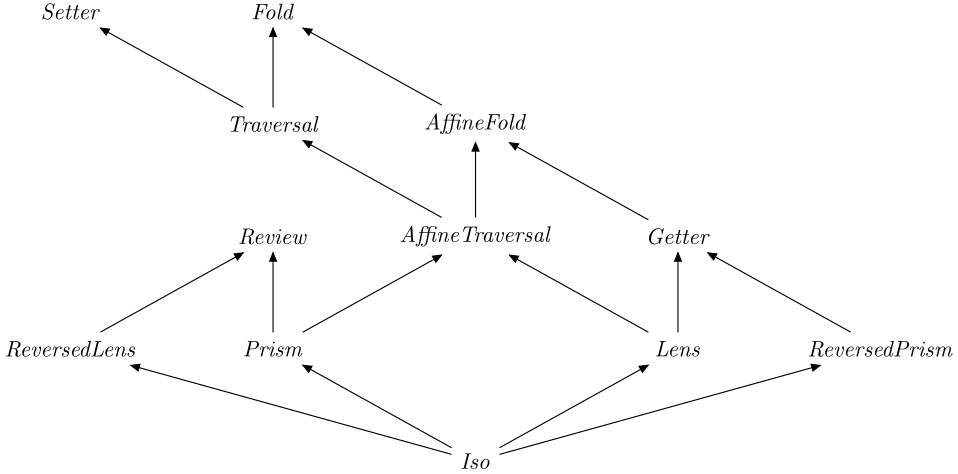
\includegraphics[width=\textwidth]{/home/yukio/Diary/projs/fpcourse/fp-2024/docs/figs/optics-hierarchy}
    \caption{Иерархия оптических девайсов \texttt{optics}.}
    \label{fig:optics-hierarchy}
\end{figure}

Примеры:
\begin{minted}{haskell}
    data Pet = Cat String | Dog Int deriving Show
    newtype UserName = UserName { _getUserName :: String } deriving Show
    data User = User { _userName :: UserName, _userCats :: [Pet] } deriving Show

    exampleUser :: User
    exampleUser = User (UserName "Bob") [Cat "Kitty", Dog 42, Dog 4]

    exampleName :: User -> User
    exampleName = over (userName % getUserName) (++ "!")

    exampleIx :: User -> User
    exampleIx = set (userName % getUserName % ix 2) 'k'

    exampleFold :: User -> Int
    exampleFold = getSum $ foldMapOf (userName % getUserName % folded) (const 1)

    examplePrint :: User -> IO User
    examplePrint = traverseOf (userCats % traversed % _Dog) (\x -> x <$ print x)
\end{minted}

\subsection{Другие представления оптики}

Ранее мы рассмотрели тривиальную оптику, составленную непосредственно из кортежа элиминирующих функций (пары разбора-пересборки значений).
Однако, у такого подхода есть существенные недостатки.
Во-первых, нужно определять много операций композиции для различных видов оптики.
То есть композиция девайсов --- что-то гораздо более сложное, чем композиция функций.
Во-вторых, это представление не очень эффективно, так как сложно представить, что компилятор будет инлайнить вызовы функций из структур данных.

Было приложено много усилий и теорката\footnote{\url{https://bartoszmilewski.com/category/lens/}}, чтобы получить другие представления оптики.
Некоторые из них являются просто одной функцией, кодирующей все нужные преобразования, а композиция определена как композиция таких функций.

\subsubsection{Semantic editor combinators}

TODO semantic editor combinators\footnote{\url{http://conal.net/blog/posts/semantic-editor-combinators}} % todo

\subsubsection{Линзы ван Лаарховена}

TODO van Laarhoven lens\footnote{\url{https://www.twanvl.nl/blog/haskell/cps-functional-references}}\footnote{\href{http://r6.ca/blog/20120623T104901Z.html}{(post) Polymorphic Update with van Laarhoven Lenses}} % todo

TODO lens\footnote{\url{http://lens.github.io/}} % todo

% todo uniplate

\subsubsection{Profunctor optics}

TODO % todo немножко profunctor optics

% todo ссылки на Бартоша

\subsubsection{Existential (coend) optics}

TODO\footnote{\url{https://github.com/marcosh/existential-optics/tree/main}}\footnote{\url{https://www.tweag.io/blog/2022-05-05-existential-optics/}}\footnote{\url{https://www.twanvl.nl/blog/haskell/isomorphism-lenses}}\footnote{\url{https://www.brunogavranovic.com/posts/2022-01-05-lenses-to-the-left-of-me.html}} % todo


\subsection{Генерация оптики}

Чтобы использовать оптику для работы со своими структурами данных, нужно так или иначе получить для них реализацию девайсов.

Некоторую специфичную оптику можно написать руками.
Например, позволяющую работать с нетривиальным свойством значения (знак числа, высота дерева\ldots).
Библиотеки предоставляют специальные билдеры, упрощающие конструирование\footnote{\url{https://hackage.haskell.org/package/optics-core-0.1/docs/Optics-Lens.html\#v:lens}}.

Некоторая оптика получается автоматически из инстансов стандартных классов типов.
Например, свёртки и траверсы\footnote{\url{https://hackage.haskell.org/package/optics-core-0.1/docs/Optics-Traversal.html\#g:6}}.
Дальше уже встаёт вопрос о генерации инстансов классов типов (см.~\ref{sec:datatype-generic}).

Поскольку линзы являются просто обобщением полей, а призмы --- конструкторов, их можно генерировать автоматически с помощью макросов по структуре данных\footnote{\url{https://hackage.haskell.org/package/optics-th-0.1/docs/Optics-TH.html}}.
Для этого используются конвенции, поля называются с подчёркиванием, а макрос сгенерирует линзы без подчёркивания.
С призмами наоборот.
Так, генерация для примера выше (\ref{subsec:optics}) будет выглядеть следующим образом:
\begin{minted}{haskell}
    makeLenses ''User
    makeLenses ''UserName
    makePrisms ''Pet
\end{minted}

TODO библиотека  % todo

TODO data-generic optics\footnote{\url{https://hackage.haskell.org/package/optics-core-0.4.1.1/docs/Optics-Label.html}}\footnote{\url{https://ghc.gitlab.haskell.org/ghc/doc/users_guide/exts/overloaded_record_update.html}}\footnote{\url{https://ghc.gitlab.haskell.org/ghc/doc/users_guide/exts/overloaded_labels.html}} % todo

TODO % todo


% todo библиотеки с оптикой для других языков

% todo transducers

% todo слайды Беляева

% todo zippers

% todo сравнение с datatype generic programming

% todo оптика как альтернатива стримам?

% todo first-class patterns should also be able to re-build the values that they match, Pattern Synonyms paper

% todo data processing

% todo https://blog.poisson.chat/
% todo lens and serialization

%
%    \clearpage


    % todo субструктурность, ресурсы....


%%    \section{Компилятор GHC и runtime}
%
%    % todo Working with Source Plugins paper

% todo \href{https://gitlab.haskell.org/ghc/ghc/-/wikis/commentary/compiler/generated-code}{\color{blue} I know kung fu: learning STG by example}

% todo


    % todo куда-нибудь запихнуть algebra driven design, quick check и доклад про проперти-тесты
    % todo Perhaps Not The Answer You Were Expecting But You Asked For It
    % todo link to SICP

    % todo зависимые типы в Haskell

    % todo рассовать упражнений по конспекту

    % todo Wadler's "Introduction to functional programming"

%    \begin{center}
%        \vspace{2em}
%        \textit{\LARGE To be continued...}
%        \vspace{2em}
%    \end{center}


%    \newpage
    \bibliography{bib}

\end{document}
